% chapter: 漸化式の解説

\chapter{漸化式の解説}\label{章：漸化式の解説}
\begin{bookcolumns}
% section: 漸化式の分類

\section{漸化式の分類}\label{節：漸化式の分類}
  \BookFigClassification

  ここまでに使った方法を、一枚の地図として見直す。
  まず\bookterm{recurrence}{漸化式}は解ける\bookterm{recurrence}{漸化式}と解けない\bookterm{recurrence}{漸化式}に分類される.
  そして解ける\bookterm{recurrence}{漸化式}は「決まった手順で解ける\bookterm{recurrence}{漸化式}」と「特定の性質から解ける\bookterm{recurrence}{漸化式}」に分類される.
  「決まった手順で解ける\bookterm{recurrence}{漸化式}」はさらに分類され,各分類ごとに様々な解法がある.
  ここで言う「解ける」というのは,本書内での定義であり,一般的なものではない.
  ここで解けないとして扱われるような\bookterm{recurrence}{漸化式}は\bookterm{general}{一般項}を表す手段が存在しないわけではない.
  あくまで本書で扱う手法の内では表現できないという意味である.
  「解ける」の定義について述べておく.
  定義は,高校数学程度の範囲内で既知の関数に帰着するか,\,$n$に依存しない有限個の\bookterm{elementary}{初等関数}の演算によって\bookterm{general}{一般項}を表せるような解法が存在するものを意味している.
  このうち「決まった手順で解ける\bookterm{recurrence}{漸化式}」は基本4パターン・応用7パターン・発展パターンの各節で,「特定の性質から解ける\bookterm{recurrence}{漸化式}」は特殊性質の節で扱う.

  基本4パターンでは、差と倍率から項を求めた。
  応用パターンでは、追う量を変えることで、その基本形を取り出した。
  発展パターンと特殊性質型では、追う対象と調べる性質がさらに広がった。

  この分類は,解法を探すための案内である.一つの式に複数の解法が使えることもある.
  本書の方法で\bookterm{closed}{閉じた形}が見つからなくても,\bookterm{sequence}{数列}が定義されないわけではなく,\bookterm{limit}{極限}や整数の性質を調べる価値も失われない.
  例えば\bookproblemref{practice-entrance}{6}{発展問6}では,\bookterm{general}{一般項}を求めずに減り方を調べる.

% section: 漸化式を解く前に

\section{漸化式を解く前に}\label{節：漸化式を解く前に}
  \BookFigApproach

  本章で繰り返し使う問いは,「元の項より,次への変化が簡単になる量はないか」である.
  例えば$a_{n+1}=2a_n+3$では,定数$3$があるため等比型の式をそのまま使えない.
  両辺に$3$を加えると
  \[
    a_{n+1}+3=2(a_n+3)
  \]
  となり,\,$b_n=a_n+3$という同じ形の量が2倍されていると分かる.
  なぜ$3$を選ぶかは\sectionref*{節：特性方程式型}で導く.
  ここでは,変形の目標を具体的に持つことを確認しよう.
  \begin{itemize}
    \item $b_{n+1}-b_n=f(n)$なら,変化を足し戻す（階差型）.
    \item $b_{n+1}=f(n)b_n$なら,倍率を掛け合わせる（階比型）.
    \item $b_{n+1}=b_n$なら,その量は初項から変わらない.
    \item 既知の公式と同じ形なら,その公式の入力に当たる量を追う.
  \end{itemize}
  本書で「きれいな形」と呼ぶのは,こうした更新の仕組みを追いやすい形である.
  和や積の表示が得られた後,それをどこまで計算できるかは別に確認する.

  説明を読むときは,\textbf{観察と発想}と\textbf{式変形}を分けて追ってほしい.
  前者では,どの項を消すか,どの倍率をそろえるかを選ぶ.
  後者では,選んだ量を実際に代入し,初項から一般項を求め,元の量へ戻す.
  逆数・対数・割り算を使う前には,その操作が定義できるかも確かめる.
  候補を探す計算の途中で条件が必要だと分かった場合は,そこで条件を確認してから続ける.

  最初の数項を計算する実験も,変形の候補を見つける助けになる.
  数項の一致は予想の根拠であり,すべての項についての証明にはならない.
  予想した式が初期条件と元の更新式を満たせば,順に次の項が一意に決まる漸化式では,数学的帰納法で一致を示せる.
  \sectionref*{節：数学的帰納法}を参照してほしい.
  帰納法は,変形から得た式を確かめるときにも,実験から得た予想を証明するときにも使える.

  一般項を簡単な式で表すことに加えて,正値・極限・整数性などを調べる目標もある.
  \chapterref{章：実際の解き方}では方法の選択を練習し,発展演習と付録では目標の広がりを見る.

% section: 基本4パターン

\section{基本4パターン}\label{節：基本4パターン}
  \BookFigBasicFour

  差が分かれば、変化を足し戻せる。
  倍率が分かれば、その倍率を掛け合わせられる。
  ここでは、差と倍率が一定の場合から、添字によって変わる場合へ進む。
  後の解法では、元の式を変形し、この四つの仕組みを取り出していく。
  特に等比型は、多くの変形の行き先になる。

% subsection: 等差型 \, $a_{n+1}=a_n+d$

  \subsection{\texorpdfstring{等差型 \, $a_{n+1}=a_n+d$}{等差型}}\label{節：等差型}
  \begin{bookpoint}
    \textbf{差を追う}\par
    一回ごとに足す量が一定なら,初項に増分を足し戻す.項の番号と更新の回数の違いを確かめよう.
  \end{bookpoint}
    まずはもっともシンプルな\bookterm{recurrence}{漸化式}であろう,等差型について説明していく.
    この\bookterm{recurrence}{漸化式}は$a_1$に対して$d$がどんどんと足されていく\bookterm{recurrence}{漸化式}である.
    \bookterm{general}{一般項}は簡単な代入計算によって容易に示せる.
    実際にやってみると
    \begin{align*}
      &a_{n+1}=a_n+d\\
      &a_{n+1}=(a_{n-1}+d)+d\\
      &a_{n+1}=\{(a_{n-2}+d)+d\}+d\\
      &\qquad \vdots\\
      &a_{n+1}=a_1+d+d+\cdots+d\\
      &a_{n+1}=a_1+nd\\
      &\therefore \quad a_n=a_1+(n-1)d
    \end{align*}
    となり\bookterm{general}{一般項}が示される.
    1つ前の項をどんどん代入していくのだ.
    数式の3行目から5行目周辺の式変形が少し心配かもしれないが,\,$d$の個数と$a$の添字部分の和は常に$n+1$となることから考えれば分かるだろう.
    実際,\,$a_{n+1}$に至るまでに何度$d$が足されたかを考えているわけだから,心配であれば実際に適当な$n$で何度か実験してみるのもいい手だろう.

    実際に例題を与えよう.

    \noindent \bookblocklink{example-arithmetic-1}{problem}{answer}{【例題】}\par\nobreak
    \begin{enumerate}[label=(\arabic*),parsep=3pt,format=\bookitemlink{example-arithmetic-1}{problem}{answer}]
      \item $\displaystyle a_1=1,\, a_{n+1}=a_n+1$
      \item $\displaystyle a_1=\frac{1}{2},\, a_{n+1}=a_n+\frac{1}{4}$
      \item $\displaystyle a_1=-\sqrt{3},\, a_{n+1}=a_n-\sqrt{2}$
    \end{enumerate}

    \noindent\bookblocklink{example-arithmetic-1}{hint}{problem}{【方針】}\par\nobreak
    \begin{enumerate}[label=(\arabic*),parsep=3pt,format=\bookitemlink{example-arithmetic-1}{hint}{problem}]
      \item 等差型の\bookterm{general}{一般項}
            $\displaystyle a_n=a_1+(n-1)d$
            を用います.
      \item 公差は$\displaystyle d=\frac14$です.
            等差型の\bookterm{general}{一般項}に代入します.
      \item 公差は$\displaystyle d=-\sqrt2$です.
            負の公差の場合も同じ公式を使います.
    \end{enumerate}

    \noindent\bookblocklink{example-arithmetic-1}{answer}{problem}{【解答】}\par\nobreak
    \begin{enumerate}[label=(\arabic*),parsep=3pt,format=\bookitemlink{example-arithmetic-1}{answer}{problem}]
      \item $\displaystyle a_n=1+(n-1)=n$
      \item $\displaystyle a_n=\frac12+\frac{n-1}{4}
            =\frac{n+1}{4}$
      \item $\displaystyle a_n=-\sqrt3-(n-1)\sqrt2$
    \end{enumerate}

    \noindent\bookblocklink{example-arithmetic-1}{solution}{problem}{【解法】}\par\nobreak
    解法略.

% subsection: 等比型 \, $a_{n+1}=ra_n$

  \subsection{\texorpdfstring{等比型 \, $a_{n+1}=ra_n$}{等比型}}\label{節：等比型}
  \begin{bookpoint}
    \textbf{倍率を追う}\par
    一回ごとの倍率が一定なら,更新の回数だけ掛ける.公比が零の場合も,比で割らず更新の式から読む.
  \end{bookpoint}
    次に説明するのは等比型である.
    一般的な解法も先ほどと同じで,\,$a_{n+1}$から順に$a_1$に向けて書き下して行くことで求めることができる.
    \begin{align*}
      &a_{n+1}=ra_n\\
      &a_{n+1}=r(ra_{n-1})\\
      &a_{n+1}=r\{r(ra_{n-2})\}\\
      &\qquad \vdots\\
      &a_{n+1}=r\cdot r \cdot \cdots \cdot ra_1\\
      &a_{n+1}=a_1r^n\\
      &\therefore \quad a_n=a_1r^{n-1}
    \end{align*}

    \noindent \bookblocklink{example-geometric-1}{problem}{answer}{【例題】}\par\nobreak
    \begin{enumerate}[label=(\arabic*),parsep=3pt,format=\bookitemlink{example-geometric-1}{problem}{answer}]
      \item $\displaystyle a_1=1,\, a_{n+1}=2a_n$
      \item $\displaystyle a_1=1,\, a_{n+1}=-a_n$
      \item $\displaystyle a_1=2,\, a_{n+1}=\frac{1}{2}a_n$
    \end{enumerate}

    \noindent\bookblocklink{example-geometric-1}{hint}{problem}{【方針】}\par\nobreak
    \begin{enumerate}[label=(\arabic*),parsep=3pt,format=\bookitemlink{example-geometric-1}{hint}{problem}]
      \item 等比型の\bookterm{general}{一般項}
            $\displaystyle a_n=a_1r^{n-1}$
            を用います.
      \item 公比は$r=-1$です.
            符号が交互に変化することに注意します.
      \item 初項と公比を\bookterm{general}{一般項}に代入します.
    \end{enumerate}

    \noindent\bookblocklink{example-geometric-1}{answer}{problem}{【解答】}\par\nobreak
    \begin{enumerate}[label=(\arabic*),parsep=3pt,format=\bookitemlink{example-geometric-1}{answer}{problem}]
      \item $\displaystyle a_n=2^{n-1}$
      \item $\displaystyle a_n=(-1)^{n-1}$
      \item $\displaystyle a_n=2\left(\frac12\right)^{n-1}$
    \end{enumerate}

    \noindent\bookblocklink{example-geometric-1}{solution}{problem}{【解法】}\par\nobreak
    解法略.

% subsection: 階差型 \, $a_{n+1}=a_n+f(n)$

  \subsection{\texorpdfstring{階差型 \, $a_{n+1}=a_n+f(n)$}{階差型}}\label{節：階差型}
  \begin{bookpoint}
    \textbf{変化を足す}\par
    差が添字ごとに変わっても,初項からの変化を足せば元の項に戻る.和の範囲は実際の更新の回数に合わせる.
  \end{bookpoint}
    足す量が一定でなくても、初項からの変化を足し戻せる。
    一歩目では$f(1)$、二歩目では$f(2)$を足す。
    直前の項を代入すると、その変化が順に並ぶ。
    \begin{align*}
      &a_{n+1}=a_n+f(n)\\
      &a_{n+1}=\{a_{n-1}+f(n-1)\}+f(n)\\
      &a_{n+1}=\left[\{a_{n-2}+f(n-2)\}+f(n-1)\right]+f(n)\\
      &\qquad \vdots\\
      &a_{n+1}=a_1+f(1)+f(2)+\cdots+f(n)\\
      &a_{n+1}=a_1+\sum_{k=1}^{n} f(k)\\
      &\therefore \quad a_n=a_1+\sum_{k=1}^{n-1} f(k)
    \end{align*}
    変化を足すところまでで、元の\bookterm{sequence}{数列}は和の形に表せた。
    残るのは、その和の計算である。
    $f(n)$の形に合わせて、\bookterm{arithmetic}{等差数列}の和、\bookterm{geometric}{等比数列}の和、\bookterm{partial}{部分分数分解}を使う。

    \noindent \bookblocklink{example-difference-1}{problem}{answer}{【例題】}\par\nobreak
    \begin{enumerate}[label=(\arabic*),parsep=3pt,format=\bookitemlink{example-difference-1}{problem}{answer}]
      \item $\displaystyle a_1=1,\, a_{n+1}=a_n+n$
      \item $\displaystyle a_1=1,\, a_{n+1}=a_n+2^n$
      \item $\displaystyle a_1=0,\, a_{n+1}=a_n+\frac{1}{n(n+1)}$
      \item $\displaystyle a_1=1,\, a_{n+1}=a_n+(n+1)^2$
    \end{enumerate}

    \noindent\bookblocklink{example-difference-1}{hint}{problem}{【方針】}\par\nobreak
    \begin{enumerate}[label=(\arabic*),parsep=3pt,format=\bookitemlink{example-difference-1}{hint}{problem}]
      \item 足す量は$n$です。初項からの変化を、一次式の和にまとめます。
      \item もちろん,\,$f(n)$となる関数には指数関数も含まれます.何にせよやることは\,(1)と同じです.
      \item \bookterm{sigma}{シグマ}は\bookterm{partial}{部分分数分解}で処理しましょう.
      \item 足す量は$(n+1)^2$です。初項を含めて、平方の和としてまとめます。
    \end{enumerate}

    \noindent\bookblocklink{example-difference-1}{answer}{problem}{【解答】}\par\nobreak
    \begin{enumerate}[label=(\arabic*),parsep=3pt,format=\bookitemlink{example-difference-1}{answer}{problem}]
      \item $\displaystyle a_n=1+\frac{n(n-1)}{2}$
      \item $\displaystyle a_n=2^n-1$
      \item $\displaystyle a_n=1-\frac{1}{n}$
      \item $\displaystyle a_n=\frac{1}{6}n(n+1)(2n+1)$
    \end{enumerate}

    \noindent\bookblocklink{example-difference-1}{solution}{problem}{【解法】}\par\nobreak
    \begin{enumerate}[label=(\arabic*),parsep=3pt,format=\bookitemlink{example-difference-1}{solution}{problem}]
      \item $\displaystyle a_1=1,\,a_{n+1}=a_n+n$\\
            \bookterm{difference}{階差}型の\bookterm{general}{一般項}
            \[
              a_n=a_1+\sum_{k=1}^{n-1}f(k)
            \]
            を用いると,
            \begin{align*}
              a_n
                &=1+\sum_{k=1}^{n-1}k\\
                &=1+\frac{n(n-1)}{2}
            \end{align*}

      \item $\displaystyle a_1=1,\,a_{n+1}=a_n+2^n$\\
            同様に,
            \begin{align*}
              a_n
                &=1+\sum_{k=1}^{n-1}2^k\\
                &=1+(2+2^2+\cdots+2^{n-1})\\
                &=1+(2^n-2)\\
                &=2^n-1
            \end{align*}

      \item $\displaystyle a_1=0,\,a_{n+1}=a_n+\frac{1}{n(n+1)}$\\
            \bookterm{partial}{部分分数分解}を用いると,
            \[
              \frac{1}{k(k+1)}
              =\frac{1}{k}-\frac{1}{k+1}
            \]
            であるから,
            \begin{align*}
              a_n
                &=\sum_{k=1}^{n-1}\frac{1}{k(k+1)}\\
                &=\sum_{k=1}^{n-1}
                  \left(\frac{1}{k}-\frac{1}{k+1}\right)\\
                &=\left(1-\frac12\right)
                  +\left(\frac12-\frac13\right)\\
                &\quad +\cdots+\left(\frac{1}{n-1}-\frac1n\right)\\
                &=1-\frac1n
            \end{align*}

      \item $\displaystyle a_1=1,\,a_{n+1}=a_n+(n+1)^2$\\
            \bookterm{difference}{階差}型の\bookterm{general}{一般項}を用いると,
            \begin{align*}
              a_n
                &=1+\sum_{k=1}^{n-1}(k+1)^2\\
                &=1+\sum_{j=2}^{n}j^2\\
                &=\sum_{j=1}^{n}j^2\\
                &=\frac{1}{6}n(n+1)(2n+1)
            \end{align*}
    \end{enumerate}

% subsection: 階比型 \, $a_{n+1}=f(n)a_n$

  \subsection{\texorpdfstring{階比型 \, $a_{n+1}=f(n)a_n$}{階比型}}\label{節：階比型}
  \begin{bookpoint}
    \textbf{倍率を掛ける}\par
    添字ごとの倍率を掛け合わせる方法と,その倍率に合う因子で割る方法を比べよう.零で割らない条件は共通である.
  \end{bookpoint}
    \bookterm{difference}{階差}型では変化を足した.ここでは,各段階の倍率を掛け合わせる.
    難しい点は,積を計算することと,倍率をそろえる因子を見つけることに分かれる.
    まず積の表示を学び,その後に\bookterm{normalize}{正規化}の因子を選ぶ理由を見る.

    具体的な説明の前に1つだけ記号を新たに導入しておく.
    適当な数が並べられた\bookterm{sequence}{数列}$x_n$が存在した時,
    \[
      \prod_{i=1}^n x_i
      =x_1\times x_2\times\cdots\times x_n
    \]
    となるような記号$\prod$（ラージパイ）を定義する.
    これを\bookterm{product}{総積}記号といい,積を表す.
    また,一般に以下が成り立つ.
    \begin{align*}
      &\prod_{i=1}^{n}i=n!\\
      &\prod_{i=1}^{n}k=k^n\\
      &\prod_{i=1}^{n}a_ib_i=\displaystyle\prod_{i=1}^na_i\displaystyle\prod_{i=1}^nb_i\\
      &\prod_{i=1}^{n}a_i=\displaystyle\prod_{i=1+k}^{n+k}a_{i-k}\\
      &\prod_{i=1}^{n}(i+k)=\dfrac{(n+k)!}{k!}
    \end{align*}
    ここでの$a_i$や$b_i$は\bookterm{recurrence}{漸化式}等によって定義されるような,法則性を持った\bookterm{sequence}{数列}である必要はなく,
    「1から順に番号が振られた,数の並び」ぐらいのイメージで問題ない.
    では再び, \,$a_n$の\bookterm{general}{一般項}を求めていく.
    \begin{align*}
      &a_{n+1}=f(n)a_n\\
      &a_{n+1}=f(n)\{f(n-1)a_{n-1}\}\\
      &a_{n+1}=f(n)\left[f(n-1)\{f(n-2)a_{n-2}\}\right]\\
      &\qquad \vdots\\
      &a_{n+1}=f(1)f(2) \cdots f(n)a_1\\
      &a_{n+1}=a_1 \prod_{k=1}^n f(k)\\
      &\therefore \quad a_n=a_1 \prod_{k=1}^{n-1} f(k)
    \end{align*}
    この積による表示は$f(k)=0$となる場合も成り立つ(空積は$1$とする).
    \noindent \bookblocklink{example-ratio-1}{problem}{answer}{【例題】}\par\nobreak
    \begin{enumerate}[label=(\arabic*),parsep=3pt,format=\bookitemlink{example-ratio-1}{problem}{answer}]
      \item $\displaystyle a_1=1,\, a_{n+1}=2na_n$
      \item $\displaystyle a_1=2,\, a_{n+1}=\frac{n+2}{n}a_n$
      \item $\displaystyle a_1=1,\, a_{n+1}=n(n+1)a_n$
    \end{enumerate}

    \noindent\bookblocklink{example-ratio-1}{hint}{problem}{【方針】}\par\nobreak
    \begin{enumerate}[label=(\arabic*),parsep=3pt,format=\bookitemlink{example-ratio-1}{hint}{problem}]
      \item 係数$2n$のうち$n$を階乗で吸収すれば,一定の倍率$2$だけが残ります.
      \item $n(n+1)$を一つのまとまりとして,隣の添字にずらした比を計算してみましょう.倍率$\frac{n+2}{n}$が現れます.
      \item ちょっと頭を捻ってみましょう.先程までは$n!$で割りましたが,今回はうまくいくでしょうか.\,$f(n)=n(n+1)$の形に合わせて,どのように階乗を組み合わせれば「きれい」になるか考えてみてください.
    \end{enumerate}

    \noindent\bookblocklink{example-ratio-1}{answer}{problem}{【解答】}\par\nobreak
    \begin{enumerate}[label=(\arabic*),parsep=3pt,format=\bookitemlink{example-ratio-1}{answer}{problem}]
      \item $\displaystyle a_n=(n-1)!\cdot 2^{n-1}$
      \item $\displaystyle a_n=n(n+1)$
      \item $\displaystyle a_n=n!(n-1)!$
    \end{enumerate}

    \noindent\bookblocklink{example-ratio-1}{solution}{problem}{【解法】}\par\nobreak
    \begin{enumerate}[label=(\arabic*),parsep=3pt,format=\bookitemlink{example-ratio-1}{solution}{problem}]
      \item $\displaystyle a_1=1,\, a_{n+1}=2na_n$\\
            両辺を$n!$で割って,
            \begin{align*}
              &a_{n+1}=2na_n\\
              &\frac{a_{n+1}}{n!}=2\frac{a_n}{(n-1)!}
            \end{align*}
            ここで
            \[
              b_n=\frac{a_n}{(n-1)!}
            \]
            と置くと,
            \begin{align*}
              &b_{n+1}=2b_n\\
              &b_n=b_1\cdot 2^{n-1}
            \end{align*}
            $b_n$を$a_n$に戻して
            \begin{align*}
              &\frac{a_n}{(n-1)!}=\frac{a_1}{(1-1)!}2^{n-1}\\
              &\therefore \quad a_n=a_1 \cdot (n-1)! \cdot 2^{n-1}
            \end{align*}

      \item $\displaystyle a_1=2,\, a_{n+1}=\frac{n+2}{n}a_n$
            \begin{align*}
              &a_{n+1}=\frac{n+2}{n}a_n\\
              &na_{n+1}=(n+2)a_n\\
            \end{align*}
            両辺を
            \[
              n(n+1)(n+2)
            \]
            で割って,
            \begin{align*}
              &\frac{a_{n+1}}{(n+1)(n+2)}=\frac{a_{n}}{n(n+1)}
            \end{align*}
            $a_n$について遡っていくと
            \begin{align*}
              &\frac{a_{n}}{n(n+1)}=\frac{a_{n-1}}{(n-1)(n)}=\\
              &\frac{a_{n-2}}{(n-2)(n-1)}=\cdots=\frac{a_{1}}{1(1+1)}\\
              &\therefore \quad \frac{a_{n}}{n(n+1)}=\frac{a_{1}}{1(1+1)}\\
              &a_n=n(n+1)
            \end{align*}
      \item $\displaystyle a_1=1,\, a_{n+1}=n(n+1)a_n$\\
              両辺を$n!(n+1)!$で割って,
            \begin{align*}
              &a_{n+1}=n(n+1)a_n\\
              &\frac{a_{n+1}}{n!(n+1)!}=\frac{n(n+1)a_n}{n!(n+1)!}\\
              &\frac{a_{n+1}}{n!(n+1)!}=\frac{a_n}{n!(n-1)!}\\
              &\therefore \quad \frac{a_n}{n!(n-1)!}=\frac{a_1}{1!(1-1)!}\\
              &a_n=n!(n-1)!
            \end{align*}
    \end{enumerate}

    因子を見つけにくければ,先に倍率の積を書き,隣り合う分子と分母が相殺するかを調べるとよい.
    \bookterm{normalize}{正規化}はその積の計算を,一歩ずつの更新として表したものである.

    なお,ここでは\bookterm{ratio}{階比}型\bookterm{recurrence}{漸化式}$a_{n+1}=f(n)a_n$について,\,$f(n)$が指数関数でない場合について扱ったが,
    より複雑な関数であったり指数関数を用いたりする場合は\bookterm{logarithm}{対数}を用いることがある.
    それら次節応用7パターンで解説する.


\bookstep{掛ける量を選び、倍率をそろえる}\label{解釈：階比と正規化}
    一方,以下では非零の因子を掛けて倍率をそろえる.これは\sectionref*{節：補助数列・正規化}の\bookterm{normalize}{正規化}に当たる.
    $f(k)\ne0$を仮定し,常に$g(n)\ne0$となるように選ぶ.
    探すのは,\,$\frac{g(n+1)}{g(n)}$が元の倍率$f(n)$の逆数になる因子である.
    与式の両辺に$g(n+1)$を掛けると,
    \[
      g(n+1)a_{n+1}=g(n+1)f(n)a_n
    \]
    ここで$g(n+1)f(n)=g(n)$を満たすような$g(n)$を選べば,
    \begin{align*}
      &g(n+1)a_{n+1}=g(n)a_n\\
      &g(n+1)a_{n+1}=g(n)a_n=g(n-1)a_{n-1}\\
      &=\cdots=g(1)a_1\\
      &\therefore \quad a_n=\frac{g(1)a_1}{g(n)}
    \end{align*}
    この解法では,\,$b_n=g(n)a_n$の更新が$b_{n+1}=b_n$となる.
    項ごとに変わる倍率を取り除いたため,初項の値だけを追えばよくなったのである.
    これを背景に考えると,例えば$f(n)=n$のときは$g(n)=\dfrac1{(n-1)!}$と取れば$g(n+1)f(n)=g(n)$が成り立ち,
    \begin{align*}
      &a_{n+1}=na_n\\
      &\frac{a_{n+1}}{n!}=\frac{a_n}{(n-1)!}\\
      &\frac{a_n}{(n-1)!}=\frac{a_1}{0!}\\
      &\therefore \quad a_n=(n-1)!\cdot a_1
    \end{align*}
    が言える.
    多くはこの場合が出題されるため,演習問題はこの手法を使って解くものを揃えた.


% section: おまけ：定数数列

\section{おまけ：定数数列}\label{節：おまけ：定数数列}
  \bookterm{sequence}{数列}の種類には定数\bookterm{sequence}{数列}というものがある.
  時折,\bookterm{recurrence}{漸化式}を解く中で定数\bookterm{sequence}{数列}が生まれることがある.
  先程の解説から引用しよう.
  \begin{align*}
    &\frac{a_{n}}{n(n+1)}=\frac{a_{n-1}}{(n-1)(n)}=\frac{a_{n-2}}{(n-2)(n-1)}\\
    &\qquad=\cdots=\frac{a_{1}}{1(1+1)}
  \end{align*}

  これはまさに定数\bookterm{sequence}{数列}の良い例である.
  少し式が複雑なので,
  \[
    b_n=\frac{a_{n}}{n(n+1)}
  \]
  とおくと式は
  \[
    b_n=b_{n-1}=b_{n-2}=\cdots=b_1
  \]
  となる.
  ずっと同じ値を取るのだ.
  当たり前過ぎて何を言っているんだ,と思うかもしれないが急に出てきてパニックにならないようにここで念のため触れておく.
  この「一定の値を取り続ける\bookterm{sequence}{数列}」という発想は,\sectionref{節：特性方程式型}で登場する\bookterm{characteristic}{特性方程式}の解$\alpha$(\bookterm{recurrence}{漸化式}$a_{n+1}=pa_n+q$自身を定数\bookterm{sequence}{数列}にしてしまう値)にもつながっている.

% section: 応用7パターン

\section{応用7パターン}\label{節：応用7パターン}
  ここからは、元の式に隠れた差や倍率を取り出す。
  定数を引くと、等比型が現れる。
  逆数を取ると、分数の式が一次の式になる。
  二つの項を組み合わせると、それぞれを一つずつ追えることもある。
  \sectionref{節：漸化式を解く前に}で見た「きれいな形」は、こうした変化を追える形である。
  既知の形へ直す操作を、一つずつ積み重ねていく。

% subsection: 特性方程式型 \, $a_{n+1}=pa_n+q$

\subsection{\texorpdfstring{特性方程式型 \, $a_{n+1}=pa_n+q$}{特性方程式型}}\label{節：特性方程式型}
  \begin{bookpoint}
    \textbf{何を引くか}\par
    更新の前後で変わらない値を基準にすると,そこからの差が等比型になる.倍率が1の場合は先に分ける.
  \end{bookpoint}
  \bookstep{定数項を取り除く}
  \[
    a_{n+1}=pa_n+q
  \]
  では,定数$q$を取り除けば等比型になる.
  \sectionref*{節：補助数列の設計}で述べた「同じ更新をする量を引く」方法を,定数に対して使う.
  ただし$p=1$なら等差型であり,\,$p=0$なら直接$n\ge2$で$a_n=q$と分かる.
  以下では$p\ne0,1$を考える.

  \bookterm{sequence}{数列}全体から同じ数$\alpha$を引き,
  \[
    a_{n+1}-\alpha=p(a_n-\alpha)
  \]
  となることを目指す.右辺を展開すると定数項は$-p\alpha$なので,必要な条件は
  \[
    q-\alpha=-p\alpha
    \quad\Longleftrightarrow\quad
    \alpha=p\alpha+q
  \]
  である.この方程式を本書では\bookterm{characteristic}{特性方程式}と呼ぶ.
  解は$\alpha=\frac{q}{1-p}$であり,これが引くべき値である.
  また,\,$\alpha=p\alpha+q$は,その値から出発すると更新しても変わらないことを表す.
  このような値を\bookterm{fixed}{不動点}という.

  \bookstep{差を求めて、元の項へ戻す}
  元の更新式から\bookterm{fixed}{不動点}の式を引くと,
  \[
    \begin{array}{rrl}
       &a_{n+1}={}&pa_n+q\\
      -\,)&\alpha={}&p\alpha+q\\ \hline
       &a_{n+1}-\alpha={}&p(a_n-\alpha)
    \end{array}
  \]
  となる.$b_n=a_n-\alpha$と置けば
  \[
    b_{n+1}=pb_n,\qquad b_1=a_1-\alpha.
  \]
  等比型の\bookterm{general}{一般項}から
  \[
    b_n=(a_1-\alpha)p^{n-1}
  \]
  となる.$a_n=b_n+\alpha$へ戻すと,
  \[
    a_n=(a_1-\alpha)p^{n-1}+\alpha
  \]
  を得る.大切なのは最終式だけでなく,同じ定数項を持つ二つの式を引いた理由である.
  初項が\bookterm{fixed}{不動点}なら$b_1=0$となり,\,$a_n=\alpha$という定数解もこの式に含まれる.

  \noindent\bookblocklink{check-fixed}{problem}{answer}{【確認問題】}\par\nobreak
  \begin{enumerate}[format=\bookitemlink{check-fixed}{problem}{answer}]
    \item $a_{n+1}=3a_n-4$で,何を引くと等比型になるか.
          $a_1=5$と$a_1=2$の場合の\bookterm{general}{一般項}をそれぞれ求めよ.
  \end{enumerate}
  \noindent\bookblocklink{check-fixed}{answer}{problem}{【確認の解答】}\par\nobreak
  \begin{enumerate}[format=\bookitemlink{check-fixed}{answer}{problem}]
    \item $\alpha=3\alpha-4$より$\alpha=2$を引く.
          $a_1=5$なら$a_n=2+3^n$であり,\,$a_1=2$なら$a_n=2$である.
  \end{enumerate}

\noindent \bookblocklink{example-characteristic-1}{problem}{answer}{【例題】}\par\nobreak
\begin{enumerate}[label=(\arabic*),parsep=3pt,format=\bookitemlink{example-characteristic-1}{problem}{answer}]
  \item $\displaystyle a_1=1,\, a_{n+1}=2a_n+1$
  \item $\displaystyle a_1=1,\, a_{n+1}=\frac{1}{2}a_n+2$
  \item $\displaystyle a_1=1,\, a_{n+1}=a_n+2$
\end{enumerate}

\noindent\bookblocklink{example-characteristic-1}{hint}{problem}{【方針】}\par\nobreak
\begin{enumerate}[label=(\arabic*),parsep=3pt,format=\bookitemlink{example-characteristic-1}{hint}{problem}]
  \item 定数項を消す値$\alpha$を求め、そこからの差を等比型で追います。
  \item 同じ方法です。倍率が分数でも、同じ更新をする定数を引けます。
  \item 倍率が$1$なので、等差型です。定数項を消す値は存在せず、差を足す方法に戻ります。
\end{enumerate}

\noindent\bookblocklink{example-characteristic-1}{answer}{problem}{【解答】}\par\nobreak
\begin{enumerate}[label=(\arabic*),parsep=3pt,format=\bookitemlink{example-characteristic-1}{answer}{problem}]
  \item $\displaystyle a_n=2^n-1$
  \item $\displaystyle a_n=4-3\cdot\left(\frac{1}{2}\right)^{n-1}$
  \item $\displaystyle a_n=1+2(n-1)$
\end{enumerate}

\noindent\bookblocklink{example-characteristic-1}{solution}{problem}{【解法】}\par\nobreak
\begin{enumerate}[label=(\arabic*),parsep=3pt,format=\bookitemlink{example-characteristic-1}{solution}{problem}]
  \item $\displaystyle a_1=1,\,a_{n+1}=2a_n+1$\\
        \bookterm{characteristic}{特性方程式}を考えると,
        \[
          \alpha=2\alpha+1
          \quad\Longleftrightarrow\quad
          \alpha=-1
        \]
        である.

        $b_n=a_n-\alpha=a_n+1$とおくと,
        \begin{align*}
          b_{n+1}
            &=a_{n+1}+1\\
            &=2a_n+2\\
            &=2(a_n+1)\\
            &=2b_n
        \end{align*}
        また,\,$b_1=a_1+1=2$であるから,
        \[
          b_n=2^n
        \]
        よって,
        \[
          a_n=b_n-1=2^n-1
        \]

  \item $\displaystyle a_1=1,\,a_{n+1}=\frac12a_n+2$\\
          \bookterm{characteristic}{特性方程式}を考えると,
          \[
            \alpha=\frac12\alpha+2
            \quad\Longleftrightarrow\quad
            \alpha=4
          \]
          である.

          $b_n=a_n-\alpha=a_n-4$とおくと,
          \begin{align*}
            b_{n+1}
              &=a_{n+1}-4\\
              &=\frac12a_n+2-4\\
              &=\frac12(a_n-4)\\
              &=\frac12b_n
          \end{align*}
          また,\,$b_1=a_1-4=-3$であるから,
          \[
            b_n=-3\left(\frac12\right)^{n-1}
          \]
          よって,
          \[
            a_n=b_n+4
            =4-3\left(\frac12\right)^{n-1}
          \]
   \item $\displaystyle a_1=1,\, a_{n+1}=a_n+2$\\
         $\alpha$は存在しないので,\bookterm{characteristic}{特性方程式}型に帰着させることはできない.
         これが意味することは,\bookterm{fixed}{不動点}を持たないということである.
\end{enumerate}


\bookstep{引いた値を、グラフから見る}\label{解釈：不動点と差分}
  例題で引いた値$\alpha$は、グラフの上にも現れる。
  同じ引き算を、座標の移動として見直す。
  \bookterm{recurrence}{漸化式}を
  \[
    a_{n+1}=f(a_n)
  \]
  と考え,
  \[
    y=f(x)=px+q
  \]
  について,\,$y=x$との交点,すなわち
  \[
    f(\alpha)=\alpha
  \]
  を満たすような点を考える.図示すると

  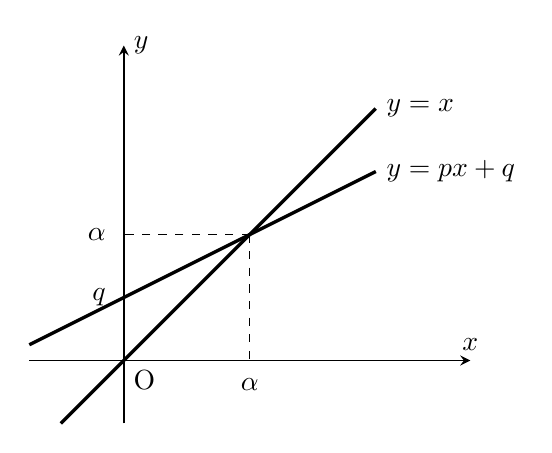
\begin{tikzpicture}[scale=0.8]
    \draw[->,>=stealth,semithick] (-1.5,0)--(5.5,0)node[above]{$x$};
    \draw[->,>=stealth,semithick] (0,-1)--(0,5)node[right]{$y$};
    \draw (0,0)node[below right]{O};

    \draw[very thick,domain=-1:4]
      plot(\x,\x)node[right]{$y=x$};

    \draw[very thick,domain=-1.5:4]
      plot(\x,\x/2+1) node[right] {$y=px+q$};

    % q
    \node[left=3pt] at (0,1) {$q$};

    % 交点から各軸へ点線
    \draw[dashed] (2,2) -- (2,0);
    \draw[dashed] (2,2) -- (0,2);

    % α
    \node[below=3pt] at (2,0) {$\alpha$};
    \node[left=3pt] at (0,2) {$\alpha$};
  \end{tikzpicture}
  \begin{center}
    \BookFigureCaption{直線の交点として捉える\bookterm{fixed}{不動点}}
  \end{center}

  というような状況である.
  この交点$(\alpha,\alpha)$を原点と思ってグラフをみると,この座標平面は$y=px$と$y=x$のグラフが原点から始まって進んでいくようなものに見える.
  言い換えれば等比型\bookterm{recurrence}{漸化式}に帰着させたということである.
  この交点の$x$座標$\alpha$が,更新$f$の\bookterm{fixed}{不動点}である.

  この\bookterm{fixed}{不動点}を知ることによって,複雑な値の変化をより簡素な値の変化に置き換えることができる.
  また,この話から,\,$|p|>1$のときは一般に項数を重ねるにつれて$p$が生み出す等比的な増大が支配的になる一方,\,$|p|<1$のときは$a_n$は$n\to\infty$で$\alpha=\dfrac{q}{1-p}$に収束し,その\bookterm{limit}{極限}値は$q$(と$p$)によって決まることが分かる.例題(2)(\,$p=\frac12$)が$4$に収束するのはこのためである.

  また,\bookterm{characteristic}{特性方程式}型\bookterm{recurrence}{漸化式}には別の解法が存在する.
  以下に示す.
  \begin{align*}
    &a_{n+1}=pa_n+q \tag*{\(\cdots\) (1)}\\
    &a_{n+2}=pa_{n+1}+q \tag*{\(\cdots\) (2)}\\
  \end{align*}
  $(2)-(1)$をし
  \[
    a_{n+2}-a_{n+1}=p(a_{n+1}-a_n)
  \]
  ここで,\,$b_n=a_{n+1}-a_n$と置くと,
  \begin{align*}
    &b_{n+1}=pb_n
  \end{align*}
  このようにすることで,\bookterm{recurrence}{漸化式}は\bookterm{geometric}{等比数列}に帰着する.
  得られた差を初項から足し戻すと、元の\bookterm{sequence}{数列}が求まる。

  こちらの図形的解釈は先程の交点を考えるものとは違う.傾き$p$の平行な2直線$y=px$と$y=px+q$の間には,常に高さ$q$の差が生じている.\,(2)から(1)を引く操作は,この共通の$q$だけを打ち消す操作に対応している.つまり隣接する2つの式を「ずらして引く」ことで,\,$a_n$に無関係な定数項$q$だけを消してしまうのである.これは付録\sectionref{節：差分から始まる離散的な微積分}で扱う\bookterm{difference-operator}{差分}の考え方と同じ発想である.
  これらの前提を元に図示すると

  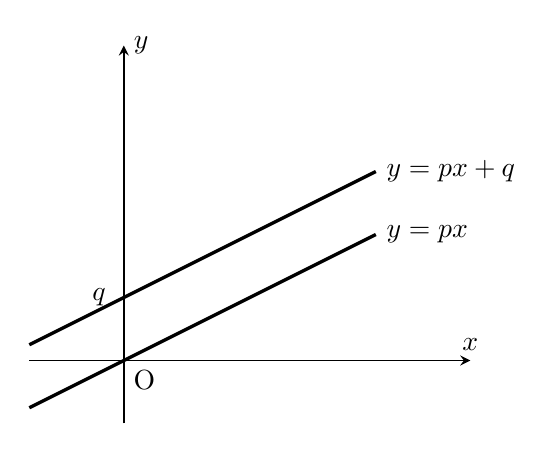
\begin{tikzpicture}[scale=0.8]
    \draw[->,>=stealth,semithick] (-1.5,0)--(5.5,0)node[above]{$x$};
    \draw[->,>=stealth,semithick] (0,-1)--(0,5)node[right]{$y$};
    \draw (0,0)node[below right]{O};

    \draw[very thick,domain=-1.5:4]
      plot(\x,\x/2)node[right]{$y=px$};

    \draw[very thick,domain=-1.5:4]
      plot(\x,\x/2+1) node[right] {$y=px+q$};

    % q
    \node[left=3pt] at (0,1) {$q$};

  \end{tikzpicture}
  \begin{center}
    \BookFigureCaption{定数項の違いを表す平行な直線}
  \end{center}

  常に関数の差が$q$と一定になっていることが図からわかる.

  なお,先ほどの等比的な増大について,初項を\bookterm{fixed}{不動点}に選んだ場合は例外になる.
  \bookterm{fixed}{不動点}から出発すれば値は変わらず,\,$a_n=\alpha$という定\bookterm{sequence}{数列}になるからである.
  式で確かめると,\,$p\ne1$のときは
  \[
    a_n-\alpha=(a_1-\alpha)p^{n-1}
  \]
  である.したがって,\,$|p|>1$でも$a_1=\alpha$ならずれは常に$0$であり,\,$a_1\ne\alpha$の場合に\bookterm{fixed}{不動点}からのずれの絶対値が等比的に増大する.

  今後,\bookterm{characteristic}{特性方程式}を用いた解法を多数扱う.
  \bookterm{characteristic}{特性方程式}は\bookterm{recurrence}{漸化式}を解く中で重要な概念なのである.
  その背景には\bookterm{matrix}{行列}や\bookterm{linear}{線形}代数が深く絡んでいる.

% subsection: 階差等比複合型 \, $\displaystyle a_{n+1}=pa_n+f(n)$

\subsection{\texorpdfstring{階差等比複合型 \, $\displaystyle a_{n+1}=pa_n+f(n)$}{階差等比複合型}}\label{節：階差等比複合型}
  \begin{bookpoint}
    \textbf{同じ更新をする量を引く}\par
    付加項を消すことを目標に,引く式の形と係数を決める.候補を見つける計算と,候補が元の式を満たす確認を区別しよう.
  \end{bookpoint}
  \subsubsection{\texorpdfstring{多項式型 \, $\displaystyle a_{n+1}=pa_n+f(n)$}{多項式型}}
    \bookstep{式の形から、追う量を選ぶ}
    \sectionref*{節：特性方程式型}では,同じ更新をする定数を引いた.
    今回は付加項$f(n)$が$n$によって変わるため,引く量も$n$によって変えてみる.
    \sectionref*{節：補助数列の設計}で述べた方針に従い,同じ更新をする既知の量を探そう.
    本文では$f(n)$が多項式の場合を考える.$p=1$なら\bookterm{difference}{階差}型として和を求められるので,まず$p\ne1$とする.

    \bookstep{引く量を選ぶ}
    $b_n=a_n-g(n)$を等比型にするための条件は
    \[
      g(n+1)=pg(n)+f(n)
    \]
    である.これは,\,$g(n)$自身にも同じ更新をさせるという条件である.
    条件が満たされれば,
    \[
      \begin{array}{rrl}
        &a_{n+1}={}&pa_n+f(n)\\
        -\,)&g(n+1)={}&pg(n)+f(n)\\ \hline
        &a_{n+1}-g(n+1)={}&p\{a_n-g(n)\}
      \end{array}
    \]
    となり,付加項が消える.
    \sectionref*{節：非同次と解の組合せ}で見た「一つの既知の解と\bookterm{homogeneous}{同次}の解に分ける」考え方が,
    ここでは$a_n=g(n)+b_n$として現れている.
    $g(n)$を見つける計算と,残る\bookterm{homogeneous}{同次}の解$b_n$を\bookterm{initial}{初期条件}から選ぶ計算を分けているのである.

    $f(n)$が$m$次式なら,\,$p\ne1$のときは$m$次の多項式
    \[
      g(n)=x_0+x_1n+\cdots+x_mn^m
    \]
    を候補にする.$g(n+1)-pg(n)$の最高次の係数は$(1-p)x_m$である.
    これを$f(n)$の最高次の係数に合わせ,次に一段低い係数を合わせる.
    $1-p\ne0$なので,この順に$x_m,x_{m-1},\ldots,x_0$を決められる.
    未知の係数を比較して求めるこの方法を\bookterm{undetermined}{未定係数法}という.

    例えば$a_{n+1}=2a_n+n-1$では,\,$g(n)=un+v$と置くと
    \[
      u=2u+1,\qquad u+v=2v-1
    \]
    となるので,\,$g(n)=-n$である.
    従って$a_n+n$が2倍される量となる.
    この例の計算は\bookproblemref{practice-basic}{4}{標準問4}で確認する.

    \bookstep{変化を求めて、元の項へ戻す}
    $b_{n+1}=pb_n$を解き,\,$a_n=b_n+g(n)$へ戻す.
    $p\ne0,1$なら
    \[
      a_n=\{a_1-g(1)\}p^{n-1}+g(n)
    \]
    となる.$p=0$なら直接$n\ge2$で$a_n=f(n-1)$と求める.
    一方,\,$p=1$で$f(n)$が$m$次なら,付加項を足し戻す多項式は通常$m+1$次になる.
    例えば$a_{n+1}=a_n+n$では,\,$g(n)=\frac{n(n-1)}2$が同じ更新を満たす.

  \subsubsection{\texorpdfstring{指数型  \, $\displaystyle a_{n+1}=pa_n+q^n$}{指数型}}
    前節では$f(n)$が多項式である場合を扱った.
    ここでは$f(n)$が特に指数関数である場合を扱う.
    指数関数である場合にはもう一つ別の解法が存在する.
    \begin{align*}
      a_{n+1}=pa_n+q^n
    \end{align*}
    以下では$q\ne0$とする($q=0$なら$n\ge1$で$q^n=0$なので等比型になる).
    両辺を$q^n$で割って,
    \begin{align*}
      &\frac{a_{n+1}}{q^n}=\frac{p}{q}\cdot\frac{a_n}{q^{n-1}}+1\\
    \end{align*}
    ここで,\,$b_n=\frac{a_n}{q^{n-1}}$と置くと
    \begin{align*}
      &b_{n+1}=\frac{p}{q}b_n+1
    \end{align*}
    あとは\bookterm{characteristic}{特性方程式}型の\bookterm{recurrence}{漸化式}として解くことになる.
    ただし$p=q$のときは$b_{n+1}=b_n+1$(\bookterm{arithmetic}{等差数列})になり,\bookterm{fixed}{不動点}$\alpha$が存在しない(\sectionref{節：特性方程式型}の例題(3)と同じ状況である).
    この場合は$b_n=b_1+(n-1)$として直接求まる.
    例えば$a_1=1,\,a_{n+1}=2a_n+2^n$(\,$p=q=2$)ならば$b_n=\dfrac{a_n}{2^{n-1}}$が\bookterm{arithmetic}{等差数列}となり,\,$a_n=n\cdot2^{n-1}$が得られる.

% subsection: 対数型 \, $a_{n+1}=pa_n^q$

\subsection{対数型 \, $a_{n+1}=pa_n^q$}
  今までは$a_n$に対する操作は定数倍したり関数が掛けられたりするだけだった.
  しかし,\,$a_n$に指数がついたらどうだろうか.
  この場合はかなり難しい発想の変形が必要である.
  それは対数を取るという操作である.
  実際にやってみよう.
  \[
    a_{n+1}=pa_n^q
  \]
  ただし,対数を取るために$a_n>0$とし,底に選ぶ$p$も$p>0,\,p\ne1$を満たすとする.
  この式について,両辺の対数を取ると
  \begin{align*}
    \log_p{a_{n+1}}&=\log_p{pa_n^q}\\
    &=\log_p{p}+\log_p{a_n^q}\\
    &=q\log_p{a_n}+1
  \end{align*}
  $b_n=\log_p{a_n}$とおくと,
  \begin{align*}
    b_{n+1}=qb_n+1
  \end{align*}
  あとはただの特性方程式型の問題である.
  底をいくらにするかは自由だが$p$に関連する数だと扱いやすい.
  たとえば$p=k^m$の時は$k$でとっておくことが多い.
  作問者側は解答がシンプルな形になるようにするため,より小さい底を取ることで答えが求めやすくなる.

  また,対数の強みは積を和に,商を差にできるところにある.
  漸化式が全て積や商のみで表される場合にその強みが現れる.
  これはここで解説するよりも演習問題を通して経験するほうがわかりやすいと判断したため,この内容は(2)で取り扱っている.

  \noindent\textbf{【例題】}
  \begin{enumerate}[label=(\arabic*),parsep=3pt]
    \item $\displaystyle a_1=2,\quad a_{n+1}=2a_n^2$
    \item $\displaystyle a_1=\frac{1}{2},\quad a_{n+1}=\frac{1}{a_n}$
    \item $\displaystyle a_1=1,\quad a_{n+1}=2^na_n$
    \item $\displaystyle a_1=5,\quad a_{n+1}=a_n^2-2a_n+2$
    \item $\displaystyle a_1=2,\quad a_{n+1}=\frac{a_n^2}{2^n}$
    \item $\displaystyle a_1=1,\quad a_{n+1}=(n+1)a_n$
  \end{enumerate}

  \noindent\textbf{【方針】}
  \begin{enumerate}[label=(\arabic*),parsep=3pt]
    \item 両辺の底を$2$とする対数を取り,\,$b_n=\log_2a_n$とおいて一次の漸化式に変形します.その結果,漸化式は特性方程式型になります.
    \item 一見すると分数型(後述)のように見えますが,対数型として解くことができます.
    \item $f(n)=2^n$が指数関数なので,対数を取ると和の形に帰着できます.
    \item うまく変形すると対数型になります.
    \item 両辺の対数を取ると,二次の漸化式が一次の漸化式に変わり,さらに等差数列の和を使って解くことができます.
    \item 階比型に見えますが,対数型としても解けます.
  \end{enumerate}

  \noindent\textbf{【解答】}
  \begin{enumerate}[label=(\arabic*),parsep=3pt]
    \item $\displaystyle a_n=2^{2^{n}-1}$
    \item $a_n=2^{(-1)^{n}}$
    \item $a_n=2^{\frac{n(n-1)}{2}}$
    \item $a_n=2^{2^n}+1$
    \item $\displaystyle a_n=2^{n-1}-n+1$
    \item $a_n=n!$
  \end{enumerate}

  \noindent\textbf{【解法】}
  \begin{enumerate}[label=(\arabic*),parsep=3pt]
    \item $\displaystyle a_1=2,\quad a_{n+1}=2a_n^2$\\
          両辺の底を$2$とする対数を取ると,
          \begin{align*}
            \log_2a_{n+1}
              &=\log_2{2a_n^2}\\
              &=\log_2{2}+\log_2{a_n^2}\\
              &=2\log_2{a_n}+1
          \end{align*}
          ここで
          \[
            b_n=\log_2a_n
          \]
          とおくと,
          \begin{align*}
            &b_{n+1}=2b_n+1\\
            &b_{n+1}+1=2(b_n+1)
          \end{align*}
          ここで
          \[
            c_n=b_n+1
          \]
          とおくと,
          \[
            c_{n+1}=2c_n
          \]
          $c_1$は,
          \[
            c_1=b_1+1=\log_2{a_1}+1=\log_2{2}+1=1+1=2
          \]
          従って,
          \begin{align*}
            &c_n=2\cdot2^{n-1}=2^n\\
            &b_n+1=2^n\\
            &b_n=2^n-1\\
            &a_n=2^{2^{n}-1}
          \end{align*}
    \item $\displaystyle a_1=\frac12,\quad a_{n+1}=\frac{1}{a_n}$\\
          与式の両辺の底を2とする対数を取ると,
          \begin{align*}
            &\log_2{a_{n+1}}=\log_2{\frac{1}{a_n}}\\
            &\log_2{a_{n+1}}=\log_2{1}-\log_2{a_n}\\
            &\log_2{a_{n+1}}=-\log_2{a_n}\\
            &\log_2{a_n}=\log_2{a_1}(-1)^{n-1}\\
            &\log_2{a_n}=\log_2{\frac{1}{2}}(-1)^{n-1}\\
            &\log_2{a_n}=(-1)^{n}\\
            &\therefore \quad a_n=2^{(-1)^{n}}
          \end{align*}
    \item $\displaystyle a_1=1,\quad a_{n+1}=2^na_n$\\
          両辺の自然対数を取ると
          \[
            \log a_{n+1}=n\log2+\log a_n
          \]
          したがって
          \begin{align*}
            \log a_n&=\log a_1+\sum_{k=1}^{n-1} k\log2\\
            &=\frac{(n-1)n}{2}\log2\\
            &\therefore \quad a_n=2^{\frac{n(n-1)}{2}}
          \end{align*}
    \item $\displaystyle a_1=5,\quad a_{n+1}=a_n^2-2a_n+2$\\
          与式を変形して
          \[
            a_{n+1}-1=(a_n-1)^2
          \]
          両辺の底を2とする対数を取ると,
          \begin{align*}
            &\log_2{(a_{n+1}-1)}=\log_2{(a_n-1)^2}\\
            &\log_2{(a_{n+1}-1)}=2\log_2{(a_n-1)}\\
            &\log_2{(a_n-1)}=2^{n-1}\cdot\log_2{(a_1-1)}\\
            &\log_2{(a_n-1)}=2^{n-1}\cdot\log_2{4}\\
            &\log_2{(a_n-1)}=2^{n}\\
            &a_n-1=2^{2^{n}}\\
            &\therefore \quad a_n=2^{2^{n}}+1
          \end{align*}
    \item $\displaystyle a_1=2,\quad a_{n+1}=\frac{a_n^2}{2^n}$\\
          両辺を底を2とする自然体数を取って
          \[
            equation
          \]
    \item $\displaystyle a_1=1,\quad a_{n+1}=(n+1)a_n$\\
          両辺の自然対数を取って,
          \[
            \log a_{n+1}=\log{n+1}+\log a_n
          \]
          したがって
          \begin{align*}
            \log a_n&=\log a_1 + \log{2}+\cdots+ \log{n}\\
            &=\log 1 + \log{2}+\cdots +\log{n}\\
            &=\log n!\\
            &\therefore \quad a_n=n!
          \end{align*}
  \end{enumerate}
  \noindent\textbf{【補足】}

  (3)では底を自然対数としたが,底は任意の値で構わない.


% parent file: 分数型
\subsection{分数型}\label{節：分数型}
\begin{bookpoint}
  \textbf{分母を簡単にする量を選ぶ}\par
  逆数,または\bookterm{fixed}{不動点}からの二つの差の比を追う.
  分母が零になる初期値と定数解の分岐を確かめてから,置き換えを使う.
\end{bookpoint}
% subsubsection: 逆数型  \, $\displaystyle a_{n+1}=\frac{pa_n}{qa_n+r}$

\subsubsection{\texorpdfstring{逆数型  \, $\displaystyle a_{n+1}=\frac{pa_n}{qa_n+r}$}{逆数型}}
    では逆数型の漸化式について扱っていこう.
    分子が$a_n$の定数倍であることに注目する.
    逆数を取れば,分母にあった一次式を$a_n$で割り,定数と$\frac1{a_n}$の和に分けられる.
    以下では,$p\ne0$かつ$a_n\ne0$であり,$qa_n+r\ne0$として議論する.
    実際に見せよう.
    \begin{align*}
      &a_{n+1}=\frac{pa_n}{qa_n+r}
    \end{align*}
      両辺の逆数を取って
    \begin{align*}
      &\frac{1}{a_{n+1}}=\frac{qa_n+r}{pa_n}\\
      &\frac{1}{a_{n+1}}=\frac{q}{p}+\frac{r}{p}\cdot\frac{1}{a_n}
    \end{align*}
    $\displaystyle \frac{1}{a_n}=b_n$と置くと
    \begin{align*}
      &b_{n+1}=\frac{r}{p}b_n+\frac{q}{p}
    \end{align*}
    このようにすることで,特性方程式型の漸化式に帰着できる.

    \noindent \bookblocklink{example-reciprocal-1}{problem}{answer}{【例題】}
    \begin{enumerate}[label=(\arabic*),parsep=3pt,format=\bookitemlink{example-reciprocal-1}{problem}{answer}]
      \item $\displaystyle a_1=1,\, a_{n+1}=\frac{a_n}{a_n+1}$
      \item $\displaystyle a_1=1,\, a_{n+1}=\frac{-a_n}{2a_n+1}$
    \end{enumerate}

    \noindent\bookblocklink{example-reciprocal-1}{hint}{problem}{【方針】}
    \begin{enumerate}[label=(\arabic*),parsep=3pt,format=\bookitemlink{example-reciprocal-1}{hint}{problem}]
      \item とにかく基本に忠実に解きましょう.
      \item 逆数を取って一次の漸化式に帰着させましょう.
    \end{enumerate}

    \noindent\bookblocklink{example-reciprocal-1}{answer}{problem}{【解答】}
    \begin{enumerate}[label=(\arabic*),parsep=3pt,format=\bookitemlink{example-reciprocal-1}{answer}{problem}]
      \item $\displaystyle a_n=\frac{1}{n}$
      \item $\displaystyle a_n=\frac{1}{2(-1)^{n-1}-1}$
    \end{enumerate}

    \noindent\bookblocklink{example-reciprocal-1}{solution}{problem}{【解法】}
    \begin{enumerate}[label=(\arabic*),parsep=3pt,format=\bookitemlink{example-reciprocal-1}{solution}{problem}]
      \item $\displaystyle a_1=1,\, a_{n+1}=\frac{a_n}{a_n+1}$\\
            両辺の逆数を取って,
            \begin{align*}
              &\frac{1}{a_{n+1}}=\frac{a_n+1}{a_n}=1+\frac{1}{a_n}
            \end{align*}
            $b_n=\dfrac{1}{a_n}$と置くと
            \begin{align*}
              &b_{n+1}=b_n+1,\quad b_1=\frac{1}{a_1}=1\\
              &\therefore \quad b_n=1+(n-1)\cdot1=n\\
              &\therefore \quad a_n=\frac{1}{b_n}=\frac{1}{n}
            \end{align*}
      \item $\displaystyle a_1=1,\, a_{n+1}=\frac{-a_n}{2a_n+1}$\\
            両辺の逆数を取って,
            \begin{align*}
              &\frac{1}{a_{n+1}}=\frac{2a_n+1}{-a_n}=-2-\frac{1}{a_n}
            \end{align*}
            $b_n=\dfrac{1}{a_n}$と置くと,
            \begin{align*}
              &b_{n+1}=-b_n-2,\quad b_1=1
            \end{align*}
            特性方程式型として$\alpha$を求めると,
            \[
              \alpha=-\alpha-2 \ \Leftrightarrow\ \alpha=-1
            \]
            なので,\,$c_n=b_n+1$と置くと,
            \begin{align*}
              &c_{n+1}=-c_n,\quad c_1=b_1+1=2\\
              &\therefore \quad c_n=2\cdot(-1)^{n-1}\\
              &\therefore \quad b_n=c_n-1=2(-1)^{n-1}-1\\
              &\therefore \quad a_n=\frac{1}{b_n}=\frac{1}{2(-1)^{n-1}-1}
            \end{align*}
    \end{enumerate}

% subsubsection: 1次分数型  \, $\displaystyle a_{n+1}=\frac{pa_n+q}{ra_n+s}$

\subsubsection{\texorpdfstring{1次分数型  \, $\displaystyle a_{n+1}=\frac{pa_n+q}{ra_n+s}$}{1次分数型}}\label{節：1次分数型}
    先程の逆数型の一般化と言える漸化式である,\,1次分数型の漸化式について考えていこう.
    以下では,\, $r\ne0$,\, $ps-qr\ne0$とし,もとの漸化式の分母が$0$にならないものとして議論を進める.

    数学における基本的な指針として,既知の形に帰着させるというものがある.
    本書で言う,"きれい"な形にするということである.
    今回の漸化式で,分子の定数項$q$がなければ,つまりは,
    \[
      a_{n+1}=\frac{pa_n+q}{ra_n+s} \Leftrightarrow b_{n+1}=\frac{tb_n}{u b_n+v}
    \]
    となるような$b_n$と$t,u,v$の組があれば逆数型として解くことができる.
    そこで,分子の定数項を消し,逆数型に帰着させることを目標にしよう.

    \,\sectionref{節：特性方程式型}では,数列の各項から同じ定数を引くことで定数項を消した.
    今回もそのアイデアを使い,\, $b_n=a_n-\alpha$と置いてみよう.
    ただし,ここでは$\alpha$をまだ決めず,変形後の分子の定数項が消えるように選ぶ.
    $a_n=b_n+\alpha$を代入すると,
    \begin{align*}
      b_{n+1}-\alpha &=\frac{p(b_n+\alpha)+q}{r(b_n+\alpha)+s}\\
      b_{n+1} &=\frac{p(b_n+\alpha)+q}{r(b_n+\alpha)+s}-\alpha\\
      &=\frac{p(b_n+\alpha)+q-\alpha\{r(b_n+\alpha)+s\}}
        {r(b_n+\alpha)+s}\\
      &=\frac{(p-r\alpha)b_n+p\alpha+q-r\alpha^2-s\alpha}
        {rb_n+r\alpha+s}
    \end{align*}
    となる.したがって,
    \[
      p\alpha+q-r\alpha^2-s\alpha=0
    \]
    となるように$\alpha$を選べば,
    \[
      b_{n+1}=\frac{(p-r\alpha)b_n}{rb_n+r\alpha+s}
    \]
    という逆数型に帰着できる.
    定数項を消すための条件は,
    \[
      r\alpha^2+(s-p)\alpha-q=0
      \quad\Longleftrightarrow\quad
      \alpha=\frac{p\alpha+q}{r\alpha+s}
    \]
    と書けるので,この$\alpha$はもとの漸化式の不動点でもある.
    なお,\, $r\alpha+s=0$なら上の方程式から$p\alpha+q=0$も成り立ち,\, $ps-qr=0$となって仮定に反するので,この分母は$0$ではない.

    ここまでで逆数型として解くことができるが,定数項を消せる値を求める問題は,
    \[
      rx^2+(s-p)x-q=0
    \]
    という二次方程式を解く問題に帰着した.
    この方程式が異なる2つの実数解$\alpha,\beta$を持つなら,その左辺は
    \[
      rx^2+(s-p)x-q=r(x-\alpha)(x-\beta)
    \]
    と因数分解できる.
    $\alpha,\beta$は別々に選ぶ定数ではなく,もとの漸化式の係数から決まる,同じ二次方程式の二つの解なのである.
    そして,どちらの解も定数項を消す条件を満たすので,\, $a_n-\alpha$と$a_n-\beta$のどちらについても,同じ変形ができる.
    先ほどの逆数型の式を,もとの$a_n$を使って書き直すと,
    \begin{align*}
      a_{n+1}-\alpha
      &=\frac{p-r\alpha}{ra_n+s}(a_n-\alpha),\\
      a_{n+1}-\beta
      &=\frac{p-r\beta}{ra_n+s}(a_n-\beta)
    \end{align*}
    となる.

    この二つの式から,さらに単純な法則を取り出せないだろうか.
    それぞれの差に掛かる倍率には$a_n$が含まれているので,差そのものは一般には等比数列にならない.
    しかし,二つの倍率には同じ分母$ra_n+s$が現れている.
    そこで二つの式の比を取れば,この分母が消え,一定の倍率だけが残りそうである.

    初項が$\alpha$または$\beta$なら定数数列になるので,先に扱っておこう.
    以下では初項がどちらの不動点とも異なる場合を考える.
    また,\, $p-r\beta=0$なら不動点の条件から$q=s\beta$となり,\, $ps-qr=0$となって仮定に反する.
    よって,\, $p-r\beta\ne0$であり,上の式から$a_n\ne\beta$なら$a_{n+1}\ne\beta$である.
    初項から順に考えると,すべての項で$a_n\ne\beta$なので,二つの差の比を取ることができる.
    実際に,
    \begin{align*}
      \frac{a_{n+1}-\alpha}{a_{n+1}-\beta}
      &=\cfrac{\displaystyle
        \frac{(p-r\alpha)(a_n-\alpha)}{ra_n+s}}
        {\displaystyle
        \frac{(p-r\beta)(a_n-\beta)}{ra_n+s}}\\
      &=\frac{p-r\alpha}{p-r\beta}
        \frac{a_n-\alpha}{a_n-\beta}
    \end{align*}
    となる.
    したがって,二つの差の比は,項が一つ進むごとに一定の倍率$\dfrac{p-r\alpha}{p-r\beta}$で変化する.
    分子の定数項を消せる二つの式を比べることで,等比数列の法則を見つけられたのである.

    ここで
    \[
      b_n=\frac{a_n-\alpha}{a_n-\beta}
    \]
    と置けば,
    \[
      b_{n+1}
      =
      \frac{p-r\alpha}{p-r\beta}b_n
    \]
    となる.したがって,\,$b_n$は等比数列である.
    $\alpha$と$\beta$の大小関係は,解の大小関係を要求されていないことから自由に選んでよい.
    つまり,\,1次分数型漸化式では,
    \[
      a_{n+1}=\frac{pa_n+q}{ra_n+s}
    \]
    という複雑な形をそのまま扱うのではなく,
    \[
      \frac{a_n-\alpha}{a_n-\beta}
    \]
    という「$\alpha,\beta$からの距離の比」に置き換えることで,
    等比数列に変えることができる.

    そして,\,$\alpha,\beta$は,
    \[
      rx^2+(s-p)x-q=0
    \]
    の異なる2解として自然に現れる.
    
    したがって\,$\alpha,\beta$は,もとの漸化式の$a_n$を形式的に$\alpha,\beta$に置き換えたときにも値が変化しない数,すなわち不動点である.
    
    議論が長くなったので,ここで解法をまとめておこう.
    \[
      a_{n+1}=\frac{pa_n+q}{ra_n+s} 
    \]
    の形で表される漸化式に対して,ただし$ps-qr\ne0$とし,
    $r\ne0$とする.また,以下では$a_n\ne-\dfrac sr$(漸化式の分母が$0$にならないこと)を仮定する.
    さらに,$a_1\ne\beta$とする.
    \[
      x= \frac{px+q}{rx+s} \Leftrightarrow rx^2+(s-p)x-q=0
    \]
    を解き,その異なる2解を$\alpha,\beta$とする.
    ここで,
    \[
      b_n=\frac{a_n-\alpha}{a_n-\beta}
    \]
    と置く.
    すると,
    \begin{align*}
      b_{n+1}&=\frac{a_{n+1}-\alpha}{a_{n+1}-\beta}\\
      &=\cfrac{\displaystyle\frac{pa_n+q}{ra_n+s}-\alpha}{\displaystyle\frac{pa_n+q}{ra_n+s}-\beta}\\
      &=\frac{pa_n+q-\alpha(ra_n+s)}{pa_n+q-\beta(ra_n+s)}\\
      &=\frac{(p-r\alpha)a_n+q-s\alpha}{(p-r\beta)a_n+q-s\beta}
    \end{align*}
    ここで,\,$\alpha$は
    \[
      r\alpha^2+(s-p)\alpha-q=0
    \]
    を満たすから,
    \[
      q-s\alpha=-\alpha(p-r\alpha)
    \]
    である.
    したがって,
    \[
      (p-r\alpha)a_n+q-s\alpha
      =(p-r\alpha)(a_n-\alpha)
    \]
    同様に,\,$\beta$について
    \[
      (p-r\beta)a_n+q-s\beta
      =(p-r\beta)(a_n-\beta)
    \]
    である.
    よって,
    \begin{align*}
      b_{n+1}&=\frac{(p-r\alpha)(a_n-\alpha)}{(p-r\beta)(a_n-\beta)}\\
      &=\frac{p-r\alpha}{p-r\beta}\frac{a_n-\alpha}{a_n-\beta}\\
      &=\frac{p-r\alpha}{p-r\beta}b_n
    \end{align*}
    したがって,
    \[
      b_{n+1}=\frac{p-r\alpha}{p-r\beta}b_n
    \]
    となり,\,$b_n$は等比数列である.
    初項
    \[
      b_1=\frac{a_1-\alpha}{a_1-\beta}
    \]
    を用いれば,
    \[
      b_n=\frac{a_1-\alpha}{a_1-\beta}\left(\frac{p-r\alpha}{p-r\beta}\right)^{n-1} \tag*{\(\cdots\) (＊)}
    \]
    となる.
    最後に,
    \[
      b_n=\frac{a_n-\alpha}{a_n-\beta}
    \]
    から$a_n$を求める.
    \begin{align*}
      b_n(a_n-\beta)&=a_n-\alpha\\
      (b_n-1)a_n&=\beta b_n-\alpha\\
      a_n=\frac{\beta b_n-\alpha}{b_n-1}
    \end{align*}
    (＊)を代入して$a_n$を求めることができる.

    なお,$rx^2+(s-p)x-q=0$が重解$\alpha$を持つ場合は,$\beta$と異なる2つの不動点を取れないため,上の議論はそのまま使えない.
    このときは$\alpha=\dfrac{p-s}{2r}$,すなわち$s=p-2r\alpha$が成り立つため,
    \[
      c=p-r\alpha=r\alpha+s\ne0
    \]
    とおくと,
    \[
      a_{n+1}-\alpha
      =\frac{c(a_n-\alpha)}{r(a_n-\alpha)+c}
    \]
    となる.したがって,
    \[
      \frac{1}{a_{n+1}-\alpha}
      =\frac{1}{a_n-\alpha}+\frac{r}{c}
    \]
    であるから,右辺も含めて$\displaystyle \frac{1}{a_n-\alpha}$について考えれば等差数列に帰着できる.
    ここで$b_n=a_n-\alpha$とおくと,
    \[
      b_{n+1}=\frac{cb_n}{rb_n+c}
    \]
    という逆数型漸化式に帰着する(先ほどの一般式で$\beta=\alpha$とした場合に対応する).したがって両辺の逆数を取れば
    \[
      \frac1{b_{n+1}}=\frac1{b_n}+\frac rc
    \]
    という等差数列が得られ,ここから$a_n$を求めることができる(具体的な計算は例題(3)を参照).

    \noindent \bookblocklink{example-mobius-1}{problem}{answer}{【例題】}
    \begin{enumerate}[label=(\arabic*),parsep=3pt,format=\bookitemlink{example-mobius-1}{problem}{answer}]
      \item $\displaystyle a_1=3,\, a_{n+1}=\frac{2a_n+1}{a_n+2}$
      \item $\displaystyle a_1=0,\, a_{n+1}=\frac{a_n+4}{a_n+1}$
      \item $\displaystyle a_1=5,\, a_{n+1}=\dfrac{4a_{n}-9}{a_{n}-2}$
      \item $\displaystyle a_1=1,\, a_{n+1}=1+\frac{1}{a_n}$
    \end{enumerate}

    \noindent\bookblocklink{example-mobius-1}{hint}{problem}{【方針】}
    \begin{enumerate}[label=(\arabic*),parsep=3pt,format=\bookitemlink{example-mobius-1}{hint}{problem}]
      \item 最も基本的な例です.先程の議論に倣って解きましょう.
      \item 同様に不動点$\alpha,\beta$を求めましょう.今回は片方が負の値になります.
      \item 今回は不動点の方程式が重解になります.\,$\dfrac{a_n-\alpha}{a_n-\beta}$は使えないので,\,$b_n=a_n-\alpha$と置いてから逆数型に帰着させる別の手法を使います.
      \item このような形も一次分数型です.解と係数の関係を活用して解きましょう.
    \end{enumerate}

    \noindent\bookblocklink{example-mobius-1}{answer}{problem}{【解答】}
    \begin{enumerate}[label=(\arabic*),parsep=3pt,format=\bookitemlink{example-mobius-1}{answer}{problem}]
      \item $\displaystyle a_n=\frac{2\cdot3^{n-1}+1}{2\cdot3^{n-1}-1}$
      \item $\displaystyle a_n=\frac{2\left(3^{n-1}+(-1)^n\right)}{3^{n-1}-(-1)^n}$
      \item $a_{n}=\dfrac{6n-1}{2n-1}$
      \item $\displaystyle a_n=\cfrac{\left(\cfrac{1-\sqrt{5}}{2}\right)^{n+1}-\left(\cfrac{1+\sqrt{5}}{2}\right)^{n+1}}{\left(\cfrac{1-\sqrt{5}}{2}\right)^n-\left(\cfrac{1+\sqrt{5}}{2}\right)^n}$
    \end{enumerate}

    \noindent\bookblocklink{example-mobius-1}{solution}{problem}{【解法】}
    \begin{enumerate}[label=(\arabic*),parsep=3pt,format=\bookitemlink{example-mobius-1}{solution}{problem}]
      \item $\displaystyle a_1=3,\, a_{n+1}=\frac{2a_n+1}{a_n+2}$\\
            不動点の方程式は
            \[
              x=\frac{2x+1}{x+2}
            \]
            であるから,その解をそれぞれ$\alpha,\beta$とすると\,$\alpha=1,\ \beta=-1$と取れる.
            このとき,
            \[
              b_n=\frac{a_n-1}{a_n+1}
            \]
            と置くと,
            \begin{align*}
              b_{n+1}&=\frac{a_{n+1}-1}{a_{n+1}+1}\\
              &=\cfrac{\cfrac{2a_n+1}{a_n+2}-1}{\cfrac{2a_n+1}{a_n+2}+1}\\
              &=\frac{2a_n+1-(a_n+2)}{2a_n+1+(a_n+2)}\\
              &=\frac{a_n-1}{3a_n+3}\\
              &=\frac{1}{3}\cdot \frac{a_n-1}{a_n+1}
            \end{align*}
            $\displaystyle b_1=\frac{a_1-1}{a_1+1}=\frac{2}{4}=\frac{1}{2}$から,
            \begin{align*}
              b_{n}=\frac{1}{2}\cdot\left(\frac{1}{3}\right)^{n-1}\\
              \therefore \quad b_n=\frac{1}{2\cdot3^{n-1}}
            \end{align*}
            最後に
            \[
              b_n=\frac{a_n-1}{a_n+1}
            \]
            を$a_n$について解くと,
            \begin{align*}
              &b_n(a_n+1)=a_n-1\\
              &(b_n-1)a_n=-1-b_n\\
              &a_n=\frac{1+b_n}{1-b_n}
            \end{align*}
            \[
              b_n=\frac{1}{2\cdot3^{n-1}}
            \]
            を代入して整理すれば,
            \[
              a_n=\frac{2\cdot3^{n-1}+1}{2\cdot3^{n-1}-1}
            \]
            を得る.
      \item $\displaystyle a_1=0,\, a_{n+1}=\frac{a_n+4}{a_n+1}$\\
            不動点の方程式は
            \[
              x=\frac{x+4}{x+1}
            \]
            であるから,その解をそれぞれ$\alpha,\beta$とすると\,$\alpha=2,\ \beta=-2$と取れる.
            このとき,
            \[
              \frac{p-r\alpha}{p-r\beta}=\frac{1-2}{1+2}=-\frac13
            \]
            なので,
            \[
              b_n=\frac{a_n-2}{a_n+2}
            \]
            と置くと,
            \begin{align*}
              &b_{n+1}=-\frac13 b_n,\quad b_1=\frac{a_1-2}{a_1+2}=\frac{-2}{2}=-1\\
              &\therefore \quad b_n=(-1)\left(-\frac13\right)^{n-1}=\frac{(-1)^n}{3^{n-1}}
            \end{align*}
            \[
              b_n=\frac{a_n-2}{a_n+2}
            \]
            を$a_n$について解くと,
            \[
              a_n=\frac{2(1+b_n)}{1-b_n}
            \]
            となるので,
            \[
              b_n=\frac{(-1)^n}{3^{n-1}}
            \]
            を代入し,分母分子に$3^{n-1}$を掛けて整理すると,
            \[
              a_n=\frac{2\left(3^{n-1}+(-1)^n\right)}{3^{n-1}-(-1)^n}
            \]
            を得る.
      \item $\displaystyle a_1=5,\, a_{n+1}=\dfrac{4a_{n}-9}{a_{n}-2}$
            不動点の方程式は
            \[
              x=\frac{4x-9}{x-2}
            \]
            であるから,その解は3.
            \[
            b_n=a_n-3
            \]
            とおくと,
            \begin{align*}
              b_{n+1}&=a_{n+1}-3\\
              &=\dfrac{4a_{n}-9}{a_{n}-2}-3\\
              &=\dfrac{a_{n}-3}{a_{n}-2}\\
              &=\dfrac{b_{n}}{b_{n}+1}
            \end{align*}
            逆数を取って
            \begin{align*}
              \frac{1}{b_{n+1}}&=\dfrac{b_{n}+1}{b_{n}}
            \end{align*}
            $b_1=a_1-3=2$,すなわち$\dfrac1{b_1}=\dfrac12$より,
            \begin{align*}
              &\frac{1}{b_n}=\frac{1}{2}+(n-1)\cdot 1\\
              &\frac{1}{b_n}=\frac{2n-1}{2}\\
              &b_n=\frac{2}{2n-1}\\
              &a_n-3=\frac{2}{2n-1}\\
              &a_n=\frac{6n-1}{2n-1}
            \end{align*}
      \item $\displaystyle a_1=1,\, a_{n+1}=1+\frac{1}{a_n}$\\
            式を変形して
            $\displaystyle a_1=1,\, a_{n+1}=\frac{a_n+1}{a_n}$
            不動点の方程式は
            \[
              x=\frac{x+1}{x}\tag*{\(\cdots\) (1)}
            \]
            であるから,その解をそれぞれ$\alpha,\beta$とすると
            \[
              \alpha=\frac{1+\sqrt{5}}{2},\ \beta=\frac{1-\sqrt{5}}{2}
            \]
            ここで(1)について,その解$\alpha,\beta$では
            \[
              \alpha+\beta=1,\, \quad \alpha\beta=-1\tag*{\(\cdots\) (2)}
            \]
            が解と係数の関係から成り立つ.したがって,
            \begin{align*}
              b_{n+1}&=\frac{a_{n+1}-\alpha}{a_{n+1}-\beta}\\
              &=\cfrac{\cfrac{a_n+1}{a_n}-\alpha}{\cfrac{a_n+1}{a_n}-\beta}\\
              &=\frac{a_n+1-\alpha a_n}{a_n+1-\beta a_n}\\
              &=\frac{(1-\alpha)a_n+1}{(1-\beta)a_n+1}\tag*{\(\cdots\) (3)}
            \end{align*}
            (2)より,(3)は
            \begin{align*}
              \frac{(1-\alpha)a_n+1}{(1-\beta)a_n+1}&=\frac{\beta a_n+1}{\alpha a_n+1}\\
              &=\frac{\beta a_n-\alpha\beta}{\alpha a_n-\alpha\beta}\\
              &=\frac{\beta (a_n-\alpha)}{\alpha (a_n-\beta)}\\
              &=\frac{\beta}{\alpha}b_n
            \end{align*}
            よって,
            \[
              b_{n+1}=\frac{\beta}{\alpha}b_n
            \]
            初項$b_1$は,
            \begin{align*}
              b_1=\frac{a_1-\alpha}{a_1-\beta}=\frac{1-\alpha}{1-\beta}=\frac{\beta}{\alpha}
            \end{align*}
            したがって,
            \[
              b_n=\left(\frac{\beta}{\alpha}\right)^n
            \]
            次に
            \[
              b_{n}=\frac{a_{n}-\alpha}{a_{n}-\beta}
            \]
            を$a_n$について解くと,
            \[
              a_{n}=\frac{\beta b_{n}-\alpha}{b_{n}-1}
            \]
            したがって,
            \begin{align*}
              a_{n}&=\cfrac{\beta \left(\cfrac{\beta}{\alpha}\right)^n-\alpha}{\left(\cfrac{\beta}{\alpha}\right)^n-1}  \\
              &=\frac{\beta^{n+1}-\alpha^{n+1}}{\beta^n-\alpha^n}\\
              &=\cfrac{\left(\cfrac{1-\sqrt{5}}{2}\right)^{n+1}-\left(\cfrac{1+\sqrt{5}}{2}\right)^{n+1}}{\left(\cfrac{1-\sqrt{5}}{2}\right)^n-\left(\cfrac{1+\sqrt{5}}{2}\right)^n}
            \end{align*}        
    \end{enumerate}
  余談にはなるが,最後の問題はフィボナッチ数列の2項間の比の極限値は黄金比$\dfrac{1+\sqrt{5}}{2}$に一致する.
  実際,\,$a_n=\dfrac{F_{n+1}}{F_n}$(ただし$F_n$は$F_1=F_2=1$から定まるフィボナッチ数列)であることが,同じ漸化式$a_{n+1}=1+\dfrac1{a_n}$から確かめられる.
  また,ここから派生したリュカ数列も同じ特性方程式$x^2=x+1$を持ち,隣接項の比が同じ黄金比に収束する.
  一方,同様に漸化式から派生する数列にトリボナッチ数列があるが,こちらは特性方程式が3次$(x^3=x^2+x+1)$になり,隣接項の比の極限値(トリボナッチ定数,約$1.839$)は黄金比とは異なる.
  これらは本書の趣旨から外れてしまうため割愛する.

  加えて,このタイプの漸化式は帰納法によって示すことが比較的容易なパターンが存在する.
  例えば(3)は解答の一般項から分かるように,分母分子それぞれが一次関数の形で書かれているため,想像しやすい.
  $a_1$から$a_3$ぐらいまでを求めさせてから帰納法で示させるような誘導問題が出た時は帰納法を使って解くことも視野に入れておくといいだろう.
  以下にその例を示す.\\
    \noindent\bookblocklink{example-mobius-2}{problem}{answer}{【例題】}
    \begin{quote}
      以下の漸化式
      \[
        a_1=5,\, a_{n+1}=\dfrac{4a_{n}-9}{a_{n}-2}
      \]
      を満たす数列$a_n$の一般項を帰納法を用いて求めよ.
    \end{quote}
    \bookblocklink{example-mobius-2}{hint}{problem}{【方針】}
    \begin{quote}
      実験的に代入計算をしてみると,
      \[
        a_1=\frac{5}{1},\,a_2=\frac{11}{3},\,a_3=\frac{17}{5},\,a_4=\frac{23}{7},\,a_5=\frac{29}{9}
      \]
      となる.分母が2ずつ,分子が6づつ増えていることから,一般項は
      \[
        a_n=\frac{6n-1}{2n-1}
      \]
      と予想する.
    \end{quote}
    \bookblocklink{example-mobius-2}{answer}{problem}{【解答】}
    \begin{quote}
      一般項$a_n$が
      \[
        a_n=\frac{6n-1}{2n-1}
      \]
      であることを示す.\\
      $n=1$の時,
      \[
        \frac{6-1}{2-1}=5
      \]
      よって成立する.\\
      ある正の整数$k$について,$n=k$が成り立つと仮定する.このとき,
      \[
        n=k+1
      \]
      のとき,
      \begin{align*}
        a_{k+1}&=\frac{4a_{k}-9}{a_{k}-2}\\
        &=\cfrac{4\cdot \cfrac{6k-1}{2k-1}-9}{\cfrac{6k-1}{2k-1}-2}\\
        &=\frac{4(6k-1)-9(2k-1)}{6k-1-2(2k-1)}\\
        &=\frac{6k+5}{2k+1}\\
        &=\frac{6(k+1)-1}{2(k+1)-1}
      \end{align*}
      したがって,$n=k+1$でも成立する.
      以上より
      \[
        a_n=\frac{6n-1}{2n-1}
      \]
      が示された.\qed

  \end{quote}


% subsubsection: 極形式による図形的解釈

\subsubsection{極形式による図形的解釈}
  \BookFigMobius

  図では,点$a_n$と二つの\bookterm{fixed}{不動点}$\alpha,\beta$を結ぶ線分を描いた.
  上の線分の長さを下の線分の長さで割ると,
  \[
    \frac{|a_n-\alpha|}{|a_n-\beta|}
    =\left|\frac{a_n-\alpha}{a_n-\beta}\right|
    =|b_n|
  \]
  となる.また,二つの線分の向きの差は,
  $b_n$の\bookterm{argument}{偏角}$\arg b_n$に対応する.
  したがって,図で見ている\textbf{長さの比と角度の差}は,
  計算で導入する一つの複素数$b_n$の絶対値と\bookterm{argument}{偏角}に他ならない.
  さらに$b_{n+1}=\lambda b_n$となったときは,
  長さの比が$|\lambda|$倍され,角度の差が$\arg\lambda$だけ増える.
  特に$|\lambda|=1$なら,長さの比を保ったまま\bookterm{argument}{偏角}だけが変わり,
  \bookterm{complex-plane}{複素平面}上の回転として理解できる.


  ここまででは,\,$\alpha,\beta$を\bookterm{fixed}{不動点}として
  \[
    b_n=\frac{a_n-\alpha}{a_n-\beta}
  \]
  と置くことで,1次分数型の\bookterm{recurrence}{漸化式}を\bookterm{geometric}{等比数列}に帰着できることを示した.

  ここでは,この変形を\bookterm{complex-plane}{複素平面}上で考えてみよう.
  まず注意したいのは,
  \[
    \frac{a_n-\alpha}{a_n-\beta}
  \]
  そのものを「距離の比」と呼ぶのは正確ではないという点である.
  実数上でも符号の情報を含み,\bookterm{complex-plane}{複素平面}上では\bookterm{argument}{偏角}の情報まで含む.
  実際に距離の比を表すのは絶対値を取った
  \[
    \left|\frac{a_n-\alpha}{a_n-\beta}\right|
    =
    \frac{|a_n-\alpha|}{|a_n-\beta|}
  \]
  であり,これは点$a_n$から$\alpha,\beta$までの距離の比である.
  一方,もとの複素数の比には,この距離の比に加えて二つの差の\bookterm{argument}{偏角}の差も記録されている.

  特に,\,$\alpha,\beta$が実数ではなく複素数となる場合には,この変形によって\bookterm{recurrence}{漸化式}を「回転」として解釈することができる.

  $p,q,r,s$が実数であるとき,
  \[
    rx^2+(s-p)x-q=0
  \]
  の2解が実数でなければ,解と係数の関係から,2解は互いに\bookterm{conjugate}{共役}な複素数となる.
  そこで,その2解を
  \[
    \beta=\overline{\alpha}
  \]
  とする.

  このとき,
  \[
    b_n=\frac{a_n-\alpha}{a_n-\overline{\alpha}}
  \]
  と置くと,先ほどと同じ変形によって
  \[
    b_{n+1}
    =
    \frac{p-r\alpha}{p-r\overline{\alpha}}b_n
  \]
  となる.

  ここで,
  \[
    \lambda=\frac{p-r\alpha}{p-r\overline{\alpha}}
  \]
  とおく.
  \, $p,r$は実数であり,\,$\overline{p-r\alpha}=p-r\overline{\alpha}$であるから,
  \[
    |\lambda|
    =
    \left|
    \frac{p-r\alpha}{p-r\overline{\alpha}}
    \right|
    =1
  \]
  である.

  したがって,\,$\lambda$は\bookterm{polar}{極形式}を用いて
  \[
    \lambda=\cos\theta+i\sin\theta
  \]
  と表すことができる.

  一方,\,$b_n$も\bookterm{polar}{極形式}を用いて
  \[
    b_n=\rho_n(\cos\varphi_n+i\sin\varphi_n)
  \]
  と表すことができる.
  このとき,
  \begin{align*}
    b_{n+1}
    &=
    (\cos\theta+i\sin\theta)
    \rho_n(\cos\varphi_n+i\sin\varphi_n)\\
    &=
    \rho_n
    \{\cos(\varphi_n+\theta)
    +i\sin(\varphi_n+\theta)\}
  \end{align*}
  であるから,
  \[
    \rho_{n+1}=\rho_n,
    \qquad
    \varphi_{n+1}=\varphi_n+\theta
  \]
  となる.

  つまり,$b_n$は\bookterm{complex-plane}{複素平面}上で原点からの距離を変えずに,\,$\theta$だけずつ回転している.

  このことから,
  \[
    b_{n+1}=\lambda b_n
  \]
  という\bookterm{geometric}{等比数列}への帰着は,単なる計算上の技巧ではなく,\bookterm{complex-plane}{複素平面}上の図形的な変化を表していることが分かる.

  実際に,次の\bookterm{recurrence}{漸化式}を考えてみよう.
  \[
    a_{n+1}=\frac{a_n+1}{1-a_n}
  \]
  この\bookterm{recurrence}{漸化式}の\bookterm{fixed}{不動点}は
  \[
    x=\frac{x+1}{1-x}
  \]
  を解けばよいから,
  \[
    x^2+1=0
  \]
  より
  \[
    \alpha=i,\qquad\beta=-i
  \]
  である.

  そこで,
  \[
    b_n=\frac{a_n-i}{a_n+i}
  \]
  と置くと,
  \begin{align*}
    b_{n+1}
    &=
    \frac{1+i}{1-i}b_n
  \end{align*}
  となる.

  ここで,
  \[
    \frac{1+i}{1-i}
    =
    \frac{(1+i)^2}{2}
    =i
  \]
  であるから,
  \[
    b_{n+1}=ib_n
  \]
  を得る.

  $i$は\bookterm{polar}{極形式}で
  \[
    i=\cos\frac{\pi}{2}+i\sin\frac{\pi}{2}
  \]
  と表せる.
  したがって,\,$b_n$は\bookterm{complex-plane}{複素平面}上で毎回反時計回りに$\dfrac{\pi}{2}$だけ回転する.

  例えば,\,$a_1=\dfrac12$とすると,
  \begin{align*}
    a_1&=\frac12\\
    a_2&=3\\
    a_3&=-2\\
    a_4&=-\frac13\\
    a_5&=\frac12
  \end{align*}
  となり,\,$a_n$は
  \[
    \frac12\longrightarrow3\longrightarrow-2
    \longrightarrow-\frac13\longrightarrow\frac12\longrightarrow\cdots
  \]
  と変化する.

  一方,\,$b_n$に着目すると,
  \[
    b_{n+1}=ib_n
  \]
  であるから,
  \[
    b_1\longrightarrow ib_1\longrightarrow-b_1
    \longrightarrow-ib_1\longrightarrow b_1\longrightarrow\cdots
  \]
  となる.

  つまり,実数上では複雑に見える
  \[
    a_1,a_2,a_3,\ldots
  \]
  の変化が,
  \[
    b_n=\frac{a_n-i}{a_n+i}
  \]
  という変換によって,\bookterm{complex-plane}{複素平面}上で一定角度ずつ回転する点の運動として表される.

  このように,異なる二つの\bookterm{fixed}{不動点}をもつ1次分数型\bookterm{recurrence}{漸化式}では,
  \[
    \frac{a_n-\alpha}{a_n-\beta}
  \]
  という変換を用いることで,\bookterm{recurrence}{漸化式}を\bookterm{geometric}{等比数列}に変形できる.
  特に,係数が実数で\bookterm{fixed}{不動点}が非実の\bookterm{conjugate}{共役}な二点であるときには,変換後の点の変化を\bookterm{complex-plane}{複素平面}上の回転として図形的に解釈することができる.


% subsection: 隣接3項間漸化式型 \, $\displaystyle a_{n+2}+pa_{n+1}+qa_n=0$

\subsection{\texorpdfstring{隣接3項間漸化式型 \, $\displaystyle a_{n+2}+pa_{n+1}+qa_n=0$}{隣接3項間漸化式型}}\label{節：隣接3項間漸化式型}
  \BookFigThreeTerm

  \subsubsection{\texorpdfstring{二次特性方程式型 \, $\displaystyle a_{n+2}+pa_{n+1}+qa_n=0$}{二次特性方程式型}}\label{節：二次特性方程式型}
    節は変われど,特性方程式を使って考える.
    結局,大方の場合,等比数列に変形できればいいのだから,これを等比数列に変形できないかといくつかの試行錯誤を重ねるのが王道の解き方である.
    結果から言ってしまえば,特性方程式型のところで少し触れた式を生み出すことで等比数列を作ることができる.
    \[
      a_{n+2}+pa_{n+1}+qa_n=0
    \]
    について,
    \[
      a_{n+2}-\alpha a_{n+1}=\beta(a_{n+1}-\alpha a_{n})
    \]
    となるような$\alpha,\beta$の組を探せば良い.
    変形すると
    \begin{align*}
      &a_{n+2}-\alpha a_{n+1}=\beta(a_{n+1}-\alpha a_{n})\\
      &\therefore \quad a_{n+2}-(\alpha+\beta)a_{n+1}+\alpha\beta a_n=0
    \end{align*}
    である.これが元の漸化式
    \[
      a_{n+2}+pa_{n+1}+qa_n=0
    \]
    と一致するには,
    \[
      \alpha+\beta=-p,\quad \alpha\beta=q
    \]
    であればよい.これは解と係数の関係そのものであるから,\,$\alpha,\beta$は
    \[
      x^2+px+q=0
    \]
    の2解として得られる.

    \,$x^2+px+q=0$の2解を$\alpha,\beta$とすると,元の漸化式は
    \[
      \begin{cases}
        a_{n+1}-\alpha a_n=\beta(a_n-\alpha a_{n-1})\\
        a_{n+1}-\beta a_n=\alpha(a_n-\beta a_{n-1})
      \end{cases}
    \]
    という2つの等比数列を生む(添字は1つずれているが本質的には先程と同じ議論である).

    $\alpha\ne\beta$の時,
    \[
      b_n=a_{n+1}-\alpha a_n
    \]
    は公比$\beta$の等比数列であるから,
    \[
      b_n=b_1\beta^{n-1}
    \]
    である.ここで,
    \[
      b_1=a_2-\alpha a_1
    \]
    なので,
    \[
      a_{n+1}-\alpha a_n
      =(a_2-\alpha a_1)\beta^{n-1}
    \]
    を得る.

    同様に,
    \[
      c_n=a_{n+1}-\beta a_n
    \]
    は公比$\alpha$の等比数列であるから,
    \[
      c_n=c_1\alpha^{n-1}
    \]
    である.また,
    \[
      c_1=a_2-\beta a_1
    \]
    なので,
    \[
      a_{n+1}-\beta a_n
      =(a_2-\beta a_1)\alpha^{n-1}
    \]
    となる.

    ここで,この2式から$a_{n+1}$を消去するために,上の式から下の式を引くと,
    \begin{align*}
      &(a_{n+1}-\alpha a_n)-(a_{n+1}-\beta a_n)\\
      &\qquad=(a_2-\alpha a_1)\beta^{n-1}
      -(a_2-\beta a_1)\alpha^{n-1}
    \end{align*}
    である.左辺を整理すると,
    \[
      (\beta-\alpha)a_n
      =(a_2-\alpha a_1)\beta^{n-1}
      -(a_2-\beta a_1)\alpha^{n-1}.
    \]
    $\alpha\ne\beta$より$\beta-\alpha\ne0$であるから,
    \[
      a_n
      =\frac{a_2-\alpha a_1}{\beta-\alpha}\beta^{n-1}
      -\frac{a_2-\beta a_1}{\beta-\alpha}\alpha^{n-1}
    \]
    となる.

    ここで,\,$a_1,a_2,\alpha,\beta$は$n$によらない定数であるから,係数をまとめれば,
    \[
      a_n=A\alpha^{n-1}+B\beta^{n-1}
    \]
    と書くことができる.
    これは\sectionref*{節：解を組み合わせる見方}で学んだ,二つの解の線形結合である.
    非零の異なる根なら,$\alpha^{n-1}$と$\beta^{n-1}$の初めの二項は$(1,\alpha)$と$(1,\beta)$であり,
    一次独立なので基底になる.係数$A,B$を初期条件で選ぶことは,2次元の解全体から一つを選ぶことに当たる.
    \,$\alpha=\beta$(重解)の場合は上の議論がそのままは使えないため,別に扱う.
    同じ冪を二つ並べても一次独立にはならないので,別の形の解が必要になる.
    このときは$b_n=a_{n+1}-\alpha a_n$のみを考え,\,$b_{n+1}=\alpha b_n$という等比数列に帰着させてから,さらに階差型または等比複合型として解く(具体的な手順は例題(2)を参照).

    \noindent \bookblocklink{example-three-term-1}{problem}{answer}{【例題】}
    \begin{enumerate}[label=(\arabic*),parsep=3pt,format=\bookitemlink{example-three-term-1}{problem}{answer}]
      \item $\displaystyle a_1=1,\,a_2=1,\, a_{n+2}=5a_{n+1}-6a_n$
      \item $\displaystyle a_1=1,\,a_2=4,\, a_{n+2}=4a_{n+1}-4a_n$
      \item $\displaystyle a_1=2,\,a_2=1,\, a_{n+2}=a_{n+1}+6a_n$
    \end{enumerate}

    \noindent\bookblocklink{example-three-term-1}{hint}{problem}{【方針】}
    \begin{enumerate}[label=(\arabic*),parsep=3pt,format=\bookitemlink{example-three-term-1}{hint}{problem}]
      \item 特性方程式$x^2-5x+6=0$の解は異なる2つの実数解です.素直に2本の等比数列を作りましょう.
      \item 特性方程式$x^2-4x+4=0$を解くと重解になります.等比数列は1本しか作れないことに注意しましょう.
      \item 特性方程式の解の1つが負になるパターンです.符号に注意して計算しましょう.
    \end{enumerate}

    \noindent\bookblocklink{example-three-term-1}{answer}{problem}{【解答】}
    \begin{enumerate}[label=(\arabic*),parsep=3pt,format=\bookitemlink{example-three-term-1}{answer}{problem}]
      \item $\displaystyle a_n=2^n-3^{n-1}$
      \item $\displaystyle a_n=n\cdot2^{n-1}$
      \item $\displaystyle a_n=(-2)^{n-1}+3^{n-1}$
    \end{enumerate}

    \noindent\bookblocklink{example-three-term-1}{solution}{problem}{【解法】}
    \begin{enumerate}[label=(\arabic*),parsep=3pt,format=\bookitemlink{example-three-term-1}{solution}{problem}]
      \item $\displaystyle a_1=1,\,a_2=1,\, a_{n+2}=5a_{n+1}-6a_n$\\
            特性方程式
            \[
              x^2-5x+6=0
            \]
            を解くと,
            \[
              (x-2)(x-3)=0
            \]
            より$\alpha=2,\beta=3$である.
            \begin{align*}
              &a_{n+2}-2a_{n+1}=3(a_{n+1}-2a_n)\\
              &a_{n+2}-3a_{n+1}=2(a_{n+1}-3a_n)
            \end{align*}
            なので
            \[
              b_n=a_{n+1}-2a_n,\,c_n=a_{n+1}-3a_n
            \]
            と置くと,
            \begin{align*}
              &b_n=b_1\cdot3^{n-1},\quad b_1=a_2-2a_1=-1\\
              &c_n=c_1\cdot2^{n-1},\quad c_1=a_2-3a_1=-2\\
              &\therefore \quad b_n=-3^{n-1},\quad c_n=-2^n
            \end{align*}
            したがって
            \[
              b_n-c_n=(a_{n+1}-2a_n)-(a_{n+1}-3a_n)=a_n
            \]
            であるから,
            \[
              a_n=-3^{n-1}-(-2^n)=2^n-3^{n-1}
            \]
      \item $\displaystyle a_1=1,\,a_2=4,\, a_{n+2}=4a_{n+1}-4a_n$\\
            特性方程式
            \[
              x^2-4x+4=0
            \]
            を解くと,
            \[
              (x-2)^2=0
            \]
            より$\alpha=2$である.
            \[
              b_n=a_{n+1}-2a_n
            \]
            と置くと,
            \begin{align*}
              b_{n+1}&=a_{n+2}-2a_{n+1}\\
              &=(4a_{n+1}-4a_n)-2a_{n+1}\\
              &=2(a_{n+1}-2a_n)\\
              &=2b_n
            \end{align*}
            また,
            \begin{align*}
              b_1=a_2-2a_1=2
            \end{align*}
            から,
            \[
              b_n=2\cdot2^{n-1}=2^n
            \]
            したがって
            \[
              a_{n+1}-2a_n=2^n
            \]
            である.両辺を$2^{n+1}$で割ると,
            \[
              \frac{a_{n+1}}{2^{n+1}}-\frac{a_n}{2^n}=\frac12
            \]
            ここで
            \[
              c_n=\dfrac{a_n}{2^n}
            \]
            と置くと,
            \begin{align*}
              &c_{n+1}=c_n+\frac12,\quad c_1=\frac{a_1}{2}=\frac12\\
              &\therefore \quad c_n=\frac12+(n-1)\cdot\frac12=\frac n2\\
              &\therefore \quad a_n=2^n\cdot c_n=n\cdot2^{n-1}
            \end{align*}
      \item $\displaystyle a_1=2,\,a_2=1,\, a_{n+2}=a_{n+1}+6a_n$\\
            特性方程式
            \[
              x^2-x-6=0
            \]
            を解くと,
            \[
              (x-3)(x+2)=0
            \]
            より$\alpha=3,\beta=-2$である.
            \begin{align*}
              &a_{n+2}-3a_{n+1}=-2(a_{n+1}-3a_n)\\
              &a_{n+2}+2a_{n+1}=3(a_{n+1}+2a_n)
            \end{align*}
            なので,
            \[
              b_n=a_{n+1}-3a_n,\ c_n=a_{n+1}+2a_n
            \]
            と置くと,
\BookMathLayout{\begin{align*}
              &b_n=b_1\cdot(-2)^{n-1},\quad b_1=a_2-3a_1=-5\\
              &c_n=c_1\cdot3^{n-1},\quad c_1=a_2+2a_1=5\\
              &\therefore \quad b_n=-5(-2)^{n-1},\quad c_n=5\cdot3^{n-1}
            \end{align*}}{
\[
\begin{aligned}
b_n&=b_1\cdot(-2)^{n-1},\\ b_1&=a_2-3a_1=-5\\
c_n&=c_1\cdot3^{n-1},\\ c_1&=a_2+2a_1=5\\
\therefore\quad b_n&=-5(-2)^{n-1},\\ c_n&=5\cdot3^{n-1}
\end{aligned}
\]
}
            \[
              c_n-b_n=(a_{n+1}+2a_n)-(a_{n+1}-3a_n)=5a_n
            \]
            であるから,
            \begin{align*}
              5a_n&=5\cdot3^{n-1}-\{-5(-2)^{n-1}\}\\
              &=5\cdot3^{n-1}+5(-2)^{n-1}\\
              \therefore\quad a_n&=(-2)^{n-1}+3^{n-1}
            \end{align*}
    \end{enumerate}

  \subsubsection{\texorpdfstring{等差二次特性方程式型 \, $\displaystyle a_{n+2}+pa_{n+1}+qa_n=r$}{等差二次特性方程式型}}\label{節：等差二次特性方程式型}
    今度は右辺が0ではなく$r$となった.
    つまり$r$だけズレたのである.
    ズレたらもとに戻す,つまり不動点を探すのである.
    \[
      b_n=a_n-\alpha
    \]
    となる$\alpha$を求めると,
    \begin{align*}
      &(a_{n+2}-\alpha)+p(a_{n+1}-\alpha)+q(a_n-\alpha)=0\\
      &a_{n+2}+pa_{n+1}+qa_n=\alpha+p\alpha+q\alpha\\
      &\therefore \quad r=\alpha +p\alpha +q\alpha\\
      &\Leftrightarrow \quad \alpha=\frac{r}{p+q+1}\quad(p+q+1\ne0)
    \end{align*}
    ただし$p+q+1=0$かつ$r\ne0$のときは定数解$\alpha$が存在しない.\,$p+q+1=0$かつ$r=0$なら任意の定数が条件を満たし,元の漸化式はすでに前節の形である.定数解が存在しない場合は$d_n=a_{n+1}-a_n$とおくと,元の漸化式から$d_{n+1}=qd_n+r$となり,特性方程式型または階差型に帰着できる.
    あとは前節で述べた隣接3項間漸化式の問題である.

    \noindent \bookblocklink{example-three-term-2}{problem}{answer}{【例題】}
    \begin{enumerate}[label=(\arabic*),parsep=3pt,format=\bookitemlink{example-three-term-2}{problem}{answer}]
      \item $\displaystyle a_1=2,\,a_2=2,\, a_{n+2}=5a_{n+1}-6a_n+2$
      \item $\displaystyle a_1=1,\,a_2=2,\, a_{n+2}=4a_{n+1}-4a_n+3$
    \end{enumerate}

    \noindent\bookblocklink{example-three-term-2}{hint}{problem}{【方針】}
    \begin{enumerate}[label=(\arabic*),parsep=3pt,format=\bookitemlink{example-three-term-2}{hint}{problem}]
      \item まず不動点$\alpha$を求め,\,$b_n=a_n-\alpha$と置いて前節の二次特性方程式型に帰着させましょう.
      \item こちらは重解のパターンです.同じ手順で$\alpha$を求めてから前節の重解の場合の処理を行いましょう.
    \end{enumerate}

    \noindent\bookblocklink{example-three-term-2}{answer}{problem}{【解答】}
    \begin{enumerate}[label=(\arabic*),parsep=3pt,format=\bookitemlink{example-three-term-2}{answer}{problem}]
      \item $\displaystyle a_n=1+2^n-3^{n-1}$
      \item $\displaystyle a_n=3+2^{n-2}(3n-7)$
    \end{enumerate}

    \noindent\bookblocklink{example-three-term-2}{solution}{problem}{【解法】}
    \begin{enumerate}[label=(\arabic*),parsep=3pt,format=\bookitemlink{example-three-term-2}{solution}{problem}]
      \item $\displaystyle a_1=2,\,a_2=2,\, a_{n+2}=5a_{n+1}-6a_n+2$
            \begin{align*}
              &a_{n+2}=5a_{n+1}-6a_n+2\\
              &a_{n+2}-5a_{n+1}+6a_n=2
            \end{align*}
            ここで
            \[
              (a_{n+2}-\alpha)-5(a_{n+1}-\alpha)+6(a_n-\alpha)=0 
            \]
            を満たす$\alpha$を求めると,
            \[
              \alpha=1
            \]
            $b_n=a_n-1$と置くと,
            \begin{align*}
              &b_{n+2}=5b_{n+1}-6b_n\\
              &b_1=1,\, b_2=1
            \end{align*}
            （答案中略。先ほどの二次特性方程式型の例題(1)と同じ漸化式に帰着する.全く同じ計算を$b_n$に対して行う）
            \[
              b_n=2^n-3^{n-1}
            \]
            を得るから,
            \[
              a_n=1+b_n=1+2^n-3^{n-1}
            \]
      \item $\displaystyle a_1=1,\,a_2=2,\, a_{n+2}=4a_{n+1}-4a_n+3$
            \begin{align*}
              &a_{n+2}=4a_{n+1}-4a_n+3\\
              &a_{n+2}-4a_{n+1}+4a_n=3
            \end{align*}
            ここで
            \[
              (a_{n+2}-\alpha)-4(a_{n+1}-\alpha)+4(a_n-\alpha)=0 
            \]
            を満たす$\alpha$を求めると,
            \[
              \alpha=3
            \]
            なので,\,$b_n=a_n-3$と置くと,
            \begin{align*}
              &b_{n+2}=4b_{n+1}-4b_n\\
              &b_1=a_1-3=-2\\
              &b_2=a_2-3=-1                
            \end{align*}
            特性方程式$x^2-4x+4=0$は重解$\alpha'=2$を持つから,\,$c_n=b_{n+1}-2b_n$と置くと,
            \begin{align*}
              &c_{n+1}=2c_n\\
              &c_1=b_2-2b_1=-1-2(-2)=3\\
              &\therefore \quad c_n=3\cdot2^{n-1}
            \end{align*}
            したがって$b_{n+1}-2b_n=3\cdot2^{n-1}$である.両辺を$2^{n+1}$で割ると,
            \begin{align*}
              &\frac{b_{n+1}}{2^{n+1}}-\frac{b_n}{2^n}=\frac34
            \end{align*}
            $f_n=\dfrac{b_n}{2^n}$と置くと,
            \begin{align*}
              &f_{n+1}=f_n+\frac34,\quad f_1=\frac{b_1}{2}=-1\\
              &\therefore \quad f_n=-1+(n-1)\cdot\frac34=\frac{3n-7}{4}\\
              &\therefore \quad b_n=2^n\cdot f_n=2^{n-2}(3n-7)
            \end{align*}
            よって,
            \[
              a_n=3+b_n=3+2^{n-2}(3n-7)
            \]
    \end{enumerate}

% subsection: 総和型

\subsection{総和型}
  \subsubsection{総和と一般項の漸化式型 \, $S_n=pa_n+f(n)$}
    ある漸化式によって定められる数列$a_n$によって,
    \[
      S_n=\sum_{k=1}^{n} a_k
    \]
    として定められる数列$S_n$について考えよう.
    $S_n$と$a_n$の関係を表した
    \[
      S_n=pa_n+f(n)
    \]
    のような漸化式を考える.
    このような漸化式は今まで取り扱った形にはない,未知のものである.
    であれば既知の形にするのが数学である.
    これまでのことをきちんと理解していれば,\,$a_{n+1}$と$a_n$の関係が分かっている時には解くことができる.
    $S_n$をうまく変形して$a_{n}$関連だけの式を産むには,\,$p \neq 1$の時,
    \begin{align*}
      &S_n=pa_n+f(n) \tag*{\(\cdots\) (1)}\\
      &S_{n+1}=pa_{n+1}+f(n+1) \tag*{\(\cdots\) (2)}
    \end{align*}
    $(2)-(1)$をして
    \begin{align*}
      &a_{n+1}=pa_{n+1}-pa_n+f(n+1)-f(n)\\
      &a_{n+1}-pa_{n+1}=-pa_n+f(n+1)-f(n)\\
      &a_{n+1}(1-p)=-pa_n+f(n+1)-f(n)\\
      &a_{n+1}=\frac{-pa_n+f(n+1)-f(n)}{(1-p)}\\
      &a_{n+1}=\frac{p}{p-1}a_n+\frac{1}{1-p}\{f(n+1)-f(n)\}
    \end{align*}
    $\displaystyle g(n)=\frac{1}{1-p}\{f(n+1)-f(n)\}$とおくと,
    \begin{align*}
      &a_{n+1}=\frac{p}{p-1}a_n+g(n)
    \end{align*}
    従って漸化式は階差等比複合型(\ref{節：階差等比複合型})に帰着する(係数$\frac{p}{p-1}$は$p=p-1$となることがないため,決して$1$にはならない).
    \,$p=1$のときはこの割り算ができないが,\,$S_n=a_n+f(n)$と$S_n=S_{n-1}+a_n$($n\ge2$)を見比べることで,直接$a_n=f(n+1)-f(n)$が得られる.

    \noindent \textbf{【例題】}
    \begin{enumerate}[label=(\arabic*),parsep=3pt]
      \item $\displaystyle S_n=2a_n-n$
      \item $\displaystyle S_n=\frac12a_n+n$
    \end{enumerate}

    \noindent\textbf{【方針】}
    \begin{enumerate}[label=(\arabic*),parsep=3pt]
      \item まず$n=1$を代入して$a_1$を求めてから,本文の変形をなぞって$a_{n+1}$と$a_n$だけの漸化式を作りましょう.
      \item 同様です.できた漸化式は特性方程式型に帰着します.
    \end{enumerate}

    \noindent\textbf{【解答】}
    \begin{enumerate}[label=(\arabic*),parsep=3pt]
      \item $\displaystyle a_n=2^n-1$
      \item $\displaystyle a_n=1+(-1)^{n-1}$
    \end{enumerate}

    \noindent\textbf{【解法】}
    \begin{enumerate}[label=(\arabic*),parsep=3pt]
    \item $\displaystyle S_n=2a_n-n$

        $n=1$を代入すると,
        \[
          S_1=a_1=2a_1-1
        \]
        より
        \[
          a_1=1
        \]
        また,
        \begin{align*}
          a_{n+1}
            &=S_{n+1}-S_n\\
            &=\{2a_{n+1}-(n+1)\}-(2a_n-n)\\
            &=2a_{n+1}-2a_n-1
        \end{align*}
        したがって,
        \[
          a_{n+1}=2a_n+1
        \]
        ここで $b_n=a_n+1$ とおくと,
        \begin{align*}
          b_{n+1}
            &=a_{n+1}+1\\
            &=2a_n+2\\
            &=2(a_n+1)\\
            &=2b_n
        \end{align*}
        また,
        \[
          b_1=a_1+1=2
        \]
        であるから,
        \[
          b_n=2^n
        \]
        よって,
        \[
          a_n=2^n-1
        \]
    \item $\displaystyle S_n=\frac12a_n+n$
        $n=1$を代入すると,
        \[
          S_1=a_1=\frac12a_1+1
        \]
        より
        \[
          a_1=2
        \]
        \begin{align*}
          a_{n+1}
            &=S_{n+1}-S_n\\
            &=\left\{\frac12a_{n+1}+(n+1)\right\}-\left(\frac12a_n+n\right)\\
            &=\frac12a_{n+1}-\frac12a_n+1
        \end{align*}
        したがって,
        \[
          a_{n+1}=-a_n+2
        \]

        ここで $b_n=a_n-1$ とおくと,
        \begin{align*}
          b_{n+1}
            &=a_{n+1}-1\\
            &=-a_n+1\\
            &=-(a_n-1)\\
            &=-b_n
        \end{align*}
        また,
        \[
          b_1=a_1-1=1
        \]
        であるから,
        \[
          b_n=(-1)^{n-1}
        \]
        よって,
        \[
          a_n=1+(-1)^{n-1}
        \]

    \end{enumerate}

  \subsubsection{純総和型 \, $S_{n+1}=pS_n+f(n) $}
    両辺に総和がきてもやることは一緒で,1つずらした総和と元の式を足し引きしてやることで,\,$a_n$や$a_{n+1}$の項を作れば良い.
    \begin{align*}
      &S_{n+1}=pS_n+f(n) \tag*{\(\cdots\) (1)}\\
      &S_{n}=pS_{n-1}+f(n-1) \tag*{\(\cdots\) (2)}\\
    \end{align*}
      $(1)-(2)$をして,
    \begin{align*}
      &a_{n+1}=pa_{n}+f(n)-f(n-1)
    \end{align*}
    ただし(2)は(1)の$n$を$n-1$に置き換えたものなので,この式は$n\ge2$の範囲でのみ成り立つ.\,$a_1$と$a_2$の関係は,別途$S_1,S_2$から直接求める必要がある.
    あとはただの階差数列型の計算である.

    \noindent \textbf{【例題】}
    \begin{enumerate}[label=(\arabic*),parsep=3pt]
      \item $\displaystyle S_1=1,\ S_{n+1}=2S_n+n$
    \end{enumerate}

    \noindent\textbf{【方針】}
    \begin{enumerate}[label=(\arabic*),parsep=3pt]
      \item 本文の式は$n\ge2$でしか使えないことに注意し,\,$a_2$だけは$S_2=2S_1+f(1)$から別に求めましょう.
    \end{enumerate}

    \noindent\textbf{【解答】}
    \begin{enumerate}[label=(\arabic*),parsep=3pt]
      \item $\displaystyle a_1=1,\quad a_n=3\cdot2^{n-2}-1\ (n\ge2)$
    \end{enumerate}

    \noindent\textbf{【解法】}
    \begin{enumerate}[label=(\arabic*),parsep=3pt]
    \item $\displaystyle S_1=1,\ S_{n+1}=2S_n+n$

        $a_1=S_1=1$である.
        本文で示した公式
        \[
          a_{n+1}=pa_{n}+f(n)-f(n-1)
        \]
        に$p=2,\ f(n)=n$を代入すると,
        \[
          a_{n+1}=2a_n+\{n-(n-1)\}=2a_n+1\quad(n\ge2)
        \]
        を得る(この式は$n\ge2$でのみ成り立つことに注意する).

        実際,\,$n=1$のときは
        \[
          a_2=S_2-S_1=(2S_1+1)-S_1=2
        \]
        であるが,\,$2a_1+1=2\cdot1+1=3\ne a_2$であるから,この漸化式は$a_1$から$a_2$へは使えない.

        そこで,\,$n\ge2$の範囲で $b_n=a_n+1$ とおくと,
        \begin{align*}
          b_{n+1}
            &=a_{n+1}+1\\
            &=2a_n+2\\
            &=2(a_n+1)\\
            &=2b_n\qquad(n\ge2)
        \end{align*}
        また,
        \[
          b_2=a_2+1=3
        \]
        であるから,
        \[
          b_n=3\cdot2^{n-2}\quad(n\ge2)
        \]
        よって,
        \[
          a_1=1,\quad a_n=3\cdot2^{n-2}-1\quad(n\ge2)
        \]
    \end{enumerate}


% subsection: 連立型

\subsection{連立型}\label{節：連立型}
  \subsubsection{加減法型}
    一般形が
    \[
      \begin{cases}
        a_{n+1}=pa_{n}+qb_{n} \\
        b_{n+1}=qa_{n}+pb_{n}
      \end{cases}
    \]
    の形で表される漸化式の解き方について考えよう.
    二つの式では係数$p,q$の位置が入れ替わっている.
    足すと両方の係数が$p+q$になり,引くと$p-q$とその符号反転が現れる.
    そこで,和と差がそれぞれ単独で更新されないか調べる.
    実際にすすめていくと,
    \begin{align*}
      &a_{n+1}+b_{n+1}=(p+q)(a_{n}+b_{n})\\
      &a_n+b_n=(a_1+b_1)(p+q)^{n-1}\tag*{\(\cdots\) (1)}
    \end{align*}
    また,
    \begin{align*}
      &a_{n+1}-b_{n+1}=(p-q)(a_{n}-b_{n})\\
      &a_n-b_n=(a_1-b_1)(p-q)^{n-1}\tag*{\(\cdots\) (2)}
    \end{align*}
    $(1)+(2)$をすると
\BookMathLayout{\begin{align*}
      &2a_n=(a_1+b_1)(p+q)^{n-1}+(a_1-b_1)(p-q)^{n-1}\\
      &a_n=\frac{(a_1+b_1)(p+q)^{n-1}+(a_1-b_1)(p-q)^{n-1}}{2}\\
    \end{align*}}{
\[
\begin{aligned}
2a_n&=(a_1+b_1)(p+q)^{n-1}\\
&\quad+(a_1-b_1)(p-q)^{n-1}\\
a_n&=\frac{1}{2}\bigl\{(a_1+b_1)(p+q)^{n-1}\\
&\qquad+(a_1-b_1)(p-q)^{n-1}\bigr\}
\end{aligned}
\]
}
    $(1)-(2)$をすると
\BookMathLayout{\begin{align*}
      &2b_n=(a_1+b_1)(p+q)^{n-1}-(a_1-b_1)(p-q)^{n-1}\\
      &b_n=\frac{(a_1+b_1)(p+q)^{n-1}-(a_1-b_1)(p-q)^{n-1}}{2}
    \end{align*}}{
\[
\begin{aligned}
2b_n&=(a_1+b_1)(p+q)^{n-1}\\
&\quad-(a_1-b_1)(p-q)^{n-1}\\
b_n&=\frac{1}{2}\bigl\{(a_1+b_1)(p+q)^{n-1}\\
&\qquad-(a_1-b_1)(p-q)^{n-1}\bigr\}
\end{aligned}
\]
}
    \sectionref*{節：一次独立・基底・次元}で,初期条件を独立な二つの解に分けたことを思い出そう.
    ここでは初期の組$(a_1,b_1)$を
    \[
      \begin{aligned}
        (a_1,b_1)
        &=\frac{a_1+b_1}{2}(1,1)\\
        &\quad+\frac{a_1-b_1}{2}(1,-1)
      \end{aligned}
    \]
    と分けた.$(1,1)$から始まる部分は$p+q$倍,$(1,-1)$から始まる部分は$p-q$倍される.
    上の一般項は,二つの解を線形結合して元の初期条件に合わせた式である.
    和と差という補助量を取り出すことが,解を独立な二つの部分に分けることにつながっていた.
    別解及び演習は一般型の方で行う.
  \subsubsection{一般型}
    連立一般型の漸化式は,
    \[
      \begin{cases}
        a_{n+1}=pa_{n}+qb_{n} \\
        b_{n+1}=ra_{n}+sb_{n}
      \end{cases}
    \]
    で表される漸化式である.
    いつものように等比数列型への帰着を目指そう.
    $a_n$と$b_n$が互いに影響し合っているため,独立させて解くことは難しそうだ.
    ならばそれぞれについて求めるのではなく,いっそのこと合わせて求めてしまおうというのが解法の思想である.
    その流れは,
\BookMathLayout{\[
      \begin{array}{rrl}
        & a_{n+1}={} &pa_{n}+qb_{n}\\
        +\,) & b_{n+1}={} & ra_{n}+sb_{n}\\ \hline
        & a_{n+1}+b_{n+1}={} & (p+r)a_{n}+(q+s)b_{n}
      \end{array}
    \]}{
\[
\setlength{\arraycolsep}{2pt}
\begin{array}{rrl}
&a_{n+1}={}&pa_n+qb_n\\
+\,)&b_{n+1}={}&ra_n+sb_n\\\hline
&a_{n+1}+b_{n+1}={}&(p+r)a_n+(q+s)b_n
\end{array}\]
}
    について
    \[
      \alpha a_{n+1}+\beta b_{n+1}
      =\gamma(\alpha a_n+\beta b_n)
    \]
    を満たすようにしてやればよい.
    実際に左辺を計算すると,
\BookMathLayout{\begin{align*}
      \alpha a_{n+1}+\beta b_{n+1}&=\alpha(pa_n+qb_n)+\beta(ra_n+sb_n)\\
      &=(p\alpha+r\beta)a_n+(q\alpha+s\beta)b_n
    \end{align*}}{
\[
\begin{aligned}
\alpha a_{n+1}+\beta b_{n+1}
&=\alpha(pa_n+qb_n)\\ &\quad+\beta(ra_n+sb_n)\\
&=(p\alpha+r\beta)a_n\\ &\quad+(q\alpha+s\beta)b_n
\end{aligned}
\]
}
    一方,
    \[
      \gamma(\alpha a_n+\beta b_n)=\gamma\alpha a_n+\gamma\beta b_n
    \]
    である.
    したがって,
    \[
    \begin{cases}
      p\alpha+r\beta=\gamma\alpha\\
      q\alpha+s\beta=\gamma\beta
    \end{cases}
    \]
    となるように$\alpha,\beta,\gamma$を決めればよい.

    ここで,いきなり3つの文字をすべて求めようとすると少し複雑に見える.
    そこで,まず$\gamma$について考える.

    上の2式を変形すると,
    \[
    \begin{cases}
      (p-\gamma)\alpha+r\beta=0\\
      q\alpha+(s-\gamma)\beta=0
    \end{cases}
    \]
    である.
    $\alpha,\beta$は同時に$0$ではないので,この連立方程式が$\alpha,\beta$について解を持つためには,
    \[
      (p-\gamma)(s-\gamma)-qr=0
    \]
    でなければならない.
    整理すると,
    \[
      \gamma^2-(p+s)\gamma+(ps-qr)=0
    \]
    となる.
    この二次方程式を,この連立漸化式の特性方程式と呼ぶ.
    特性方程式の解を$\gamma_1,\gamma_2$とする.
    まず$\gamma=\gamma_1$を上の連立方程式に代入し,
    \[
      \begin{cases}
        (p-\gamma_1)\alpha+r\beta=0\\
        q\alpha+(s-\gamma_1)\beta=0
      \end{cases}
    \]
    を満たす$\alpha,\beta$を1組求める.
    すると,
    \[
      c_n=\alpha a_n+\beta b_n
    \]
    と置くことで,
    \begin{align*}
      c_{n+1}&=\alpha a_{n+1}+\beta b_{n+1}\\
      &=\gamma_1(\alpha a_n+\beta b_n)\\
      &=\gamma_1c_n
    \end{align*}
    となる.
    したがって,
    \[
      c_n=c_1\gamma_1^{\,n-1}
    \]
    という等比数列が得られる.
    同様に,\,$\gamma=\gamma_2$に対しても$\alpha,\beta$を求めれば,
    \[
      d_n=\alpha' a_n+\beta' b_n
    \]
    について
    \[
      d_n=d_1\gamma_2^{\,n-1}
    \]
    という等比数列が得られる.
    なお,ここで得られた2つの等比数列から$a_n,b_n$を求めるには,
    \[
      \begin{cases}
      c_n=\alpha a_n+\beta b_n\\
      d_n=\alpha'a_n+\beta'b_n
      \end{cases}
    \]
    を$a_n,b_n$について解けばよい.
    ただし,この連立方程式から$a_n,b_n$を一意に求めるには,係数の組$(\alpha,\beta)$と$(\alpha',\beta')$が比例しないこと,すなわち$\alpha\beta'-\alpha'\beta\ne0$が必要である.
    $\gamma_1\ne\gamma_2$ならこの条件を満たすが,これは十分条件であって必要条件ではない.
    重解の場合でも,例えば$a_{n+1}=2a_n,\,b_{n+1}=2b_n$では$(1,0),(0,1)$を選べる.
    一方,重解に対して比例しない2組を取れない場合は,別の工夫が必要になる(\sectionref{節：二次特性方程式型}の重解の場合と同様の考え方を用いる).
    また,$\,\gamma_1,\gamma_2$が虚数になる場合もこの手法は形式的には成り立つが,実数の形に書き直すには\sectionref{節：虚数解型隣接3項間漸化式}で扱う手法が必要になる.
    このように,\,$a_n,b_n$をそれぞれ直接求めるのではなく,\,$a_n,b_n$の和の形を作ることで,連立していた漸化式を等比数列へと分離することができる.

    \noindent \bookblocklink{example-system-1}{problem}{answer}{【例題】}
    \begin{enumerate}[label=(\arabic*),parsep=3pt,format=\bookitemlink{example-system-1}{problem}{answer}]
      \item $\displaystyle a_1=1,\,b_1=1.\ \begin{cases}a_{n+1}=3a_n+b_n\\ b_{n+1}=a_n+3b_n\end{cases}$
      \item $\displaystyle a_1=1,\,b_1=0,\ \begin{cases}a_{n+1}=3a_n+b_n\\ b_{n+1}=2a_n+2b_n\end{cases}$
    \end{enumerate}

    \noindent\bookblocklink{example-system-1}{hint}{problem}{【方針】}
    \begin{enumerate}[label=(\arabic*),parsep=3pt,format=\bookitemlink{example-system-1}{hint}{problem}]
      \item 前節で述べた問題です.一般型,加減法型,どちらのやり方でも問題ありません.
      \item これはこの節で述べたものです.
    \end{enumerate}

    \noindent\bookblocklink{example-system-1}{answer}{problem}{【解答】}
    \begin{enumerate}[label=(\arabic*),parsep=3pt,format=\bookitemlink{example-system-1}{answer}{problem}]
      \item $\displaystyle a_n=4^{n-1},\qquad b_n=a_n=4^{n-1}$
      \item $\displaystyle a_n=\frac{2\cdot4^{n-1}+1}{3},\qquad b_n=\frac{2\cdot4^{n-1}-2}{3}$
    \end{enumerate}

    \noindent\bookblocklink{example-system-1}{solution}{problem}{【解法】}
    \begin{enumerate}[label=(\arabic*),parsep=3pt,format=\bookitemlink{example-system-1}{solution}{problem}]
    \item $\displaystyle a_1=1,\,b_1=1.\ \begin{cases}a_{n+1}=3a_n+b_n\\ b_{n+1}=a_n+3b_n\end{cases}$\\
          \begin{enumerate}
            \item 【解法1】\\
                  $\alpha a_{n+1}+\beta b_{n+1}$を計算すると,
                  \begin{align*}
                    \alpha a_{n+1}+\beta b_{n+1}
                      &=\alpha(3a_n+b_n)\\
                      &\qquad +\beta(a_n+3b_n)\\
                      &=(3\alpha+\beta)a_n\\
                      &\qquad +(\alpha+3\beta)b_n
                  \end{align*}
                  これが
                  \[
                    \gamma(\alpha a_n+\beta b_n)
                    =\gamma\alpha a_n+\gamma\beta b_n
                  \]
                  と一致するためには,
                  \[
                  \begin{cases}
                    (3-\gamma)\alpha+\beta=0\\
                    \alpha+(3-\gamma)\beta=0
                  \end{cases}
                  \]
                  でなければならない.

                  $\alpha,\beta$が同時に$0$ではないため,
                  \[
                    (3-\gamma)^2-1=0
                  \]
                  より,
                  \begin{align*}
                    &\gamma^2-6\gamma+8=0\\
                    &(\gamma-2)(\gamma-4)=0
                  \end{align*}
                  したがって,
                  \[
                    \gamma_1=2,\qquad\gamma_2=4
                  \]
                  である.

                  まず$\gamma=2$とすると,
                  \[
                  \begin{cases}
                    \alpha+\beta=0\\
                    \alpha+\beta=0
                  \end{cases}
                  \]
                  となるので,
                  \[
                    \alpha=1,\qquad\beta=-1
                  \]
                  と取ることができる.

                  そこで,
                  \[
                    c_n=a_n-b_n
                  \]
                  とおくと,
                  \begin{align*}
                    c_{n+1}
                      &=a_{n+1}-b_{n+1}\\
                      &=(3a_n+b_n)-(a_n+3b_n)\\
                      &=2(a_n-b_n)\\
                      &=2c_n
                  \end{align*}
                  また,
                  \[
                    c_1=a_1-b_1=0
                  \]
                  であるから,
                  \[
                    c_n=0
                  \]
                  したがって,
                  \[
                    a_n-b_n=0
                  \]

                  次に$\gamma=4$とすると,
                  \[
                  \begin{cases}
                    -\alpha+\beta=0\\
                    \alpha-\beta=0
                  \end{cases}
                  \]
                  となるので,
                  \[
                    \alpha=1,\qquad\beta=1
                  \]
                  と取ることができる.

                  そこで,
                  \[
                    d_n=a_n+b_n
                  \]
                  とおくと,
                  \begin{align*}
                    d_{n+1}
                      &=a_{n+1}+b_{n+1}\\
                      &=(3a_n+b_n)+(a_n+3b_n)\\
                      &=4(a_n+b_n)\\
                      &=4d_n
                  \end{align*}
                  また,
                  \[
                    d_1=a_1+b_1=2
                  \]
                  であるから,
                  \[
                    d_n=2\cdot4^{n-1}
                  \]

                  以上より,
                  \[
                  \begin{cases}
                    a_n-b_n=0\\
                    a_n+b_n=2\cdot4^{n-1}
                  \end{cases}
                  \]
                  となる.

                  2式を辺々加えると,
                  \[
                    2a_n=2\cdot4^{n-1}
                  \]
                  であるから,
                  \[
                    a_n=4^{n-1}
                  \]
                  また,
                  \[
                    b_n=a_n=4^{n-1}
                  \]
            \item 【解法2】\\
                  2つの式を辺々加えると,
                  \begin{align*}
                    a_{n+1}+b_{n+1}
                      &=(3a_n+b_n)\\
                      &\quad +(a_n+3b_n)\\
                      &=4(a_n+b_n)
                  \end{align*}
                  よって,
                  \[
                    a_n+b_n=(a_1+b_1)4^{n-1}=2\cdot4^{n-1}. \tag*{\(\cdots\) (1)}
                  \]

                  また,2つの式を辺々引くと,
                  \begin{align*}
                    a_{n+1}-b_{n+1}
                      &=(3a_n+b_n)\\
                      &\quad -(a_n+3b_n)\\
                      &=2(a_n-b_n)
                  \end{align*}
                  よって,
                  \[
                    a_n-b_n=(a_1-b_1)2^{n-1}=0. \tag*{\(\cdots\) (2)}
                  \]

                  \((1)+(2)\)をすると,
                  \[
                    2a_n=2\cdot4^{n-1}
                  \]
                  なので,
                  \[
                    a_n=4^{n-1}
                  \]

                  また,\((1)-(2)\)をすると,
                  \[
                    2b_n=2\cdot4^{n-1}
                  \]
                  なので,
                  \[
                    b_n=4^{n-1}
                  \]
          \end{enumerate}
    \item $\displaystyle a_1=1,\,b_1=0,\ \begin{cases}a_{n+1}=3a_n+b_n\\ b_{n+1}=2a_n+2b_n\end{cases}$\\
          $\alpha a_{n+1}+\beta b_{n+1}$を計算すると,
          \begin{align*}
            \alpha a_{n+1}+\beta b_{n+1}
              &=\alpha(3a_n+b_n)\\
              &\quad +\beta(2a_n+2b_n)\\
              &=(3\alpha+2\beta)a_n\\
              &\quad +(\alpha+2\beta)b_n
          \end{align*}
          これが
          \[
            \gamma(\alpha a_n+\beta b_n)
            =\gamma\alpha a_n+\gamma\beta b_n
          \]
          と一致するためには,
          \[
          \begin{cases}
            (3-\gamma)\alpha+2\beta=0\\
            \alpha+(2-\gamma)\beta=0
          \end{cases}
          \]
          でなければならない.

          $\alpha,\beta$が同時に$0$ではないため,
          \[
            (3-\gamma)(2-\gamma)-2=0
          \]
          より,
          \begin{align*}
            &\gamma^2-5\gamma+4=0\\
            &(\gamma-1)(\gamma-4)=0
          \end{align*}
          したがって,
          \[
            \gamma_1=1,\qquad\gamma_2=4
          \]
          である.

          まず$\gamma=1$とすると,
          \[
          \begin{cases}
            2\alpha+2\beta=0\\
            \alpha+\beta=0
          \end{cases}
          \]
          となるので,
          \[
            \alpha=1,\qquad\beta=-1
          \]
          と取ることができる.

          そこで,
          \[
            c_n=a_n-b_n
          \]
          とおくと,
          \begin{align*}
            c_{n+1}
              &=a_{n+1}-b_{n+1}\\
              &=(3a_n+b_n)-(2a_n+2b_n)\\
              &=a_n-b_n\\
              &=c_n
          \end{align*}
          また,
          \[
            c_1=a_1-b_1=1
          \]
          であるから,
          \[
            c_n=1
          \]
          したがって,
          \[
            a_n-b_n=1
          \]

          次に$\gamma=4$とすると,
          \[
          \begin{cases}
            -\alpha+2\beta=0\\
            \alpha-2\beta=0
          \end{cases}
          \]
          となるので,
          \[
            \alpha=2,\qquad\beta=1
          \]
          と取ることができる.

          そこで,
          \[
            d_n=2a_n+b_n
          \]
          とおくと,
          \begin{align*}
            d_{n+1}
              &=2a_{n+1}+b_{n+1}\\
              &=2(3a_n+b_n)+(2a_n+2b_n)\\
              &=8a_n+4b_n\\
              &=4(2a_n+b_n)\\
              &=4d_n
          \end{align*}
          また,
          \[
            d_1=2a_1+b_1=2
          \]
          であるから,
          \[
            d_n=2\cdot4^{n-1}
          \]

          以上より,
          \[
          \begin{cases}
            a_n-b_n=1\\
            2a_n+b_n=2\cdot4^{n-1}
          \end{cases}
          \]
          となる.

          2式を辺々加えると,
          \[
            3a_n=1+2\cdot4^{n-1}
          \]
          であるから,
          \[
            a_n=\frac{2\cdot4^{n-1}+1}{3}
          \]
          また,
          \[
            b_n=a_n-1
          \]
          より,
          \[
            b_n=\frac{2\cdot4^{n-1}-2}{3}
          \]
    \end{enumerate}



% section: 発展パターン

\section{発展パターン}\label{節：発展パターン}
ここでは更に発展的なパターンについて紹介する.
扱われる漸化式は,一部の難関大において時々出題されるようなものである.
基本的に誘導がついた状態で出題されるため,ひと目見て解けるようになる必要はそこまで高くないが,知っていて損はない.
ここで追加する変数係数型は階比型と階差型の組合せ,
二重数列は階差と帰納法を二方向へ広げる見方である.
新しい型名を覚えるだけでなく,既習の操作がどこで働くかを確かめよう.
\subsection{変数係数の一次漸化式}\label{節：変数係数の一次漸化式}
  \sectionref*{節：階比型}では添字ごとの倍率を掛け合わせ,
  \sectionref*{節：階差等比複合型}では同じ更新をする量を引いた.
  ここでは,倍率と付加項がどちらも添字に依存する場合を,この二つの操作で解こう.

  \subsubsection{倍率をそろえて,変化を足す}
  まず
  \BookMathLayout{\[
    a_1=2,\qquad
    a_{n+1}=\frac{n+2}{n}a_n+(n+1)(n+2)
    \quad(n\ge1)
  \]}{\[
    \begin{aligned}
      a_1&=2,\\
      a_{n+1}&=\frac{n+2}{n}a_n+(n+1)(n+2)\\
      &\quad(n\ge1)
    \end{aligned}
  \]}
  を考える.係数の分子・分母に注目すると,
  \[
    \frac{(n+1)(n+2)}{n(n+1)}=\frac{n+2}{n}
  \]
  である.\textbf{隣り合う項の比が元の倍率になる量}として$h_n=n(n+1)$を選べる.
  これは\sectionref*{節：補助数列の設計}で目標から割る量を選んだ方法である.
  $b_n=\frac{a_n}{n(n+1)}$と置いて実際に計算すると,
  \[
    \frac{a_{n+1}}{(n+1)(n+2)}
      =\frac{a_n}{n(n+1)}+1
  \]
  となる.従って$b_1=1$, $b_{n+1}=b_n+1$より$b_n=n$であり,
  \[
    a_n=n^2(n+1)
  \]
  を得る.分母は$n\ge1$で非零である.初項と元の式へ代入しても確かめられる.

  \subsubsection{一般の手順と,割り算の条件}
  $a_{n+1}=p_na_n+q_n$ $(n\ge1)$に対して,
  $h_1=1$, $h_{n+1}=p_nh_n$とする.
  すべての$p_n$が非零なら,$h_n$も非零であり,
  \[
    h_n=\prod_{k=1}^{n-1}p_k
  \]
  である.空積は$1$とする.両辺を$h_{n+1}$で割ると,
  \[
    b_n=\frac{a_n}{h_n},\qquad
    b_{n+1}-b_n=\frac{q_n}{h_{n+1}}
  \]
  だから,階差を足して
  \[
    a_n=h_n\left(a_1+\sum_{k=1}^{n-1}\frac{q_k}{h_{k+1}}\right)
  \]
  を得る.先ほどは定数倍して$h_n=n(n+1)$を選んだが,
  その場合の$b_1$を正しく合わせれば同じ答えになる.

  \begin{bookpoint}
    \textbf{正規化の役割}\par
    倍率を取り除くと,残った付加項を足す問題になる.
    積・和の表示を得ることと,最後まで簡単な式で計算できることは別である.
  \end{bookpoint}
  もし$p_j=0$なら,$a_{j+1}=q_j$はそれ以前の項によらず決まる.
  零を含む$h_n$で割らず,零となる更新の前後で区間を分け,
  非零の倍率が続く範囲で同じ方法を使う.

  \subsubsection{同じ更新をする量を引く別解}
  先ほどの例では,$v_n=n^2(n+1)$が元の更新を満たすことを直接確かめられる.
  この候補は,正規化後の$b_n=n$から見つけたものである.
  $d_n=a_n-v_n$と置くと,
  \[
    d_{n+1}=\frac{n+2}{n}d_n
  \]
  となり,階比型へ戻る.初項を一般の$a_1=s$に変えると,
  \[
    a_n=n(n+1)\left(n+\frac{s-2}{2}\right)
  \]
  である.一つの解$v_n$と,同次の解の定数倍に分かれている.
  これは\sectionref*{節：非同次と解の組合せ}の見方そのものである.

  \begin{bookpoint}
    \textbf{二つの方法の選び方}\par
    隣り合う比が分かるなら割る因子を探す.
    同じ更新をする既知の量が見えるならそれを引く.
    どちらも,付加項と倍率を分けて扱うための操作である.
  \end{bookpoint}
  操作だけの比較は\sectionref*{節：操作を選ぶ練習},
  一般項まで求める練習は\bookproblemref{practice-connections}{1}{接続演習問1}へ進もう.

\subsection{ガウス型}\label{節：ガウス型}
  ここまでの漸化式では,差を取る,定数を引く,別の数列に置き換えるなどの操作から,既知の形へ帰着させてきた.
  ガウス記号を含む場合も,この方針は変わらない.
  ただし,変形の手掛かりとして,整数性,不等式,余り,偶奇,数え上げなどが必要になる.
  ガウス型では,整数問題で用いる考え方が前面に現れるのである.

  ガウス記号があるというだけで,一つの解法が決まるわけではない.
  本項では,\textbf{ガウス記号が式の中で何をしているか}に注目して,10種類の使い方を整理する.
  各解説の直後に代表例題を一つ置いた.
  同じ問題が複数の使い方に関係することもあるので,分類は排他的な区分ではなく,着眼点を選ぶための見取り図として使おう.

  \subsubsection{下準備と分類の見取り図}\label{節：ガウス型の下準備}
    ガウス記号$\lfloor x\rfloor$または$[x]$は,実数$x$を超えない最大の整数を表し,床関数と呼ばれる.
    整数$k$について,
    \[
      \lfloor x\rfloor=k\iff k\le x<k+1
    \]
    である.\,$x\ge0$では小数点以下を切り捨てた値に一致するが,
    負数では0に近づく切り捨てと異なる.例えば$\lfloor-1.5\rfloor=-2$である.
    天井関数$\lceil x\rceil$は$x$以上の最小の整数であり,
    \[
      \lceil x\rceil=k\iff k-1<x\le k
    \]
    で定義される.

    \BookFigFloorGraph

    式を読むときは,床関数が\textbf{項の値,添字,付加項のどれに作用するか}を最初に確かめよう.
    そのうえで,以下の使い方を考える.
    \begin{enumerate}[label=(\arabic*)]
      \item 整数性・不等式で整数部分を確定する.
      \item 同じ値を取る区間を群としてまとめる.
      \item 余りを取り出し,有限個の値と周期を調べる.
      \item 床関数の差で境界・条件・繰り上がりを検出する.
      \item 丸め誤差と係数の関係を使う.
      \item 整数への丸めで不動点と停止を調べる.
      \item 添字を二つに分割する.
      \item 商と余りで整数の桁を読む.
      \item 小数部分を残し,回転として読む.
      \item 条件を満たす整数や格子点の個数を数える.
    \end{enumerate}
    最初の6種類は主に値やその変化,次の2種類は添字,
    最後の2種類は小数部分や個数という意味に注目するものである.
    一般項を求めるだけでなく,周期や止まる値,何を数えているかを調べることにも意味がある.

    なお,整数$k$について$\lfloor x+k\rfloor=\lfloor x\rfloor+k$だが,
    実数同士では$\lfloor x+y\rfloor=\lfloor x\rfloor+\lfloor y\rfloor$とは限らない.
    数項を計算する実験は着眼点を探すために使い,予想は不等式や帰納法などで確かめよう.

    \subsubsection{整数性と不等式で整数部分を確定する}\label{節：ガウス型の整数部分の確定}
    \bookterm{floor}{ガウス記号}を見たら,まず中にある数が整数かどうかを考えよう.
    整数$k$と実数$x$に対して,
    \[
      \lfloor k+x\rfloor=k+\lfloor x\rfloor
    \]
    が成り立つ.例えば,整数$a_n$に対して$\lfloor a_n+\sqrt3\rfloor=a_n+1$である.
    ただし,これを使う前に,初項から整数が保たれることを確かめる必要がある.

    中身が整数との和でなくても,\,$k\le X<k+1$を示せば$\lfloor X\rfloor=k$と分かる.
    平方根なら,先に隣り合う平方数の間に挟むとよい.
    \textbf{\bookterm{floor-function}{床関数}の値を確定してから,既知の\bookterm{recurrence}{漸化式}として解く}のがこの使い方である.

    \noindent \bookblocklink{example-gauss-role-1}{problem}{answer}{【例題】}\par\nobreak
    \begin{enumerate}[label=(\arabic*),parsep=3pt,beginpenalty=10000,format=\bookitemlink{example-gauss-role-1}{problem}{answer}]
      \item \bookterm{sequence}{数列}を次のように定める.\bookterm{general}{一般項}を求めよ.
\BookMathLayout{            \[
              a_1=1,\qquad
              a_{n+1}=\left\lfloor\sqrt{a_n^2+4a_n+5}\right\rfloor
              \quad(n\ge1).
            \]}{            \[
              \begin{aligned}
              a_1&=1,\\
              a_{n+1}&=\left\lfloor\sqrt{a_n^2+4a_n+5}\right\rfloor
              \\              &\quad(n\ge1).
              \end{aligned}
            \]}
    \end{enumerate}

    \noindent \bookblocklink{example-gauss-role-1}{hint}{problem}{【方針】}\par\nobreak
    \begin{enumerate}[label=(\arabic*),parsep=3pt,beginpenalty=10000,format=\bookitemlink{example-gauss-role-1}{hint}{problem}]
      \item 整数$a_n$に対して,平方根の中身を$(a_n+2)^2$と$(a_n+3)^2$で挟みます.
            まず各項が非負整数であることを確かめましょう.
    \end{enumerate}

    \noindent \bookblocklink{example-gauss-role-1}{answer}{problem}{【解答】}\par\nobreak
    \begin{enumerate}[label=(\arabic*),parsep=3pt,beginpenalty=10000,format=\bookitemlink{example-gauss-role-1}{answer}{problem}]
      \item \[
              a_n=2n-1\quad(n\ge1).
            \]
    \end{enumerate}

    \noindent \bookblocklink{example-gauss-role-1}{solution}{problem}{【解法】}\par\nobreak
    \begin{enumerate}[label=(\arabic*),parsep=3pt,beginpenalty=10000,format=\bookitemlink{example-gauss-role-1}{solution}{problem}]
      \item 初項は非負整数であり,非負整数$a_n$から次の項も非負整数になる.
            よって帰納法により,すべての項が非負整数である.
            非負整数$x$について,
            \[
              (x+2)^2\le x^2+4x+5<(x+3)^2
            \]
            が成り立つ.左の差は1,右の差は$2x+4>0$である.
            平方根を取ると,
            \[
              x+2\le\sqrt{x^2+4x+5}<x+3
            \]
            なので,\bookterm{floor-function}{床関数}の値は$x+2$である.
            従って$a_{n+1}=a_n+2$となり,\sectionref{節：等差型}に帰着して$a_n=2n-1$を得る.
    \end{enumerate}

    \subsubsection{同じ値を取る区間を群としてまとめる}\label{節：ガウス型の群数列}
    \bookterm{floor-function}{床関数}は,中身が同じ二つの連続整数の間にある間,同じ値を取る.
    例えば,正整数$k,j$に対して,
    \[
      \lfloor\sqrt k\rfloor=j
      \iff j^2\le k\le(j+1)^2-1
    \]
    だから,値$j$が$2j+1$項続く.
    このようなまとまりを一つの群として数えるのが,群\bookterm{sequence}{数列}の考え方である.
    実際に$\lfloor\sqrt k\rfloor$は,
    \[
      \underbrace{1,1,1}_{3\text{個}},\,
      \underbrace{2,2,2,2,2}_{5\text{個}},\,
      \underbrace{3,3,3,3,3,3,3}_{7\text{個}},\,\ldots
    \]
    と並ぶ.

    \bookterm{difference}{階差}にこの形が現れたら,\sectionref{節：階差型}と同じように足す.
    \textbf{群の境界と,最後の群のどこまでを足すか}を区別しよう.
    似た形でも,和の上端が$n$か$n-1$かで境界が変わる.

    \noindent \bookblocklink{example-gauss-role-2}{problem}{answer}{【例題】}\par\nobreak
    \begin{enumerate}[label=(\arabic*),parsep=3pt,beginpenalty=10000,format=\bookitemlink{example-gauss-role-2}{problem}{answer}]
      \item \bookterm{sequence}{数列}を次のように定める.\bookterm{general}{一般項}を求めよ.
            \[
              a_1=2,\qquad
              a_{n+1}=a_n+\lfloor\sqrt{n+2}\rfloor
              \quad(n\ge1).
            \]
            必要ならば,\,$m=\lfloor\sqrt{n+1}\rfloor$を用いてよい.
    \end{enumerate}

    \noindent \bookblocklink{example-gauss-role-2}{hint}{problem}{【方針】}\par\nobreak
    \begin{enumerate}[label=(\arabic*),parsep=3pt,beginpenalty=10000,format=\bookitemlink{example-gauss-role-2}{hint}{problem}]
      \item \bookterm{difference}{階差}を足し,\,$\lfloor\sqrt k\rfloor$の和にします.
            \,$k=1,2$で値がともに1であることを使い,和の範囲をそろえましょう.
    \end{enumerate}

    \noindent \bookblocklink{example-gauss-role-2}{answer}{problem}{【解答】}\par\nobreak
    \begin{enumerate}[label=(\arabic*),parsep=3pt,beginpenalty=10000,format=\bookitemlink{example-gauss-role-2}{answer}{problem}]
      \item \,$m=\lfloor\sqrt{n+1}\rfloor$とおくと,
            \[
              a_n=m(n+2)-\frac{m(m+1)(2m+1)}6.
            \]
    \end{enumerate}

    \noindent \bookblocklink{example-gauss-role-2}{solution}{problem}{【解法】}\par\nobreak
    \begin{enumerate}[label=(\arabic*),parsep=3pt,beginpenalty=10000,format=\bookitemlink{example-gauss-role-2}{solution}{problem}]
      \item \bookterm{difference}{階差}を足すと,
            \[
              a_n=2+\sum_{k=3}^{n+1}\lfloor\sqrt k\rfloor
                  =\sum_{k=1}^{n+1}\lfloor\sqrt k\rfloor.
            \]
            \,$n=1$では最初の和を空の和として0とする.
            \,$N=n+1,\ m=\lfloor\sqrt N\rfloor$とおく.
            第$m-1$群までは全項,第$m$群は$k=m^2$から$N$までの$N-m^2+1$項を足すので,
            \begin{align*}
              a_n&=\sum_{j=1}^{m-1}j(2j+1)+m(N-m^2+1)\\
                 &=\frac{(m-1)m(4m+1)}6\\
                 &\quad+m(N-m^2+1)\\
                 &=m(N+1)-\frac{m(m+1)(2m+1)}6.
            \end{align*}
            \,$N=n+1$を戻せば\bookterm{general}{一般項}を得る.\,$m=1$でも最初の和は0となり,初項と一致する.

            \noindent \textbf{【別解】}\\
            \,$\lfloor\sqrt k\rfloor$は,\,$j^2\le k$を満たす正整数$j$の個数でもある.
            同じ組$(j,k)$を$j$ごとに数えると,
            \begin{align*}
              a_n&=\sum_{j=1}^{m}(N-j^2+1)\\
                 &=m(N+1)-\frac{m(m+1)(2m+1)}6.
            \end{align*}
            群ごとにまとめる方法と,何を数えているかを読み直す方法がつながっている.
    \end{enumerate}

    \subsubsection{余りを取り出し,値の範囲と周期を調べる}\label{節：ガウス型の余りと周期}
    整数$X$と正整数$m$に対して,
    \[
      X-m\left\lfloor\frac Xm\right\rfloor
    \]
    は$X$を$m$で割った余りであり,\,$0,1,\ldots,m-1$のいずれかである.
    これは\bookterm{floor-function}{床関数}の定義から,この式が0以上$m$未満の整数になるためである.
    大きな数を計算する式に見えても,\textbf{値が有限個に制限される}ことに注目しよう.

    \,$x\equiv y\pmod m$は,\,$x-y$が$m$の倍数であることを表す合同式である.
    次の値が$n$にも依存するなら,\,$a_n$だけでなく$n$の余りも一緒に追う.
    同じ組に戻り,その組から次の組が一意に決まれば,以降は繰り返す.
    有限個の状態を追う場合でも,初項から繰り返すとは限らず,途中から周期的になることもある.

    \noindent \bookblocklink{example-gauss-role-3}{problem}{answer}{【例題】}\par\nobreak
    \begin{enumerate}[label=(\arabic*),parsep=3pt,beginpenalty=10000,format=\bookitemlink{example-gauss-role-3}{problem}{answer}]
      \item \bookterm{sequence}{数列}を次のように定める.\bookterm{general}{一般項}と最小の正の周期を求めよ.
            \[
              a_1=1,\qquad
              a_{n+1}=X_n-4\left\lfloor\frac{X_n}{4}\right\rfloor,
            \]
            \[
              X_n=a_n^2+n^2+n\quad(n\ge1).
            \]
    \end{enumerate}

    \noindent \bookblocklink{example-gauss-role-3}{hint}{problem}{【方針】}\par\nobreak
    \begin{enumerate}[label=(\arabic*),parsep=3pt,beginpenalty=10000,format=\bookitemlink{example-gauss-role-3}{hint}{problem}]
      \item 次の項は$X_n$を4で割った余りです.
            \,$(a_n,n\bmod4)$の組を追うと,同じ状態への戻りを確かめられます.
    \end{enumerate}

    \noindent \bookblocklink{example-gauss-role-3}{answer}{problem}{【解答】}\par\nobreak
    \begin{enumerate}[label=(\arabic*),parsep=3pt,beginpenalty=10000,format=\bookitemlink{example-gauss-role-3}{answer}{problem}]
      \item \[
              a_n=
              \begin{cases}
                1 & (n\equiv0,1\pmod4),\\
                3 & (n\equiv2,3\pmod4).
              \end{cases}
            \]
            最小の正の周期は4である.
    \end{enumerate}

    \noindent \bookblocklink{example-gauss-role-3}{solution}{problem}{【解法】}\par\nobreak
    \begin{enumerate}[label=(\arabic*),parsep=3pt,beginpenalty=10000,format=\bookitemlink{example-gauss-role-3}{solution}{problem}]
      \item 初項は整数.整数$a_n$から$X_n$も次の項も整数になるので,各項は整数である.
            第2項以降は$0\le a_n<4$であり,
            \[
              a_{n+1}\equiv a_n^2+n(n+1)\pmod4
            \]
            となる.順に追うと,
            \[
              a_1,a_2,a_3,a_4,a_5=1,3,3,1,1.
            \]
            第1項と第5項では値が1,添字の余りが1で一致する.
            以降も同じ組から同じ次の組が決まるので,帰納法により$a_{n+4}=a_n$である.
            従って【解答】の\bookterm{general}{一般項}が得られる.
            第1項と第4項の値だけは同じでも,添字の余りが違うことに注意しよう.

            最小周期を確認する.1と2は$a_1\ne a_2,\ a_1\ne a_3$より周期ではなく,
            3も$a_2\ne a_5$より周期ではない.4は周期なので,最小の正の周期は4である.
    \end{enumerate}

    \subsubsection{床関数の差で境界・条件・繰り上がりを検出する}\label{節：ガウス型の境界と条件}
    正整数$n$と整数$m\ge2$に対して,
    \[
      \left\lfloor\frac nm\right\rfloor-
      \left\lfloor\frac{n-1}{m}\right\rfloor
      =\begin{cases}
         1 & (n\text{が}m\text{の倍数}),\\
         0 & (\text{それ以外})
       \end{cases}
    \]
    となる.商の整数部分が増える境界を検出しているのである.
    同様に,\,$\lfloor\sqrt n\rfloor-\lfloor\sqrt{n-1}\rfloor$は$n$が平方数のときだけ1になる.
    \textbf{式の形で条件を表し,条件に応じて変化する\bookterm{recurrence}{漸化式}を作れる}という使い方である.

    二つの数の和でも,整数の境界を越えたかを調べられる.
    小数部分を$\{x\}=x-\lfloor x\rfloor$と書けば,
    \begin{align*}
      &\lfloor x+y\rfloor-\lfloor x\rfloor-\lfloor y\rfloor\\
      &\qquad=\lfloor\{x\}+\{y\}\rfloor\in\{0,1\}.
    \end{align*}
    これは小数部分の和で繰り上がりが起きたときだけ1になる.
    \bookterm{floor-function}{床関数}は一般には和に分配できないが,その差には意味がある.

    \noindent \bookblocklink{example-gauss-role-4}{problem}{answer}{【例題】}\par\nobreak
    \begin{enumerate}[label=(\arabic*),parsep=3pt,beginpenalty=10000,format=\bookitemlink{example-gauss-role-4}{problem}{answer}]
      \item \bookterm{sequence}{数列}を次のように定める.\bookterm{general}{一般項}を求め,\bookterm{difference}{階差}の意味を説明せよ.
            \[
              a_0=0,\qquad a_n=a_{n-1}+d_n\quad(n\ge1),
            \]
            \[
              \begin{aligned}
                d_n={}&\left\lfloor\frac n4\right\rfloor
                       -\left\lfloor\frac{n-1}{4}\right\rfloor\\
                      &-\left\lfloor\frac n6\right\rfloor
                       +\left\lfloor\frac{n-1}{6}\right\rfloor.
              \end{aligned}
            \]
    \end{enumerate}

    \noindent \bookblocklink{example-gauss-role-4}{hint}{problem}{【方針】}\par\nobreak
    \begin{enumerate}[label=(\arabic*),parsep=3pt,beginpenalty=10000,format=\bookitemlink{example-gauss-role-4}{hint}{problem}]
      \item 各差を倍数かどうかの判定として読みます.
            和を取ると,途中の\bookterm{floor-function}{床関数}が打ち消し合います.
    \end{enumerate}

    \noindent \bookblocklink{example-gauss-role-4}{answer}{problem}{【解答】}\par\nobreak
    \begin{enumerate}[label=(\arabic*),parsep=3pt,beginpenalty=10000,format=\bookitemlink{example-gauss-role-4}{answer}{problem}]
      \item \[
              a_n=\left\lfloor\frac n4\right\rfloor
                  -\left\lfloor\frac n6\right\rfloor.
            \]
            \,$d_n$は4の倍数だけなら1,6の倍数だけなら$-1$,両方またはいずれでもないなら0である.
    \end{enumerate}

    \noindent \bookblocklink{example-gauss-role-4}{solution}{problem}{【解法】}\par\nobreak
    \begin{enumerate}[label=(\arabic*),parsep=3pt,beginpenalty=10000,format=\bookitemlink{example-gauss-role-4}{solution}{problem}]
      \item \bookterm{floor-function}{床関数}の差の性質から,\,$d_n$は【解答】に述べた条件を表す.
            また,\,$a_n=\sum_{k=1}^{n}d_k$であり,
            \begin{align*}
              \sum_{k=1}^{n}\left(
                \left\lfloor\frac k4\right\rfloor-
                \left\lfloor\frac{k-1}{4}\right\rfloor\right)
                &=\left\lfloor\frac n4\right\rfloor,\\
              \sum_{k=1}^{n}\left(
                \left\lfloor\frac k6\right\rfloor-
                \left\lfloor\frac{k-1}{6}\right\rfloor\right)
                &=\left\lfloor\frac n6\right\rfloor.
            \end{align*}
            両式の差から\bookterm{general}{一般項}を得る.\,$n=0$でも両辺は0である.
            条件を一つずつ場合分けして値を追う方法と,差を足して一度に求める方法がある.
    \end{enumerate}

    \subsubsection{丸め誤差と係数の関係からガウス記号を外す}\label{節：ガウス型の丸め誤差}
    \,$a_{n+1}=\lfloor\lambda a_n\rfloor$では,整数との和の場合と違い,\,$\lambda$の整数部分を取り出すだけでは解けない.
    代わりに,
    \[
      \varepsilon_n=\lambda a_n-a_{n+1},
      \qquad 0\le\varepsilon_n<1
    \]
    とおき,丸めで捨てた部分を残して計算しよう.
    \textbf{誤差そのものではなく,誤差の範囲から次の整数部分を確定する}のが狙いである.

    係数$\lambda$が2次方程式を満たす場合は,\,$\lambda^2$を$\lambda$と整数で表せることが手掛かりになる.
    ただし,最後に現れる誤差がどの整数の間にあるかを示す必要がある.
    どの無理数の係数でも同じ隣接3項間漸化式へ帰着できるわけではない.

    \noindent \bookblocklink{example-gauss-role-5}{problem}{answer}{【例題】}
    \begin{enumerate}[label=(\arabic*),parsep=3pt,beginpenalty=10000,format=\bookitemlink{example-gauss-role-5}{problem}{answer}]
      \item 数列を次のように定める.ガウス記号を含まない漸化式に帰着させ,一般項を求めよ.
            \[
              a_1=1,\qquad
              a_{n+1}=\lfloor(1+\sqrt2)a_n\rfloor
              \quad(n\ge1).
            \]
    \end{enumerate}

    \noindent \bookblocklink{example-gauss-role-5}{hint}{problem}{【方針】}
    \begin{enumerate}[label=(\arabic*),parsep=3pt,beginpenalty=10000,format=\bookitemlink{example-gauss-role-5}{hint}{problem}]
      \item \,$\lambda=1+\sqrt2$とおき,\,$\lambda^2=2\lambda+1$を使います.
            整数から正の1未満の誤差を引く形にして,床関数の値を確定しましょう.
    \end{enumerate}

    \noindent \bookblocklink{example-gauss-role-5}{answer}{problem}{【解答】}
    \begin{enumerate}[label=(\arabic*),parsep=3pt,beginpenalty=10000,format=\bookitemlink{example-gauss-role-5}{answer}{problem}]
      \item \[
              a_1=1,\quad a_2=2,\qquad
              a_{n+2}=2a_{n+1}+a_n-1.
            \]
            \,$\alpha=1+\sqrt2,\ \beta=1-\sqrt2$とおくと,
            \[
              a_n=\frac12+\frac{\alpha^n+\beta^n}{4}.
            \]
    \end{enumerate}

    \noindent \bookblocklink{example-gauss-role-5}{solution}{problem}{【解法】}
    \begin{enumerate}[label=(\arabic*),parsep=3pt,beginpenalty=10000,format=\bookitemlink{example-gauss-role-5}{solution}{problem}]
      \item \,$\lambda=1+\sqrt2>2$とおく.正整数$a_n$から次の項も正整数となる.
            また,\,$\lambda a_n$は無理数なので,
            \[
              \varepsilon_n=\lambda a_n-a_{n+1}
            \]
            は$0<\varepsilon_n<1$を満たす.
            \,$\lambda^2=2\lambda+1$を使うと,
            \begin{align*}
              \lambda a_{n+1}
                &=\lambda(\lambda a_n-\varepsilon_n)\\
                &=2a_{n+1}+a_n-(\lambda-2)\varepsilon_n.
            \end{align*}
            \,$0<\lambda-2=\sqrt2-1<1$なので,最後に引く数も0と1の間にある.
            \,$M_n=2a_{n+1}+a_n$は整数だから,
            \[
              M_n-1<\lambda a_{n+1}<M_n.
            \]
            従って$a_{n+2}=M_n-1$となり,【解答】の隣接3項間漸化式を得る.
            初期条件は$a_2=\lfloor1+\sqrt2\rfloor=2$である.

            定数項を消すため$b_n=a_n-\frac12$とおくと,
            \[
              b_{n+2}=2b_{n+1}+b_n,
              \qquad b_1=\frac12,\quad b_2=\frac32.
            \]
            \sectionref{節：隣接3項間漸化式型}で学んだ特性方程式は$x^2-2x-1=0$で,
            その解が$\alpha,\beta$である.
            \,$\alpha+\beta=2,\ \alpha^2+\beta^2=6$より,
            \[
              b_n=\frac{\alpha^n+\beta^n}{4}
            \]
            は初期条件と漸化式を満たす.
            二つの初期値から各項は一意に決まるので,この式が一般項である.
            丸め誤差を評価した後は,既習の線形の漸化式に戻ることができた.
    \end{enumerate}


    \subsubsection{整数への丸めで不動点と停止を調べる}\label{節：ガウス型の不動点と停止}
    丸めを繰り返す数列では,一般項だけでなく,どの整数で止まるかにも注目しよう.
    次の値が今の値と等しくなる値を不動点という.
    不動点に到達すると,その後は同じ値が続く.
    ただし,丸めを外した実数の漸化式と,不動点が同じとは限らない.

    整数$K$を引いて,
    \[
      b_{n+1}=\left\lfloor\frac{b_n}{2}\right\rfloor
    \]
    に帰着できる場合がある.
    正整数$m$に対して,
    \[
      \left\lfloor\frac{\lfloor x\rfloor}{m}\right\rfloor
      =\left\lfloor\frac xm\right\rfloor
    \]
    が成り立つので,繰り返すと分母をまとめられる.
    この性質を確かめよう.\,$k=\lfloor x\rfloor$を$m$で割り,\,$k=mq+r$と書くと,
    \,$0\le r\le m-1$であり,\,$x=mq+r+t\ (0\le t<1)$となる.
    これより$0\le r+t<m$だから,どちらの床関数も$q$になる.

    \textbf{初項の位置と,負の数の床関数の値}も重要である.
    例えば,\,$-1<x<0$なら$\lfloor x\rfloor=-1$であって0ではない.

    \noindent \bookblocklink{example-gauss-role-6}{problem}{answer}{【例題】}
    \begin{enumerate}[label=(\arabic*),parsep=3pt,beginpenalty=10000,format=\bookitemlink{example-gauss-role-6}{problem}{answer}]
      \item 非負整数$M$に対し,数列を次のように定める.
            \[
              a_1=M,\qquad
              a_{n+1}=\left\lfloor\frac{a_n+6}{2}\right\rfloor
              \quad(n\ge1).
            \]
            一般項と,最終的に一定になる値を求めよ.
    \end{enumerate}

    \noindent \bookblocklink{example-gauss-role-6}{hint}{problem}{【方針】}
    \begin{enumerate}[label=(\arabic*),parsep=3pt,beginpenalty=10000,format=\bookitemlink{example-gauss-role-6}{hint}{problem}]
      \item 6を引くと,床関数によって半分にする漸化式になります.
            初項が6より小さい場合は,負の数の床関数を使って考えましょう.
    \end{enumerate}

    \noindent \bookblocklink{example-gauss-role-6}{answer}{problem}{【解答】}
    \begin{enumerate}[label=(\arabic*),parsep=3pt,beginpenalty=10000,format=\bookitemlink{example-gauss-role-6}{answer}{problem}]
      \item \[
              a_n=6+\left\lfloor\frac{M-6}{2^{n-1}}\right\rfloor.
            \]
            有限回の操作の後で,\,$M<6$なら5,\,$M\ge6$なら6に固定される.
    \end{enumerate}

    \noindent \bookblocklink{example-gauss-role-6}{solution}{problem}{【解法】}
    \begin{enumerate}[label=(\arabic*),parsep=3pt,beginpenalty=10000,format=\bookitemlink{example-gauss-role-6}{solution}{problem}]
      \item 初項からすべての項が非負整数となる.
            \,$b_n=a_n-6$とおくと,整数6を床関数の外に出せるので,
            \begin{align*}
              b_{n+1}
                &=\left\lfloor\frac{b_n+12}{2}\right\rfloor-6\\
                &=\left\lfloor\frac{b_n}{2}\right\rfloor.
            \end{align*}
            床関数の合成の性質と帰納法により,
            \[
              b_n=\left\lfloor\frac{M-6}{2^{n-1}}\right\rfloor.
            \]
            \,$M\ge6$では,十分大きな$n$で中身が$[0,1)$に入り,床は0になる.
            \,$M<6$では,十分大きな$n$で中身が$(-1,0)$に入り,床は$-1$になる.
            これより【解答】の値に有限回で到達する.

            実際,整数$x$が不動点となる条件は,
            \[
              x\le\frac{x+6}{2}<x+1
              \iff 4<x\le6
            \]
            なので,不動点は5と6の二つである.
            初項によって到達する不動点が分かれることは,この後の\sectionref{節：初項依存型}ともつながる.
    \end{enumerate}


    \subsubsection{床関数で添字を二つに分割する}\label{節：ガウス型の添字の分割}
    ここからは,\bookterm{floor-function}{床関数}が\bookterm{sequence}{数列}の値ではなく,\textbf{どの項を参照するか}を指定する使い方を考える.
    正整数$n$に対して,
    \[
      \left\lfloor\frac{n+1}{2}\right\rfloor
      +\left\lfloor\frac n2\right\rfloor=n
    \]
    であり,二つの添字は$n$をできるだけ等しく分けた大きさになる.
    偶数では両方が同じ添字になり,奇数では隣り合う添字になることが手掛かりである.

    この形の問題では,まず偶奇で分けて\bookterm{floor-function}{床関数}を外し,それから\bookterm{difference}{階差}を取る方法がある.
    半分の添字との関係が得られれば,\,$1,\ 2\le n<4,\ 4\le n<8,\ldots$のように,
    2の累乗ごとの群で整理できる.
    定義の確認も必要で,例えば$n=1$で元と同じ添字を参照する式は,
    そのまま初項を決める式として使えないことがある.

    \noindent \bookblocklink{example-gauss-role-7}{problem}{answer}{【例題】}\par\nobreak
    \begin{enumerate}[label=(\arabic*),parsep=3pt,beginpenalty=10000,format=\bookitemlink{example-gauss-role-7}{problem}{answer}]
      \item \bookterm{sequence}{数列}を次のように定める.\bookterm{general}{一般項}を求めよ.
\BookMathLayout{            \[
              a_1=2,\qquad
              a_n=a_{\left\lfloor\frac{n+1}{2}\right\rfloor}
                  +a_{\left\lfloor\frac n2\right\rfloor}+n-1
              \quad(n\ge2).
            \]}{            \[
              \begin{aligned}
              a_1&=2,\\
              a_n&=a_{\left\lfloor\frac{n+1}{2}\right\rfloor}
                  +a_{\left\lfloor\frac n2\right\rfloor}+n-1
              \\              &\quad(n\ge2).
              \end{aligned}
            \]}
            必要ならば,\,$2^m\le n<2^{m+1}$を満たす整数$m\ge0$を用いてよい.
    \end{enumerate}

    \noindent \bookblocklink{example-gauss-role-7}{hint}{problem}{【方針】}\par\nobreak
    \begin{enumerate}[label=(\arabic*),parsep=3pt,beginpenalty=10000,format=\bookitemlink{example-gauss-role-7}{hint}{problem}]
      \item 偶奇で式を分け,\,$b_n=a_{n+1}-a_n$を考えます.
            \,$b_{2k}$と$b_{2k+1}$が$b_k+1$になることを示し,群ごとに足しましょう.
    \end{enumerate}

    \noindent \bookblocklink{example-gauss-role-7}{answer}{problem}{【解答】}\par\nobreak
    \begin{enumerate}[label=(\arabic*),parsep=3pt,beginpenalty=10000,format=\bookitemlink{example-gauss-role-7}{answer}{problem}]
      \item \,$2^m\le n<2^{m+1}$を満たす整数$m\ge0$に対して,
            \[
              a_n=(m+3)n-2^{m+1}+1.
            \]
    \end{enumerate}

    \noindent \bookblocklink{example-gauss-role-7}{solution}{problem}{【解法】}\par\nobreak
    \begin{enumerate}[label=(\arabic*),parsep=3pt,beginpenalty=10000,format=\bookitemlink{example-gauss-role-7}{solution}{problem}]
      \item \,$n\ge2$では二つの添字は1以上$n-1$以下なので,\bookterm{sequence}{数列}は順に定義できる.
            偶奇で分けると,\,$k\ge1$について,
            \[
              \begin{aligned}
                a_{2k}&=2a_k+2k-1,\\
                a_{2k+1}&=a_{k+1}+a_k+2k.
              \end{aligned}
            \]
            \,$b_n=a_{n+1}-a_n$とおくと,両式の差から$b_{2k}=b_k+1$.
            また,\,$a_{2k+2}=2a_{k+1}+2k+1$を使うと$b_{2k+1}=b_k+1$である.
            \,$a_2=5$より$b_1=3$なので,
            \[
              b_{2k}=b_{2k+1}=b_k+1,\qquad b_1=3.
            \]

            \,$2^m\le n<2^{m+1}$の範囲では$b_n=m+3$となる.
            \,$m=0$では$b_1=3$と一致する.
            次の群の添字を半分にして床を取ると前の群に入り,値が1増えるから,
            群番号$m$についての帰納法でこの式が示される.

            従って,完全な群と最後の群を分けて足すと,
            \begin{align*}
              a_n={}&2+\sum_{j=0}^{m-1}2^j(j+3)\\
                   &+(n-2^m)(m+3).
            \end{align*}
            ここで,
            \[
              \sum_{j=0}^{m-1}2^j=2^m-1,
            \]
            \[
              \sum_{j=0}^{m-1}j2^j=(m-2)2^m+2
            \]
            を使う.後者は,和を$T$とおき$2T-T$を計算すれば得られる.
            \,$m=0$でも空の和として両式は成り立つ.
            これを代入すると,
            \[
              a_n=(m+3)n-2^{m+1}+1
            \]
            を得る.添字を分割する問題から,\bookterm{difference}{階差}を通じて群\bookterm{sequence}{数列}へ戻ることができた.
    \end{enumerate}

    \subsubsection{商と余りで整数の桁を読む}\label{節：ガウス型の桁の抽出}
    正整数$b\ge2$に対し,非負整数$n$を$b$で割って,
    \[
      q=\left\lfloor\frac nb\right\rfloor,
      \qquad r=n-b\left\lfloor\frac nb\right\rfloor
    \]
    とおくと,\,$n=bq+r,\ 0\le r<b$である.
    十進法では,\,$q=\lfloor\frac n{10}\rfloor$が一の位を取り除いた整数,
    \,$r=n-10\lfloor\frac n{10}\rfloor$が一の位の数字になる.

    一般の$b$進法も,各桁の数字を0から$b-1$までとし,位を$b$倍ずつにする表し方である.
    このとき$q$は最後の桁を取り除く操作,$r$はその桁の数字に当たる.
    \textbf{添字を小さくする床関数と,桁を取り出す余りを組み合わせる}ことができる.
    前の添字分割は二つの項を足したが,ここでは一つの項へ戻りながら最後の桁を処理する.

    \noindent \bookblocklink{example-gauss-role-8}{problem}{answer}{【例題】}
    \begin{enumerate}[label=(\arabic*),parsep=3pt,beginpenalty=10000,format=\bookitemlink{example-gauss-role-8}{problem}{answer}]
      \item 数列を次のように定める.
            \[
              a_0=0,\qquad
              a_n=a_{\left\lfloor\frac n3\right\rfloor}
                  +n-3\left\lfloor\frac n3\right\rfloor
              \quad(n\ge1).
            \]
            \,$a_n$が$n$の3進表示とどのような関係を持つか説明し,\,$a_{14}$を求めよ.
    \end{enumerate}

    \noindent \bookblocklink{example-gauss-role-8}{hint}{problem}{【方針】}
    \begin{enumerate}[label=(\arabic*),parsep=3pt,beginpenalty=10000,format=\bookitemlink{example-gauss-role-8}{hint}{problem}]
      \item \,$n=3q+r\ (0\le r<3)$と書くと,漸化式は$a_n=a_q+r$になります.
            \,$q$の3進表示に最後の桁$r$を付けると$n$になることを使いましょう.
    \end{enumerate}

    \noindent \bookblocklink{example-gauss-role-8}{answer}{problem}{【解答】}
    \begin{enumerate}[label=(\arabic*),parsep=3pt,beginpenalty=10000,format=\bookitemlink{example-gauss-role-8}{answer}{problem}]
      \item \,$a_n$は$n$の3進表示の各桁の数字の和である.
            \,$14=(112)_3$より,
            \[
              a_{14}=1+1+2=4.
            \]
    \end{enumerate}

    \noindent \bookblocklink{example-gauss-role-8}{solution}{problem}{【解法】}
    \begin{enumerate}[label=(\arabic*),parsep=3pt,beginpenalty=10000,format=\bookitemlink{example-gauss-role-8}{solution}{problem}]
      \item \,$n\ge1$では$0\le q=\lfloor\frac n3\rfloor<n$なので,初期値$a_0$から各項を定義できる.
            \,$r=n-3q$とおけば$r$は0,1,2のいずれかで,
            \[
              a_n=a_q+r.
            \]
            \,$n$より小さな整数について桁の和との一致が分かっているとしよう.
            \,$n=3q+r$の3進表示は,\,$q$の表示を一桁ずらして最後に$r$を付けたものになる.
            その桁の和は$q$の桁の和に$r$を足した値であり,漸化式と一致する.
            \,$a_0=0$から,この考えを$n=1,2,\ldots$と順に適用すれば,すべての$n$について示される.
            \,$q=0$の場合も,桁の和を0として同じ議論が成り立つ.

            実際,\,$14=3\cdot4+2,\ 4=3\cdot1+1,\ 1=3\cdot0+1$なので,
            \[
              a_{14}=a_4+2=a_1+3=a_0+4=4.
            \]
            この問題では,一般項を長い式で書く前に,数列が何を表すかを理解することに意味がある.
    \end{enumerate}


    \subsubsection{小数部分を残し,区間内の回転として読む}\label{節：ガウス型の小数部分と回転}
    \,$\{x\}=x-\lfloor x\rfloor$は$x$の小数部分を表し,\,$0\le\{x\}<1$である.
    例えば,\,$\{-0.2\}=0.8$となる.
    ある量を加えてから整数部分を捨てる操作は,値を$[0,1)$へ戻す操作である.
    区間の両端をつないで円周と見れば,毎回同じ割合だけ進む回転として解釈できる.

    \textbf{小数部分を追うと,整数の境界を越えても運動の規則が残る}.
    途中で何回境界を越えたかは,\bookterm{floor-function}{床関数}で記録できる.
    有理数の割合なら繰り返しが生じるが,無理数の場合については,周期があるかを別に証明しよう.

    \noindent \bookblocklink{example-gauss-role-9}{problem}{answer}{【例題】}\par\nobreak
    \begin{enumerate}[label=(\arabic*),parsep=3pt,beginpenalty=10000,format=\bookitemlink{example-gauss-role-9}{problem}{answer}]
      \item \,$\alpha=\sqrt2-1$とし,\bookterm{sequence}{数列}を次のように定める.
            \[
              a_0=0,\qquad
              a_{n+1}=a_n+\alpha-\lfloor a_n+\alpha\rfloor
              \quad(n\ge0).
            \]
            \bookterm{general}{一般項}を求め,異なる添字の項が同じ値になるか調べよ.
    \end{enumerate}

    \noindent \bookblocklink{example-gauss-role-9}{hint}{problem}{【方針】}\par\nobreak
    \begin{enumerate}[label=(\arabic*),parsep=3pt,beginpenalty=10000,format=\bookitemlink{example-gauss-role-9}{hint}{problem}]
      \item 整数部分を捨てると小数部分だけが残ることから,\,$n\alpha$の小数部分を予想します.
            一致する二項があれば,添字の差と$\alpha$の積が整数になることを使いましょう.
    \end{enumerate}

    \noindent \bookblocklink{example-gauss-role-9}{answer}{problem}{【解答】}\par\nobreak
    \begin{enumerate}[label=(\arabic*),parsep=3pt,beginpenalty=10000,format=\bookitemlink{example-gauss-role-9}{answer}{problem}]
      \item \[
              a_n=n\alpha-\lfloor n\alpha\rfloor\quad(n\ge0).
            \]
            異なる添字の項は同じ値にならず,周期的ではない.
    \end{enumerate}

    \noindent \bookblocklink{example-gauss-role-9}{solution}{problem}{【解法】}\par\nobreak
    \begin{enumerate}[label=(\arabic*),parsep=3pt,beginpenalty=10000,format=\bookitemlink{example-gauss-role-9}{solution}{problem}]
      \item \,$n=0$では予想した式は$a_0=0$を与える.
            \,$a_n=n\alpha-\lfloor n\alpha\rfloor$とすると,整数との和の性質から,
            \begin{align*}
              \lfloor a_n+\alpha\rfloor
                &=\lfloor(n+1)\alpha\rfloor-\lfloor n\alpha\rfloor,\\
              a_{n+1}
                &=(n+1)\alpha-\lfloor(n+1)\alpha\rfloor.
            \end{align*}
            よって帰納法により\bookterm{general}{一般項}が示された.すべての項は$[0,1)$に属する.

            \,$a_{n+p}=a_n\ (p\ge1)$とすると,
            \[
              p\alpha=\lfloor(n+p)\alpha\rfloor-\lfloor n\alpha\rfloor
            \]
            が整数になり,\,$\alpha$が有理数となる.これは$\alpha=\sqrt2-1$が無理数であることに矛盾する.
            従って異なる添字の項は一致しない.

            同じ\bookterm{recurrence}{漸化式}で$\alpha$が有理数$\frac pq\ (0<p<q)$であり,\,$p,q$が互いに素なら,
            最小の正の周期は$q$となる.\,$q\alpha$が整数なので$q$項後に戻り,
            戻るまでの項数$T$は$T\alpha$が整数となる条件から$q$の倍数だからである.
            回転の見方と,有理数・無理数という整数問題の考え方が結びついている.
    \end{enumerate}

    \subsubsection{床関数を整数の個数として数える}\label{節：ガウス型の個数と格子点}
    \,$X\ge0$に対して$\lfloor X\rfloor$は,\,$1\le k\le X$を満たす整数$k$の個数である.
    例えば$\lfloor\frac nm\rfloor$は,\,$1,\ldots,n$に含まれる$m$の倍数の個数を表す.
    \bookterm{floor-function}{床関数}を含む和は,\textbf{何を数えているか}から意味を読み直せる.

    座標がともに整数である点を格子点という.
    例えば$\sum_{k=1}^{n}\lfloor ck\rfloor\ (c>0)$は,
    \,$x=k$を固定するたびに,\,$1\le y\le ck$を満たす整数$y$を数えている.
    同じ値の群で整理する方法とは別に,図形の中の点を数える方法としても理解できる.
    二つの使い方は重なり,前の群\bookterm{sequence}{数列}の別解も整数の組を数え直す方法であった.

    \noindent \bookblocklink{example-gauss-role-10}{problem}{answer}{【例題】}\par\nobreak
    \begin{enumerate}[label=(\arabic*),parsep=3pt,beginpenalty=10000,format=\bookitemlink{example-gauss-role-10}{problem}{answer}]
      \item \bookterm{sequence}{数列}を次のように定める.
            \[
              a_0=0,\qquad
              a_n=a_{n-1}+\left\lfloor\frac{5n}{2}\right\rfloor
              \quad(n\ge1).
            \]
            \bookterm{general}{一般項}を求め,\,$a_n$をある範囲の格子点の個数として説明せよ.
    \end{enumerate}

    \noindent \bookblocklink{example-gauss-role-10}{hint}{problem}{【方針】}\par\nobreak
    \begin{enumerate}[label=(\arabic*),parsep=3pt,beginpenalty=10000,format=\bookitemlink{example-gauss-role-10}{hint}{problem}]
      \item \,$\lfloor\frac{5k}{2}\rfloor=2k+\lfloor\frac k2\rfloor$と分けます.
            後者の和を偶奇で求め,\bookterm{floor-function}{床関数}が数えている整数$y$の範囲も確認しましょう.
    \end{enumerate}

    \noindent \bookblocklink{example-gauss-role-10}{answer}{problem}{【解答】}\par\nobreak
    \begin{enumerate}[label=(\arabic*),parsep=3pt,beginpenalty=10000,format=\bookitemlink{example-gauss-role-10}{answer}{problem}]
      \item \[
              a_n=n(n+1)+\left\lfloor\frac{n^2}{4}\right\rfloor.
            \]
            これは整数$x,y$で,
            \[
              1\le x\le n,\qquad 1\le y\le\frac{5x}{2}
            \]
            を満たす格子点の個数である.
    \end{enumerate}

    \noindent \bookblocklink{example-gauss-role-10}{solution}{problem}{【解法】}\par\nobreak
    \begin{enumerate}[label=(\arabic*),parsep=3pt,beginpenalty=10000,format=\bookitemlink{example-gauss-role-10}{solution}{problem}]
      \item \bookterm{difference}{階差}を足し,整数$2k$を\bookterm{floor-function}{床関数}の外に出すと,
            \begin{align*}
              a_n&=\sum_{k=1}^{n}\left\lfloor\frac{5k}{2}\right\rfloor\\
                 &=n(n+1)+\sum_{k=1}^{n}\left\lfloor\frac k2\right\rfloor.
            \end{align*}
            後ろの和は$n=2m$なら,
            \[
              0+1+1+2+2+\cdots+(m-1)+(m-1)+m=m^2,
            \]
            \,$n=2m+1$なら$m^2+m$である.
            従っていずれの場合も,
            \[
              \sum_{k=1}^{n}\left\lfloor\frac k2\right\rfloor
              =\left\lfloor\frac{n^2}{4}\right\rfloor
            \]
            となり,\bookterm{general}{一般項}を得る.\,$n=0$でも成立する.

            格子点としての意味も確かめよう.\,$x=k$と固定したとき,
            \,$1\le y\le\frac{5k}{2}$を満たす整数$y$は$\lfloor\frac{5k}{2}\rfloor$個である.
            \,$k=1,\ldots,n$について足した値が$a_n$だから,【解答】の範囲の点を数えている.
            \bookterm{sequence}{数列}の値,\bookterm{floor-function}{床関数}の和,図形の中の個数が同じ量を表している.
    \end{enumerate}


  \medskip
  \noindent \textbf{【着眼点の振り返り】}\\
    ガウス記号の値を不等式で確定する方法,群や余りで値を整理する方法,
    添字を分割する方法,小数部分や個数として読む方法を見てきた.
    そのどれを使うかは,記号の位置と,式の中で果たす役割から考えよう.
    余りと桁,群数列と数え上げのように,一つの問題から別の見方へつながることもある.

\subsection{隣接4項間漸化式型}\label{節：隣接4項間漸化式型}
隣接2項間や隣接3項間の漸化式を今まで扱った.
これをより広い範囲に適用してみよう.
例えば
\[
  a_{n+3}+pa_{n+2}+qa_{n+1}+ra_n=0
\]
のような漸化式を考える.
これは三階の同次線形漸化式なので,\sectionref*{節：一次独立・基底・次元}で述べたように,
初めの三項を自由に選ぶ解全体は3次元である.
ここでは一つの補助数列を先に求めることで,残りの計算を二階の式へ分ける.
\sectionref*{節：補助数列の設計}で述べたように,先に単純な更新を決め,それをする量を探そう.
3項をまとめた$d_n=a_{n+2}+\alpha a_{n+1}+\beta a_n$を作り,
$d_{n+1}=\gamma d_n$となることを目指す.
その条件は
\BookMathLayout{\[
  a_{n+3}+\alpha a_{n+2}+\beta a_{n+1}=\gamma \left(a_{n+2}+\alpha a_{n+1}+\beta a_{n}\right)
\]}{
\[
\begin{aligned}
a_{n+3}+\alpha a_{n+2}+\beta a_{n+1}\\
{}=\gamma\left(a_{n+2}+\alpha a_{n+1}+\beta a_n\right)
\end{aligned}
\]
}
である.両辺を左側に集め,元の漸化式と係数を比べると,
\[
  \alpha-\gamma=p,\qquad
  \beta-\gamma\alpha=q,\qquad
  -\gamma\beta=r
\]
となる.最初の二式から
\[
  \alpha=p+\gamma,\qquad
  \beta=q+p\gamma+\gamma^2
\]
なので,最後の式へ代入すると
\[
  \gamma^3+p\gamma^2+q\gamma+r=0
\]
を得る.この三次方程式の実数解を一つ選べば,$\alpha,\beta$も決まる.
三次方程式は少なくとも一つ実数解を持つが,計算しやすい値を見つけられるかは別の問題である.
以下の例題では因数分解や階差の形を手掛かりに選ぶ.
これによって,\,$d_n=a_{n+2}+\alpha a_{n+1}+\beta a_n$とおくと$d_{n+1}=\gamma d_n$が成り立つので,
\[
  a_{n+2}+\alpha a_{n+1}+\beta a_n=d_1\gamma^{\,n-1}
\]
という3項間漸化式が得られる.
ただし,\,\sectionref{節：等差二次特性方程式型}で扱ったのは右辺が定数$r$の場合であり,ここでは右辺が指数関数$d_1\gamma^{n-1}$になる点が異なる.
この形は\sectionref{節：階差等比複合型}の考え方を3項間に応用することで解くことができる.
ここでさらに同じ更新をする既知の量を引くと,右辺の指数関数を消せる場合がある.
例えば第1問では,$p=-3,q=3,r=-1$なので上の方程式は$(\gamma-1)^3=0$となり,
$\gamma=1,\alpha=-2,\beta=1$を得る.
補助数列が$d_n=a_{n+2}-2a_{n+1}+a_n$となる理由は,この係数の一致にある.
元の式が三階差の形であると気付けば,同じ量を階差からも作れる.

  次の数列の一般項を求めてみよう.

  \noindent \bookblocklink{example-four-term-1}{problem}{answer}{【例題】}
  \begin{enumerate}[label=(\arabic*),parsep=3pt,format=\bookitemlink{example-four-term-1}{problem}{answer}]
    \item $\displaystyle a_1=1,\,a_2=2,\,a_3=4$\\
          $a_{n+3}=3a_{n+2}-3a_{n+1}+a_n\quad(n\ge1)$
    \item $\displaystyle a_1=2,\,a_2=1,\,a_3=5$\\
          $a_{n+3}=2a_{n+2}+a_{n+1}-2a_n\quad(n\ge1)$
    \item $\displaystyle a_1=1,\,a_2=4,\,a_3=11$\\
          $a_{n+3}=5a_{n+2}-7a_{n+1}+3a_n\quad(n\ge1)$
  \end{enumerate}

  \noindent\bookblocklink{example-four-term-1}{hint}{problem}{【方針】}
  \begin{enumerate}[label=(\arabic*),parsep=3pt,format=\bookitemlink{example-four-term-1}{hint}{problem}]
    \item $d_n=a_{n+2}-2a_{n+1}+a_n$とおき,階差をさらにとると一定になることを利用します.
    \item $d_n=a_{n+2}-a_{n+1}-2a_n$とおくと$d_{n+1}=d_n$となります.初期条件から$d_n=0$を導き,3項間漸化式として解きます.
    \item $d_n=a_{n+2}-2a_{n+1}+a_n$とおくと$d_{n+1}=3d_n$となります.得られた右辺を満たす数列を引き,階差が一定の形に帰着させます.
  \end{enumerate}

  \noindent\bookblocklink{example-four-term-1}{answer}{problem}{【解答】}
  \begin{enumerate}[label=(\arabic*),parsep=3pt,format=\bookitemlink{example-four-term-1}{answer}{problem}]
    \item $\displaystyle a_n=\frac{n^2-n+2}{2}$
    \item $\displaystyle a_n=2^{n-1}+(-1)^{n-1}$
    \item $\displaystyle a_n=n-1+3^{n-1}$
  \end{enumerate}

  \noindent\bookblocklink{example-four-term-1}{solution}{problem}{【解法】}
  \begin{enumerate}[label=(\arabic*),parsep=3pt,format=\bookitemlink{example-four-term-1}{solution}{problem}]
    \item 漸化式を移項すると,
          \[
            a_{n+3}-3a_{n+2}+3a_{n+1}-a_n=0
          \]
          である.ここで
          \[
            d_n=a_{n+2}-2a_{n+1}+a_n
          \]
          とおくと,
          \[
            d_{n+1}-d_n=a_{n+3}-3a_{n+2}+3a_{n+1}-a_n=0
          \]
          より$d_n$は一定である.初期条件から$d_1=4-2\cdot2+1=1$なので,
          \[
            a_{n+2}-2a_{n+1}+a_n=1
          \]
          となる.さらに$e_n=a_{n+1}-a_n$とおくと$e_{n+1}-e_n=1$であり,$e_1=1$だから$e_n=n$である.したがって,
          \[
            a_n=a_1+\sum_{k=1}^{n-1}e_k
                =1+\sum_{k=1}^{n-1}k
                =\frac{n^2-n+2}{2}
          \]
          を得る.
    \item
          \[
            d_n=a_{n+2}-a_{n+1}-2a_n
          \]
          とおくと,
          \[
            d_{n+1}-d_n=a_{n+3}-2a_{n+2}-a_{n+1}+2a_n=0
          \]
          である.また,$d_1=5-1-2\cdot2=0$だから$d_n=0$であり,
          \[
            a_{n+2}-a_{n+1}-2a_n=0
          \]
          となる.特性方程式$x^2-x-2=0$の解は$2,-1$なので,
          \[
            a_n=A\,2^{n-1}+B(-1)^{n-1}
          \]
          とおける.初期条件より$A+B=2,\,2A-B=1$であるから$A=B=1$を得る.
    \item
          \[
            d_n=a_{n+2}-2a_{n+1}+a_n
          \]
          とおくと,与えられた漸化式から$d_{n+1}=3d_n$である.初期条件より$d_1=11-2\cdot4+1=4$なので,
          \[
            a_{n+2}-2a_{n+1}+a_n=4\cdot3^{n-1}
          \]
          となる.一方,$3^{n-1}$の2階差も$4\cdot3^{n-1}$である.そこで$b_n=a_n-3^{n-1}$とおくと,
          \[
            b_{n+2}-2b_{n+1}+b_n=0
          \]
          となる.$b_1=0,\,b_2=1$より$b_n=n-1$であるから,
          \[
            a_n=b_n+3^{n-1}=n-1+3^{n-1}
          \]
          を得る.
  \end{enumerate}

\subsection{虚数解型隣接3項間漸化式}\label{節：虚数解型隣接3項間漸化式}
  \BookFigComplexRoots

  今までの隣接3\,項間漸化式(\sectionref{節：隣接3項間漸化式型})では,特性方程式の解$\alpha,\beta$が異なれば$a_n=A\alpha^{n-1}+B\beta^{n-1}$という式自体は虚数解の場合でもそのまま成り立つ.
  ここでは,特性方程式が虚数解をもつ場合に,この式を三角関数を用いた実数の形に書き直す方法を考える.

  本項では,実数解で使った「特性根の冪を組み合わせる」流れを複素数へ広げる.
  \sectionref*{節：解を組み合わせる見方}で学んだ線形結合と初期条件の一意性を使い,
  実数の形への書き直しを確かめる.その後に,補助数列と加法定理から同じ形を見る.
  実数の係数$p,q$について,まず,
  \[
    a_{n+2}+pa_{n+1}+qa_n=0
  \]
  を考える.特性方程式は
  \[
    x^2+px+q=0
  \]
  である.

  これまで,特性方程式の解が異なる実数
  \[
    x=\alpha,\beta
  \]
  をもつ場合には,
  \[
    a_n=A\alpha^{n-1}+B\beta^{n-1}
  \]
  という形で考えた.本項の非実の根は零でないので,指数を一つずらした分を係数に吸収できる.
  以下では指数を$n$にした表し方も使う.

  では,特性方程式が実数解をもたず,
  \[
    x=\alpha,\overline{\alpha}
  \]
  という互いに共役な解をもつ場合には,一般項はどのような形になるだろうか.

  ここで「二つの冪で解全体を表せる」という理由を,前の共通説明につなげておこう.
  $p^2-4q<0$だから$q>0$であり,$\alpha,\overline\alpha$は異なる非零の根である.
  $u_n=\alpha^{n-1}$を元の式へ代入すると,
  \[
    u_{n+2}+pu_{n+1}+qu_n
    =\alpha^{n-1}(\alpha^2+p\alpha+q)=0
  \]
  となる.$v_n=\overline\alpha^{\,n-1}$も同じ式を満たす.
  それらの初めの二項は$(1,\alpha)$と$(1,\overline\alpha)$である.
  $Cu_n+Dv_n=0$なら$n=1,2$から
  \[
    C+D=0,\qquad C\alpha+D\overline\alpha=0
  \]
  を得る.$\alpha\ne\overline\alpha$なので$C=D=0$であり,二つの解は一次独立である.
  また,どんな初期条件もこの二つの係数で一意に合わせられる.
  従って,\sectionref*{節：一次独立・基底・次元}で述べた2次元の解全体の基底になっている.
  ここでは係数$C,D$も複素数として考えている.
  初めの二項を合わせれば,同じ更新からすべての項の一致が分かる.
  非実の根でも,実数解のときと同じ理由で冪の線形結合を使えるのである.

  例えば,
  \[
    x^2-2x+2=0
  \]
  を考えると,
  \[
    x=1\pm i
  \]
  である.したがって,漸化式
  \[
    a_{n+2}=2a_{n+1}-2a_n
  \]
  の特性方程式は虚数解をもつ.

  したがって,この例の一般項を
  \[
    a_n=A(1+i)^n+B(1-i)^n
  \]
  と書くことができる.しかし,\,$a_n$が実数列である場合,このままでは一般項の実数性が分かりにくい.そこで,複素数の極形式を利用する.

  一般に,特性方程式の解を
  \[
    \alpha=\rho(\cos\theta+i\sin\theta)=\rho e^{i\theta}
  \]
  とすると,共役解は
  \[
    \overline{\alpha}=\rho(\cos\theta-i\sin\theta)=\rho e^{-i\theta}
  \]
  である.したがって,
  \[
    \alpha^n=\rho^n e^{in\theta}
    =\rho^n(\cos n\theta+i\sin n\theta)
  \]
  および
  \[
    \overline{\alpha}^{\,n}
    =\rho^n e^{-in\theta}
    =\rho^n(\cos n\theta-i\sin n\theta)
  \]
  となる.

  ここで,$a_n$が実数列なら,共役を取っても値が変わらないので,
  \[
    A\alpha^n+B\overline\alpha^{\,n}
    =\overline B\alpha^n+\overline A\,\overline\alpha^{\,n}
  \]
  である.先ほど確かめた一次独立性から,係数の表し方は一意だから,
  $B=\overline A$となる.実数の解を選ぶ条件が,係数を共役にすることとして現れた.
  実際,\,$A=\dfrac{C-iD}{2},\ B=\dfrac{C+iD}{2}$(\,$C,D$は実数)とおくと,
\BookMathLayout{\begin{align*}
    A\alpha^n+B\overline{\alpha}^{\,n}
    &=\frac{C-iD}{2}\rho^n(\cos n\theta+i\sin n\theta)\\
    &\qquad+\frac{C+iD}{2}\rho^n(\cos n\theta-i\sin n\theta)\\
    &=\rho^n(C\cos n\theta+D\sin n\theta)
  \end{align*}}{
\[
\begin{aligned}
A\alpha^n+B\overline\alpha^{\,n}\\
{}=\frac{C-iD}{2}\rho^n(\cos n\theta+i\sin n\theta)\\
\quad+\frac{C+iD}{2}\rho^n(\cos n\theta-i\sin n\theta)\\
{}=\rho^n(C\cos n\theta+D\sin n\theta)
\end{aligned}
\]
}
  のように,虚部が打ち消し合って
  \[
    a_n=\rho^n(C\cos n\theta+D\sin n\theta)
  \]
  という実数の形に書き直せることが分かる.

  したがって,虚数解をもつ隣接3\,項間漸化式では,
  \[
    a_n=\rho^n(C\cos n\theta+D\sin n\theta)
  \]
  という形が基本的な一般項となる.ここで,\,$\rho$は特性根の絶対値,\,$\theta$はその偏角である.

  では,一般項
  \[
    a_n=\rho^n(C\cos n\theta+D\sin n\theta)
  \]
  に含まれる定数$C,D$をどのように決定すればよいだろうか.

  これまでの漸化式と同様に,初期条件を代入することで$C,D$を決定することができる.例えば,\,$a_1,a_2$が与えられているとする.一般項に$n=1,2$を代入すると,
  \[
    a_1=\rho(C\cos\theta+D\sin\theta)
  \]
  および
  \[
    a_2=\rho^2(C\cos2\theta+D\sin2\theta)
  \]
  を得る.

  これは$C,D$についての連立方程式である.したがって,この2つの方程式を解けば$C,D$が決定される.

  特に,$a_0,a_1$から始め,漸化式を$n\ge0$で使う場合には,より簡単になる.一般項に$n=0$を代入すると,
  \[
    a_0=C
  \]
  となる.したがって,
  \[
    C=a_0
  \]
  が直ちに得られる.

  さらに,\,$n=1$を代入すると,
  \[
    a_1=\rho(C\cos\theta+D\sin\theta)
  \]
  であるから,
  \[
    D=
    \cfrac{\frac{a_1}{\rho}-C\cos\theta}{\sin\theta}
  \]
  となる.ここで,\,$\sin\theta\neq0$であることに注意する.特性根が実数ではなく虚部をもつ場合には,\,$\theta$は$0$や$\pi$ではないため,
  \[
    \sin\theta\neq0
  \]
  が成り立つ.

  したがって,\,$a_0,a_1$が与えられている場合には,
  \[
    C=a_0,\qquad
    D=\cfrac{\frac{a_1}{\rho}-a_0\cos\theta}{\sin\theta}
  \]
  として$C,D$を求めることができる.

  例えば,先ほどの
  \[
    a_{n+2}=2a_{n+1}-2a_n
  \]
  を考える.特性根は
  \[
    1+i
    =\sqrt{2}
    \left(
      \cos\frac{\pi}{4}
      +i\sin\frac{\pi}{4}
    \right)
  \]
  であるから,
  \[
    \rho=\sqrt{2},\qquad
    \theta=\frac{\pi}{4}
  \]
  である.したがって一般項は
  \[
    a_n=(\sqrt{2})^n
    \left(
      C\cos\frac{n\pi}{4}
      +D\sin\frac{n\pi}{4}
    \right)
  \]
  となる.

  例えば初期条件
  \[
    a_0=1,\qquad a_1=2
  \]
  が与えられているとする.まず,
  \[
    C=a_0=1
  \]
  である.また,
  \[
    2=\sqrt{2}
    \left(
      C\cos\frac{\pi}{4}
      +D\sin\frac{\pi}{4}
    \right)
  \]
  であるから,
  \[
    2=\sqrt{2}
    \left(
      \frac{1}{\sqrt{2}}
      +\frac{D}{\sqrt{2}}
    \right)
    =1+D
  \]
  より,
  \[
    D=1
  \]
  を得る.

  よって,この場合の一般項は
  \[
    a_n=(\sqrt{2})^n
    \left(
      \cos\frac{n\pi}{4}
      +\sin\frac{n\pi}{4}
    \right)
  \]
  となる.

  このように,虚数解をもつ場合でも,基本的な流れは実数解の場合と変わらない.まず特性根から$\rho,\theta$を求め,
  \[
    a_n=\rho^n(C\cos n\theta+D\sin n\theta)
  \]
  とおき,初期条件を代入して$C,D$を決定すればよい.

  \noindent\textbf{【発想のつながり：倍率をそろえると加法定理が現れる】}\par
  特性根を極形式で書いたのは,一歩ごとの倍率と回転を読み取るためだった.
  解と係数の関係から$p=-2\rho\cos\theta,q=\rho^2$なので,元の式は
  \[
    a_{n+2}-2\rho\cos\theta\,a_{n+1}+\rho^2a_n=0
  \]
  である.今度はこの係数の形から補助数列を設計してみよう.
  初項$a_1$に合わせて指数を$n-1$にし,以下では別の係数$c,d$を使う.
  係数に$\rho$と$\rho^2$があるので,添字一つにつき$\rho$倍される量を基準にする.
  \sectionref*{節：補助数列の設計}の正規化を使い,
  \[
    b_n=\frac{a_n}{\rho^{n-1}}
  \]
  と置く.元の式を$\rho^{n+1}$で割ると
  \[
    b_{n+2}-2\cos\theta\,b_{n+1}+b_n=0
  \]
  となる.大きさの倍率を除いたことで,加法定理と同じ関係が残った.
  実際,
  \[
    \cos(x+\theta)+\cos(x-\theta)=2\cos\theta\cos x
  \]
  と,余弦を正弦に替えた同じ公式に$x=n\theta$を入れると,
  \[
    u_n=\cos((n-1)\theta),\qquad
    v_n=\sin((n-1)\theta)
  \]
  はどちらも$w_{n+2}-2\cos\theta\,w_{n+1}+w_n=0$を満たすと分かる.
  \sectionref*{節：線形結合}の重ね合わせの原理から,$cu_n+dv_n$も同じ関係を満たす.
  初めの二項は$(1,\cos\theta)$と$(0,\sin\theta)$であり,$\sin\theta\ne0$なので一次独立である.
  先ほどの複素数の冪に代わり,正弦・余弦が実数の解全体の基底になる.
  そこで
  \[
    b_n=c\cos((n-1)\theta)+d\sin((n-1)\theta)
  \]
  を候補にしよう.

  \noindent\textbf{【初期条件を合わせ,すべての項で確かめる】}\par
  候補の初めの二項は$c$と$c\cos\theta+d\sin\theta$である.
  元の初期条件から$b_1=a_1,b_2=\frac{a_2}{\rho}$なので,
  \[
    c=a_1,\qquad
    d=\cfrac{\frac{a_2}{\rho}-a_1\cos\theta}{\sin\theta}
  \]
  と選べば一致する.$\sin\theta\ne0$だから,この二つの係数は必ず決められる.
  候補も元の$b_n$も,直前の二項から同じ式で次の項を作る.
  従って初めの二項が一致すれば第三項も一致し,同じことを繰り返すとすべての項で一致する.
  初期条件と加法定理だけで,この候補が一般項であることを確かめられた.
  元へ戻すと,
  \BookMathLayout{\[
    a_n=\rho^{n-1}\{c\cos((n-1)\theta)+d\sin((n-1)\theta)\}
  \]}{\[
    \begin{aligned}
      a_n=\rho^{n-1}\bigl\{&c\cos((n-1)\theta)\\
                           &+d\sin((n-1)\theta)\bigr\}
    \end{aligned}
  \]}
  を得る.倍率をそろえ,加法定理に合う量を作り,初めの二項を合わせるのが解法の流れである.

  \noindent\textbf{【振動と周期性を区別する】}\par
  $C=D=0$なら零数列であり,以下では少なくとも一方が零でないとする.
  三角関数の部分には振動する形が現れるが,整数の添字で見た数列が周期的になるとは限らない.
  $\rho^{n}$は全体の大きさの倍率なので,
  \[
    \begin{cases}
      0<\rho<1 & \text{振幅が減衰する},\\
      \rho=1 & \text{振幅が一定である},\\
      \rho>1 & \text{振幅が増大する}
    \end{cases}
  \]
  と区別できる.
  $\rho=1$で$\frac{\theta}{2\pi}$が有理数なら,正整数$T$について$T\theta$を$2\pi$の整数倍にでき,
  加法定理から$a_{n+T}=a_n$となる.
  非零の解については,逆も成り立つ.
  複素数の冪の式で周期$T$を仮定すると,
  \[
    A(\alpha^T-1)\alpha^{n}
    +\overline A(\overline\alpha^{\,T}-1)\overline\alpha^{\,n}=0
  \]
  を得る.$n=1,2$の二つの式を使うと,$\alpha\ne\overline\alpha$だから両方の係数が零になる.
  非零の実数解では$A,\overline A$も零でないので,$\alpha^T=\overline\alpha^{\,T}=1$である.
  従って周期性には$\rho=1$と$\frac{\theta}{2\pi}\in\mathbb Q$の両方を確認する.
  三角関数があるというだけで周期性を結論しないようにしよう.

  次の数列の一般項を求めてみよう.

  \noindent \bookblocklink{example-complex-1}{problem}{answer}{【例題】}
  \begin{enumerate}[label=(\arabic*),parsep=3pt,format=\bookitemlink{example-complex-1}{problem}{answer}]
    \item $\displaystyle a_1=1,\,a_2=0,\quad a_{n+2}=-a_n\quad(n\ge1)$
\item \BookMathLayout{$\displaystyle a_1=0,\,a_2=1,\quad a_{n+2}=2a_{n+1}-2a_n\quad(n\ge1)$}{$\displaystyle a_1=0,\,a_2=1$\\ $\displaystyle a_{n+2}=2a_{n+1}-2a_n$\\ $\displaystyle(n\ge1)$}
    \item $\displaystyle a_1=1,\,a_2=2,\quad a_{n+2}=-4a_n\quad(n\ge1)$
\item \BookMathLayout{$\displaystyle a_1=1,\,a_2=0,\quad a_{n+2}=2a_{n+1}-4a_n\quad(n\ge1)$}{$\displaystyle a_1=1,\,a_2=0$\\ $\displaystyle a_{n+2}=2a_{n+1}-4a_n$\\ $\displaystyle(n\ge1)$}
  \end{enumerate}

  \noindent\bookblocklink{example-complex-1}{hint}{problem}{【方針】}
  \begin{enumerate}[label=(\arabic*),parsep=3pt,format=\bookitemlink{example-complex-1}{hint}{problem}]
    \item 初項から数項を計算して周期性を見つけ,一般項を予想します.その後,数学的帰納法で証明します.
    \item 特性根を極形式で表し,$\rho=\sqrt2,\,\theta=\dfrac{\pi}{4}$を用いて一般項を置きます.
    \item 特性根は$\pm2i$です.$\rho=2,\,\theta=\dfrac{\pi}{2}$として初期条件を代入します.
    \item 特性根を極形式で表し,$\rho=2,\,\theta=\dfrac{\pi}{3}$として係数を決定します.
  \end{enumerate}

  \noindent\bookblocklink{example-complex-1}{answer}{problem}{【解答】}
  \begin{enumerate}[label=(\arabic*),parsep=3pt,format=\bookitemlink{example-complex-1}{answer}{problem}]
    \item $\displaystyle a_n=\cos\frac{(n-1)\pi}{2}$
    \item $\displaystyle a_n=(\sqrt2)^{n-1}\sin\frac{(n-1)\pi}{4}$
    \item $\displaystyle a_n=2^{n-1}\left(\cos\frac{(n-1)\pi}{2}+\sin\frac{(n-1)\pi}{2}\right)$
\item \BookMathLayout{$\displaystyle a_n=2^{n-1}\left(\cos\frac{(n-1)\pi}{3}-\frac1{\sqrt3}\sin\frac{(n-1)\pi}{3}\right)$}{$\displaystyle a_n=2^{n-1}\Bigl(\cos\frac{(n-1)\pi}{3}$\\
$\displaystyle\hspace{3zw}-\frac1{\sqrt3}\sin\frac{(n-1)\pi}{3}\Bigr)$}
  \end{enumerate}

  \noindent\bookblocklink{example-complex-1}{solution}{problem}{【解法】}
  \begin{enumerate}[label=(\arabic*),parsep=3pt,format=\bookitemlink{example-complex-1}{solution}{problem}]
    \item 初項から数項を計算すると,
          \begin{align*}
            &a_1=1,\quad a_2=0,\quad a_3=-1,\quad a_4=0,\\
            &a_5=1,\quad a_6=0,\quad a_7=-1,\quad a_8=0
          \end{align*}
          となる.この並びから,
          \[
            a_n=\cos\frac{(n-1)\pi}{2}
          \]
          と予想できる.これを数学的帰納法で証明する.
          $n=1,2$では
          \[
            a_1=1=\cos0,\qquad a_2=0=\cos\frac{\pi}{2}
          \]
          となり,主張が成り立つ.
          ある$k\ge1$で,$n=k,k+1$に対して
          \[
            a_k=\cos\frac{(k-1)\pi}{2},\qquad
            a_{k+1}=\cos\frac{k\pi}{2}
          \]
          が成り立つと仮定する.漸化式と$-\cos x=\cos(x+\pi)$より,
          \[
            \begin{aligned}
              a_{k+2}
              &=-a_k\\
              &=-\cos\frac{(k-1)\pi}{2}\\
              &=\cos\left(\frac{(k-1)\pi}{2}+\pi\right)\\
              &=\cos\frac{(k+1)\pi}{2}
            \end{aligned}
          \]
          である.したがって,$n=k+1,k+2$でも主張が成り立つ.初めの2項で成り立つことと合わせ,数学的帰納法により
          \[
            a_n=\cos\frac{(n-1)\pi}{2}
          \]
          がすべての$n\ge1$で成り立つ.
    \item 特性方程式は
          \[
            x^2-2x+2=0
          \]
          であり,特性根は$1\pm i$である.したがって
          \[
            \rho=\sqrt2,\qquad\theta=\frac{\pi}{4}
          \]
          として,
\BookMathLayout{\[
            a_n=(\sqrt2)^{n-1}
            \left(
              C\cos\frac{(n-1)\pi}{4}
              +D\sin\frac{(n-1)\pi}{4}
            \right)
          \]}{
\[
\begin{aligned}
a_n&=(\sqrt2)^{n-1}\Bigl(C\cos\frac{(n-1)\pi}{4}\\
&\hspace{4zw}+D\sin\frac{(n-1)\pi}{4}\Bigr)
\end{aligned}
\]
}
          とおける.$a_1=0$より$C=0$であり,$a_2=1$より$D=1$である.よって,
          \[
            a_n=(\sqrt2)^{n-1}\sin\frac{(n-1)\pi}{4}
          \]
          を得る.
    \item 特性方程式は$x^2+4=0$であり,特性根は$2i,-2i$である.したがって
          \[
            a_n=2^{n-1}
            \left(
              C\cos\frac{(n-1)\pi}{2}
              +D\sin\frac{(n-1)\pi}{2}
            \right)
          \]
          とおける.$a_1=1$より$C=1$であり,$a_2=2$より$2D=2$,すなわち$D=1$である.よって,
          \[
            a_n=2^{n-1}
            \left(
              \cos\frac{(n-1)\pi}{2}
              +\sin\frac{(n-1)\pi}{2}
            \right)
          \]
          を得る.
    \item 特性方程式は
          \[
            x^2-2x+4=0
          \]
          であり,特性根は$1\pm\sqrt3\,i$である.したがって
          \[
            \rho=2,\qquad\theta=\frac{\pi}{3}
          \]
          として,
          \[
            a_n=2^{n-1}
            \left(
              C\cos\frac{(n-1)\pi}{3}
              +D\sin\frac{(n-1)\pi}{3}
            \right)
          \]
          とおける.$a_1=1$より$C=1$であり,$a_2=0$より
          \[
            0=2\left(\frac12+D\frac{\sqrt3}{2}\right)
          \]
          となるので$D=-\dfrac1{\sqrt3}$である.よって,
          \[
            a_n=2^{n-1}
            \left(
              \cos\frac{(n-1)\pi}{3}
              -\frac1{\sqrt3}\sin\frac{(n-1)\pi}{3}
            \right)
          \]
          を得る.
  \end{enumerate}

\subsection{非隣接2項間漸化式型}
  よく見られる非隣接二項間型の漸化式は
  \[
    a_{n+2}=f(a_{n})
  \]
  のような見た目のものである.
  このような場合には大きく分けて2つの解放がある.
  一つは$n=2k$のときと$n=2k-1$のときで場合分けして一般項を求める手法で,
  もう一方は0倍の$a_{n+1}$が存在すると考えて,隣接三項間漸化式に持ち込む方法である.

\subsection{二重数列と二方向の階差}\label{節：二重数列と二方向の階差}
  一つの番号に沿って項を並べる代わりに,行と列の二つの番号で値を並べてみよう.
  ここでは$n,m\ge0$を整数とし,$a_{n,m}$を数表の位置$(n,m)$の値とする.
  このように二つの添字をもつものを\textbf{二重数列}という.
  新しい万能の解法ではなく,階差と帰納法を二方向で使う見方を学ぶ.

  \subsubsection{距離を二乗し,二方向へ差を取る}
  原点から点$(n,m)$までの距離は
  \[ a_{n,m}=\sqrt{n^2+m^2} \]
  である.
  根号を取り除くため$b_{n,m}=a_{n,m}^2$とすると,
  一方向の差は$b_{n+1,m}-b_{n,m}=2n+1$となり,$m$によらない.
  従って,さらにもう一方向へ差を取れば零になる.

  この計算を広げ,境界の値
  \[
    b_{n,0}=n^2,\qquad b_{0,m}=m^2
  \]
  と,一定の実数$c$について
  \BookMathLayout{\[
    b_{n+1,m+1}-b_{n+1,m}-b_{n,m+1}+b_{n,m}=c
  \]}{\[
    \begin{aligned}
      b_{n+1,m+1}-b_{n+1,m}\\
      {}-b_{n,m+1}+b_{n,m}=c
    \end{aligned}
  \]}
  が与えられているとする.内側の値はこの式と境界から順に決まる.
  右辺を$b_{n+1,m+1}$について解けば,ほかの三つの位置は添字の和が小さい.
  $n+m$についての帰納法により一意性を確かめられる.

  横方向の差$d_{n,m}=b_{n+1,m}-b_{n,m}$を追うと,
  \[
    d_{n,m+1}-d_{n,m}=c,\qquad d_{n,0}=2n+1
  \]
  なので$d_{n,m}=2n+1+cm$である.これを横に足し戻せば,
  \[
    b_{n,m}=n^2+m^2+cnm
  \]
  となる.\textbf{二方向に一つずつ階差を取り,逆順に足し戻した}のである.
  $c$が一定という条件が,この短い計算を可能にしている.

  \subsubsection{図形と数え上げに戻る}
  二つの単位ベクトル$\boldsymbol u,\boldsymbol v$のなす角を$\theta$とすると,
  $c=2\cos\theta$の場合には
  \[
    b_{n,m}=|n\boldsymbol u+m\boldsymbol v|^2
  \]
  と読める.この図形的な解釈には$-2\le c\le2$が必要である.
  単に数表を作る式としてなら$c$は任意の実数でよいが,
  その値を距離の二乗と読むためには非負性も確認する.

  一方,格子点$(0,0)$から$(n,m)$へ,右と上へ一歩ずつ進む道の数を$A_{n,m}$とする.
  最後の一歩を分ければ,
  \[
    A_{n,m}=A_{n-1,m}+A_{n,m-1}\quad(n,m\ge1)
  \]
  であり,境界では$A_{n,0}=A_{0,m}=1$である.
  \BookFigLatticeRecurrence
  下の数表は,上と左の値を足して作ったものである.
  \[
    \begin{array}{c|rrrr}
      m\backslash n&0&1&2&3\\\hline
      0&1&1&1&1\\
      1&1&2&3&4\\
      2&1&3&6&10\\
      3&1&4&10&20
    \end{array}
  \]
  全$n+m$歩から上へ進む$m$歩の位置を選ぶので,
  \[
    A_{n,m}=\binom{n+m}{m}
  \]
  である.最後の一歩で分ける説明は,二項係数の加法公式の説明でもある.
  この公式と境界を使った帰納法による確認は,
  \bookproblemref{practice-connections}{3}{接続演習問3}で行おう.

  \begin{bookpoint}
    \textbf{添字を増やしても,確認することは同じ}\par
    どこが初期条件に当たる境界か,どの値から次が決まるかを先に確かめる.
    二方向の関係を別々に与える場合は,同じ位置を二通りに計算して矛盾しないことも必要である.
  \end{bookpoint}
  格子経路と二項係数の資料は参考文献のNIST DLMF §26.3へ.


% section: 特殊性質型

\section{特殊性質型}\label{節：特殊性質型}

1つ面白い話をしよう.
まず,次の3つの漸化式を見てほしい.
\[
  a_{n+1}=a_n^2,
  \quad
  a_{n+1}=a_n^2-1,
  \quad
  a_{n+1}=a_n^2-2
\]
1つ目はきちんとここまで本書を読んできた諸君らならば,容易に解くことができるだろう.
実際,繰り返し代入すれば
\[
  a_n=a_1^{2^{n-1}}
\]
と分かる.\,$a_1>0$なら,両辺の対数を取って等比数列に帰着させることもできる.
一方,\,$a_1=0$や$a_1<0$では実数の対数を最初から取ることはできないが,元の漸化式そのものは定義されている.

2つ目はどうだろうか.\,$a_n$に指数がついているから,対数を使って処理したいが,\,$-1$の項があるためそのままではうまくいかない.
ただし,不動点が存在しないわけではない.
不動点$\alpha$は
\[
  \alpha=\alpha^2-1
  \quad\Longleftrightarrow\quad
  \alpha=\frac{1\pm\sqrt5}{2}
\]
である.
したがって,初項をどちらかの不動点に選べば,\,$a_n=\alpha$という定数解が得られる.
これは,後で扱う\sectionref{節：初項依存型}にもつながる考え方である.

しかし,不動点が見つかることと,一般の初項に対して漸化式がこれまでの型へ帰着できることは別である.
実際,\,$b_n=a_n-\alpha$と置くと,不動点の関係$\alpha^2-\alpha-1=0$より
\[
  b_{n+1}=b_n^2+2\alpha b_n
\]
となり,二次の項が残る.
つまり,不動点を引くだけでは等比型などの線形な漸化式にはならない.
少々意地悪であったかもしれないが,これは(\sectionref{節：漸化式の分類}で述べた意味において)本書でここまで扱った手法だけから一般の初項に対する閉じた一般項を得ることが難しい漸化式である.

3つ目も一見先の例のように一般項が得難い見た目をしている.
しかしながらこれはある特殊な条件の噛み合いによって偶然にも初等的な解法が存在する.

ここまで,等差型,等比型,階差型,階比型など,漸化式を一定の型に
帰着して解く方法を学んできた.しかし,右辺が少し複雑になると,
同じ道具が急に働かなくなる.

ここで扱うのは,一般の漸化式がいつでも解けるという話ではない.
一見すると解けそうにない漸化式でも,既知の数学的対象と一致する構造を持つことがある.
その一致を見抜くことで,初等的な型に還元できない漸化式を解いていく.
本章はそういう話である.
\subsection{基本対称式型}\label{節：基本対称式型}
導入に続いて,先程の\bookterm{recurrence}{漸化式}を考えていこう.
\[
  a_1=3, \quad a_{n+1}=a_n^2-2
\]
この\bookterm{recurrence}{漸化式}を解くに当たって邪魔をしているのは$-2$の項である.
これをうまく消せるような操作を考えたい.
また,\,2乗があることからうまく因数分解できないか考えてみよう.

この$-2$を打ち消す$2$が生まれるような対称式を考える.

2乗の項は正だから,
\[
  (a+b)^2=a^2+2ab+b^2
\]
で言うところの$2ab$が$2$になってくれるように調整すればうまくいきそうだ.
そのようなふうに考えていくと,
\[
  \left(\alpha+\frac{1}{\alpha}\right)^2=\alpha^2+2+\frac{1}{\alpha^2}
\]
という式が思い当たる.
実際,ここに$-2$をすると
\[
  \alpha^2+\frac{1}{\alpha^2}
\]
が残るから,成り立ちそうなことが分かる.
この実験を元に解答に移る.

\noindent \bookblocklink{example-symmetric-1}{problem}{answer}{【問題】}\par\nobreak
\begin{smallquote}
  次の\bookterm{recurrence}{漸化式}で定義される\bookterm{sequence}{数列}の\bookterm{general}{一般項}を求めよ.
  \[
    a_1=3, \quad a_{n+1}=a_n^2-2
  \]
\end{smallquote}
\par\noindent\bookblocklink{example-symmetric-1}{answer}{problem}{【解答】}\par\nobreak
  \begin{smallquote}
  \bookterm{general}{一般項}が
    \[
      b_n=\alpha^{2^{n-1}}+\alpha^{-2^{n-1}}
    \]
    で表される\bookterm{sequence}{数列}$b_n$を考える.
    \begin{align*}
      b_{n+1}&=\alpha^{2^{n}}+\alpha^{-2^{n}}\\
      &=\left(\alpha^{2^{n-1}}\right)^2+\left(\alpha^{-2^{n-1}}\right)^2\\
      &=\left(\alpha^{2^{n-1}}+\alpha^{-2^{n-1}}\right)^2-2\\
      &=b_n^2-2
    \end{align*}
    これは与式の\bookterm{recurrence}{漸化式}と一致する.また,
    \[
      b_1=a_1=\alpha+\alpha^{-1}
    \]
    となる$\alpha$を考えると,
    \begin{align*}
      &\alpha+\alpha^{-1}=3\\
      &\alpha^2-3\alpha+1=0\\
      &\therefore \quad \alpha=\frac{3\pm \sqrt{5}}{2}
    \end{align*}
    得られた$\alpha$の2解は逆数の関係にある.
    以上より,
    \[
      a_n=\left(\frac{3+ \sqrt{5}}{2}\right)^{2^{n-1}}+\left(\frac{3- \sqrt{5}}{2}\right)^{2^{n-1}}
    \]
  \end{smallquote}

ここで,定数を $-2$ から $-1$ に変えてみよう.
\[
  a_{n+1}=a_n^2-1
\]
同じ置換を試すと,
\begin{align*}
  a_n^2-1
    &=\left(u+u^{-1}\right)^2-1\\
    &=u^2+u^{-2}+1,
\end{align*}
となる.しかし,次の項として欲しい形は $u^2+u^{-2}$ である.
余分な $1$ が残るため,同じ対称式の族の中に戻ってこない.

\bookterm{recurrence}{漸化式}の $-2$ と $-1$ は,見た目には小さな違いである.
しかし,対称式を保つ恒等式にとっては,その違いが決定的になる.
「ほとんど同じ式だから,ほとんど同じ方法で解ける」とは限らない.
解法が成立するかどうかは,係数の大きさではなく,恒等式が完全に一致
するかどうかで決まる.

同じ考え方は,三次式にも現れる.
\[
  \left(\alpha+\frac{1}{\alpha}\right)^3
  -3\left(\alpha+\frac{1}{\alpha}\right)
  =\alpha^3+\frac{1}{\alpha^3}
\]
このように,対称な組み合わせを選ぶと,べき乗の複雑な展開が
再び同じ種類の式へ戻る.ただし,恒等式が少しでもずれると,その閉じた
構造は失われる.これが基本対称式型の面白さである.

三乗の恒等式に合う\bookterm{recurrence}{漸化式}も作れる。

\noindent\bookblocklink{example-symmetric-2}{problem}{answer}{【問題】}\par\nobreak
\begin{smallquote}
  $\displaystyle a_1=\frac{8}{3},\quad a_{n+1}=a_n^3+3a_n$
\end{smallquote}
\par\noindent\bookblocklink{example-symmetric-2}{answer}{problem}{【解答】}\par\nobreak
\begin{smallquote}
  \bookterm{general}{一般項}が
    \[
      b_n=\alpha^{3^{n-1}}-\alpha^{-3^{n-1}}
    \]
    で表される\bookterm{sequence}{数列}$b_n$を考える.
    \begin{align*}
      b_{n+1}&=\alpha^{3^{n}}-\alpha^{-3^{n}}\\
      &=\left(\alpha^{3^{n-1}}\right)^3-\left(\alpha^{-3^{n-1}}\right)^3\\
      &=\left(\alpha^{3^{n-1}}-\alpha^{-3^{n-1}}\right)^3\\
      &\qquad +3\left(\alpha^{3^{n-1}}-\alpha^{-3^{n-1}}\right)\\
      &=b_n^3+3b_n
    \end{align*}
    これは与式の\bookterm{recurrence}{漸化式}と一致する.また,
    \[
      b_1=a_1=\alpha-\alpha^{-1}=\frac{8}{3}
    \]
    となる$\alpha$を考えると,
    \begin{align*}
      &\alpha-\alpha^{-1}=\frac{8}{3}\\
      &3\alpha^2-8\alpha-3=0\\
      &\therefore \quad \alpha=3,\,-\frac13
    \end{align*}
    どちらを選んでも結果は変わらないので,\,$\alpha=3$とすると,
    \[
      a_n=3^{3^{n-1}}-3^{-3^{n-1}}
    \]
\end{smallquote}

\subsection{三角関数型}\label{節：三角関数型}
  \subsubsection{解法}\label{節：解法}
    またもや似た見た目の漸化式を考える.
    \[
      a_1=\frac{\sqrt{3}}{2},\quad a_{n+1}=2a_n^2-1
    \]
    
    この漸化式も前節と同様に,今までの方法ではうまく解くことができない.
    
    今回の鍵は三角関数である.
    三角関数と置くことで,数列の漸化式が角度の漸化式へ変わることがある.
    \[
      a_1=\frac{\sqrt{3}}{2},\quad a_{n+1}=2a_n^2-1
    \]
    右辺は $\cos 2x=2\cos^2x-1$ と一致している.さらに,
    初項は
    \[
      a_1=\cos\frac{\pi}{6}
    \]
    と書ける.そこで $a_n=\cos\theta_n$ と置くと,
    \[
      \theta_1=\frac{\pi}{6},
      \quad
      \theta_{n+1}=2\theta_n
    \]
    と選べばよい.ただし,$\cos$の値から角度は一意に決まらないため,
    $\theta_{n+1}=2\theta_n$は元の漸化式から必ず従う式ではなく,
    その漸化式を満たす数列を作るための角度の選び方である.従って候補は
    \[
      a_n=\cos\left(2^{n-1}\frac{\pi}{6}\right)
    \]
    である.
    
    この候補を帰納法で確認する.\,$n=1$ では初項に一致する.ある $n$ で
    \[
      a_n=\cos\left(2^{n-1}\frac{\pi}{6}\right)
    \]
    が成り立つとすると,
    \begin{align*}
      a_{n+1}
        &=2a_n^2-1\\
        &=2\cos^2\left(2^{n-1}\frac{\pi}{6}\right)-1\\
        &=\cos\left(2^n\frac{\pi}{6}\right)
    \end{align*}
    これは $n+1$ の式である.よって,
    \[
      a_n=\cos\left(2^{n-1}\frac{\pi}{6}\right)
    \]
    が示された.
    
    この解法の本質は,二次式を無理に展開したり因数分解したりすることではない.
    数列の値を角度の関数として表すことで,二次式の計算を角度の2倍という単純な操作に翻訳しているのである.
  
  \subsubsection{倍角を回転として見る}\label{節：倍角を回転として見る}
    この「角度の2倍」は,単位円上の点の動きとしても捉えられる.
    原点を$O$とし,正の$x$軸からの角が$\theta$である点を
    \[
      P(\theta)=(\cos\theta,\sin\theta)
    \]
    とする.点$P(\theta)$を原点のまわりにさらに$\theta$だけ回転すると,
    正の$x$軸からの角は$\theta+\theta=2\theta$となり,$P(2\theta)$へ移る.
    つまり倍角は,\textbf{現在の角度と同じ角度だけ,さらに回す操作}と考えられる.
    
    \begin{center}
      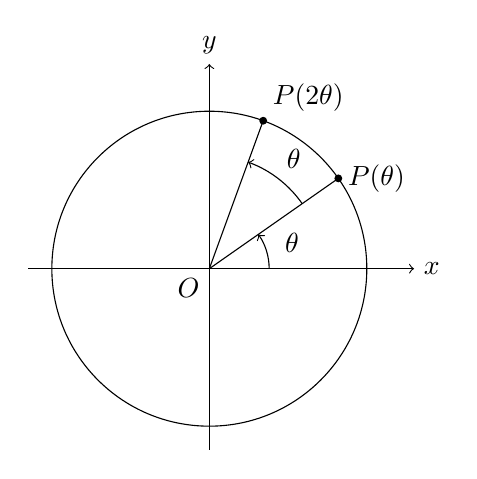
\begin{tikzpicture}[scale=2]
        \draw[->] (-1.15,0) -- (1.3,0) node[right] {$x$};
        \draw[->] (0,-1.15) -- (0,1.3) node[above] {$y$};
        \draw (0,0) circle (1);
        \node[below left] at (0,0) {$O$};
        \draw (0,0) -- (35:1);
        \draw (0,0) -- (70:1);
        \fill (35:1) circle (0.025) node[right] {$P(\theta)$};
        \fill (70:1) circle (0.025) node[above right] {$P(2\theta)$};
        \draw[->] (0.38,0) arc (0:35:0.38);
        \node at (17.5:0.55) {$\theta$};
        \draw[->] (35:0.72) arc (35:70:0.72);
        \node at (52.5:0.88) {$\theta$};
      \end{tikzpicture}
    \end{center}
    
    先ほどの数列では,$a_n$は点$P(\theta_n)$の横座標である.
    回転後の横座標が
    \[
      \cos(2\theta_n)=2\cos^2\theta_n-1=2a_n^2-1
    \]
    となるので,円周上の点の動きを横座標だけで記録したものが,
    漸化式$a_{n+1}=2a_n^2-1$なのである.
    例えば,初めの角度は
    \[
      \frac{\pi}{6}\ \longrightarrow\ \frac{\pi}{3}
      \ \longrightarrow\ \frac{2\pi}{3}
      \ \longrightarrow\ \frac{4\pi}{3}
    \]
    と変わり,横座標は
    \[
      \frac{\sqrt{3}}{2}\ \longrightarrow\ \frac12
      \ \longrightarrow\ -\frac12
      \ \longrightarrow\ -\frac12
    \]
    と変わる.最後の二点は円周上では異なる点だが,横座標は同じである.
    このように,数列の値だけでは見えない点の動きが,角度を使うと見える.
    
    ただし,毎回一定の角$\phi$だけ回す操作では
    $\theta_{n+1}=\theta_n+\phi$となるのに対し,
    ここでは$\theta_{n+1}=2\theta_n$となり,回す角度もそのつど変わる.
    円周上の角度は$2\pi$の整数倍だけ違っても同じ点を表すので,
    点の動きを考えるときは一周ごとに角度を読み替えてよい.
    また,$P(\theta)$と$P(\theta+\pi)$は倍角によって同じ点へ移る.
    したがって,円周全体への写像としての倍角は,一つの一定角の回転とは異なる.
    
    \,\sectionref{節：極形式と複素平面}の見方を使えば,この操作はさらに短く書ける.
    \[
      z_n=\cos\theta_n+i\sin\theta_n
    \]
    と置くと,ド・モアブルの定理より
    \[
      z_{n+1}=z_n^2,\qquad z_n=z_1^{\,2^{n-1}}
    \]
    となる.$|z_n|=1$なので,$z_n$を掛けることは角$\theta_n$の回転である.
    $z_n^2=z_n\cdot z_n$は,現在の点にその点自身を掛けることで,
    角度をもう一度加えている.$a_n$はその実部に当たる.
    
    \subsubsection{正接では直線の傾きを記録する}\label{節：正接では直線の傾きを記録する}
    今度は
    \[
      a_1=\tan\frac{\pi}{12}=2-\sqrt{3},
      \quad
      a_{n+1}=\frac{2a_n}{1-a_n^2}
    \]
    を考える.右辺は$\tan$の倍角公式そのものである.したがって,
    \[
      a_n=\tan\left(2^{n-1}\frac{\pi}{12}\right)
    \]
    と予想できる.
    
    実際,\,$n=1$ で初項に一致し,帰納法の段階では
    \begin{align*}
      a_{n+1}
        &=\frac{2a_n}{1-a_n^2}\\
        &=\cfrac{2\tan\left(2^{n-1}\cfrac{\pi}{12}\right)}
                {1-\tan^2\left(2^{n-1}\cfrac{\pi}{12}\right)}\\
        &=\tan\left(2^n\frac{\pi}{12}\right)
    \end{align*}
    となる.ただし,分母が $0$ になると$\tan$は定義できない.
    三角関数型では,置換を思いつくだけでなく,途中で定義できなくなる項がないかも確認しなければならない.
    
    この場合,$a_n=\tan\theta_n$は,原点と$P(\theta_n)$を通る直線の傾きである.
    直線をさらに$\theta_n$だけ回すと,その傾きが$\tan(2\theta_n)$となる.
    従って,今度は同じ倍角の操作を横座標ではなく傾きとして記録している.
    直線の向きは$\pi$の整数倍だけ違っても同じであり,
    縦向きになると傾きは定義できない.
    $a_n=\pm1$のときは$\cos(2\theta_n)=0$となり,
    この縦向きの状態が漸化式の分母$1-a_n^2=0$に対応する.
    なお,この例の角度は,$n\geq2$では
    \[
      \theta_n=\frac{2^{n-2}\pi}{6}
    \]
    である.$\theta_n=\pi/2+k\pi$となるには$2^{n-2}=3+6k$が必要だが,
    2の累乗は3の倍数ではないので,そのような整数$k$は存在しない.
    初項の角度$\pi/12$でも傾きは定義できるため,この数列はすべての項で定義できる.
    
  \subsubsection{整数倍の公式へ}\label{節：整数倍の公式へ}
    $\cos$の例と$\tan$の例は,同じ方針を共有している.すなわち,
    \[
      a_n=\varphi(\theta_n),
      \quad
      \varphi(m\theta)=F_m(\varphi(\theta))
    \]
    となる関数 $\varphi$ と整数倍公式を探し,角度の漸化式を解いている.
    いわば媒介変数表示や置換のようなことをしている.
    
    また,ここで現れた多項式
    \[
      2x^2-1,
      \quad
      4x^3-3x
    \]
    は偶然の産物ではない.チェビシェフ多項式 $T_m(x)$ を
    \[
      T_m(\cos\theta)=\cos(m\theta)
    \]
    で定義すれば,
    \[
      T_0(x)=1,  T_1(x)=x,
    \]
    \[
      T_{m+1}(x)=2xT_m(x)-T_{m-1}(x)
    \]
    となる.例えば $T_2(x)=2x^2-1$ である.
    したがって,$\cos$の例は
    \[
      a_{n+1}=T_2(a_n),
      \quad
      a_n=T_{2^{n-1}}(a_1)
    \]
    と書き直せる.三角関数の公式から始めて多項式の族へ進む道が,
    付録のチェビシェフ多項式へつながっている.

\subsection{ニュートン法型}\label{節：ニュートン法型}

\noindent\textbf{【前提と学ぶこと】}\par
微分係数$f'(a)$が接線の傾きを表すことを使う.
微分が未習なら,接線と$x$軸の交点から次の近似値を作る図形的な発想と,得られた漸化式の変形を先に読んでよい.
閉じた一般項を求める計算と,近似がどれほど速く改善するかを調べることは別の目標である.
後者は\sectionref*{節：差分から始まる離散的な微積分}で見直す.

少々離れたところから話を始める.
ある関数$f(x)$について,\,$f(a)$が既知の時,その近傍の点$x=a+h$で
\[
  f(a+h) \approx f(a)+f'(a)h
\]
が成り立つ.
つまり,\,$f(a)$の値を元に,\,$f(a+h)$を近似したのである.
方程式
\[
  f(x)=x^2-2=0
\]
の正の解 $\sqrt{2}$ を求めたいとする.いまの近似値を $x=a_n$ とし,
点 $(a_n,f(a_n))$ における接線を引く.その接線の傾きは
$f'(a_n)=2a_n$ だから,接線の方程式は
\[
  y=f(a_n)+2a_n(x-a_n)
\]
である.\,$y=0$ と置いて $x$ 軸との交点を求めると,
\begin{align*}
  a_{n+1}
    &=a_n-\frac{f(a_n)}{f'(a_n)}\\
    &=a_n-\frac{a_n^2-2}{2a_n}\\
    &=\frac{a_n^2+2}{2a_n}
\end{align*}
これが
\[
  a_{n+1}=\frac{a_n^2+2}{2a_n}
\]
という,ニュートン法を$f(x)=x^2-2$に適用したときの漸化式である.

例えば $a_1=2$ とすると,
\[
  a_2=\frac{3}{2},
  \quad
  a_3=\frac{17}{12},
  \quad
  a_4=\frac{577}{408}
\]
となり,これらは $\sqrt{2}$ に急速に近づく.この速さは,誤差を
$e_n=a_n-\sqrt{2}$ と置くと見える.
\begin{align*}
  e_{n+1}
    &=\frac{a_n^2+2}{2a_n}-\sqrt{2}\\
    &=\frac{(a_n-\sqrt{2})^2}{2a_n}\\
    &=\frac{e_n^2}{2a_n}
\end{align*}
誤差がほぼ二乗されるため,正しい近似に近づくと桁数が一気に増える.

実は,この漸化式は閉じた式で表すことができる.
\[
  a_{n+1}-\sqrt{2}=\frac{(a_n-\sqrt{2})^2}{2a_n},
  \qquad
  a_{n+1}+\sqrt{2}=\frac{(a_n+\sqrt{2})^2}{2a_n}
\]
であることに注目すると,両辺の比を取ることで$2a_n$が消え,
\[
  \frac{a_{n+1}-\sqrt{2}}{a_{n+1}+\sqrt{2}}
  =\left(\frac{a_n-\sqrt{2}}{a_n+\sqrt{2}}\right)^{2}
\]
という関係が得られる.つまり
\[
  b_n=\frac{a_n-\sqrt{2}}{a_n+\sqrt{2}}
\]
と置くと,\,$b_{n+1}=b_n^{2}$という,対数型(\sectionref{節：対数型})と同じ構造の漸化式になる.先ほど見た誤差の2乗のふるまいは,この$b_{n+1}=b_n^2$そのものだったのである.

\,$a_1=2$のとき,\,$b_1=\dfrac{2-\sqrt2}{2+\sqrt2}=3-2\sqrt2=\dfrac1{3+2\sqrt2}$であるから,\,$u=3+2\sqrt2$とおくと$b_n=u^{-2^{n-1}}$である.これを$b_n=\dfrac{a_n-\sqrt2}{a_n+\sqrt2}$について$a_n$で解けば,
\[
  a_n=\sqrt{2}\,\frac{u^{2^{n-1}}+1}{u^{2^{n-1}}-1},\qquad u=3+2\sqrt2
\]
という閉じた式が得られる.

このように,今回の$f(x)=x^2-2$に対するニュートン法型漸化式では,特別な変形によって一般項を閉じた式で表すことができる.
しかし,一般のニュートン法型漸化式が同じように閉じた式で表せるとは限らない.
閉じた式が得られなくても,収束先や誤差の減り方を調べることには十分な価値がある.
この解法の主眼は閉じた式を得ることだけにあるのではない.
「接線を使って,次の近似値をどう設計するか」を考え,その設計が
どのような速さで誤差を減らすかを調べることこそが本質である.付録では,この考えを
漸化式の収束,固定点,誤差評価,微分方程式の数値解法へ広げる.

\subsection{初項依存型}\label{節：初項依存型}
  \BookFigCobweb

  図では$f(x)=\displaystyle\frac{x^2-1}{2}$として,
  横軸上の$a_1=2$から曲線$y=f(x)$へ縦に進み,
  直線$y=x$へ横に進む操作を繰り返している.
  縦の移動は$a_{n+1}=f(a_n)$という計算そのものであり,
  横の移動で得られた値を次の入力として読む.
  最初の三つの入力は$a_1=2,\,a_2=\displaystyle\frac32,\,
  a_3=\displaystyle\frac58$に対応する.
  初項を変えれば出発点が変わり,同じ更新規則でも別の軌道になる.



最後に,\bookterm{recurrence}{漸化式}の形だけでなく,初項の選び方そのものが問題を左右する
例を見よう.
\[
  a_1=c,
  \quad
  a_{n+1}=\frac{a_n^2-1}{2}
\]
初項を記号 $c$ のままにすると,
\begin{align*}
  a_2&=\frac{c^2-1}{2},\\
  a_3&=\frac{c^4-2c^2-3}{8},\\
  a_4&=\frac{c^8-4c^6-2c^4+12c^2-55}{128}
\end{align*}
一般に $a_n$ は $c$ の次数 $2^{n-1}$ の多項式になる.初項を一般の
文字のまま扱おうとすると,項を一つ進めるたびに次数が倍になり,
\bookterm{trigonometric}{三角関数}型や基本対称式型のような固定された表現が見えてこない.

特に $c=2$ と固定すると,
\[
  a_1=2,
  \quad
  a_2=\frac{3}{2},
  \quad
  a_3=\frac{5}{8},
  \quad
  a_4=-\frac{39}{128}
\]
となる.しかし,この列は直前の例のように角度を2倍する形にも,
指数の差を保つ形にも,接線近似の形にもならない.

このように$c=2$では,ここまでに試した変換から直ちに簡単な表現を見出せない.ただし,数項の計算だけで,他の初項についても簡単な表現が存在しないとは結論できない.
一方で,初項をうまく選べば特別な構造が現れることもある.
例えば定\bookterm{sequence}{数列}を探すだけなら,
\[
  c=1+\sqrt{2},
  \quad
  c=1-\sqrt{2}
\]
では $a_{n+1}=a_n=c$ となる.大切なのは,ある初項を選んだときだけ
特別な恒等式や置換が働くことがあり,初項を一般化するとその偶然の
構造が失われる,という事実である.

初項によって解法の見通しが変わる例は,先に挙げた基本対称式型にもある.
もちろん,一般の初項での解法は先に示したとおりであるが,より狭義の解き方ではこのようなものがある.
\[
  a_1=-1,\quad a_{n+1}=a_n^2-2
\]
のような場合であれば,第5項までが以下のようになる.
\[
  -1,-1,-1,-1,-1
\]
\bookterm{recurrence}{漸化式}が表す\bookterm{sequence}{数列}が定数\bookterm{sequence}{数列}を成したのだ.
このような解はシンプルに\bookterm{fixed}{不動点}を求めることで作り出せる.
つまりは
\[
  \alpha=\alpha^2-2
\]
を$\alpha$について解けばよい.
この二次方程式の解は$\alpha=-1,2$である.
\,$\alpha=2$を初項に選ぶと,\bookterm{recurrence}{漸化式}から常に$a_n=2$となる.

実は,この定\bookterm{sequence}{数列}$a_n=-1$は,\,\sectionref{節：基本対称式型}で扱った$a_{n+1}=a_n^2-2$型の特別な場合と見ることができる.
\,$\alpha+\alpha^{-1}=a_1$を満たす$\alpha$が単位円上,すなわち$\alpha=e^{i\theta}$となるように($-2\le a_1\le2$のように)初項を選べば,
\[
  a_n=\alpha^{2^{n-1}}+\alpha^{-2^{n-1}}=2\cos(2^{n-1}\theta)
\]
という\bookterm{trigonometric}{三角関数}の形になる.今回の$a_1=-1$はまさにこの場合で,\,$2\cos\theta=-1$すなわち$\theta=\dfrac{2\pi}3$ととれる.このとき$2^{n-1}\theta$は$2$倍するごとに$\dfrac{2\pi}3$と$\dfrac{4\pi}3$を行き来し(どちらも余弦は$-\dfrac12$),\,$a_n=2\cos(2^{n-1}\theta)=-1$が常に成り立つ.つまり$a_1=-1$は,角度を$2$倍しても余弦の値が変わらないという特別な初項を選んだ場合に他ならない.

この例では,少なくとも本節で扱った初等的な道具からは\bookterm{general}{一般項}を得る
決まった方法が出てこない.それでも\bookterm{recurrence}{漸化式}は\bookterm{sequence}{数列}を定めており,
\[
  a_n=f^{\,\circ(n-1)}(c),
  \quad
  f(x)=\frac{x^2-1}{2}
\]
と書くことはできる.これは解答の終わりではなく,「\bookterm{general}{一般項}を求める」
という目標自体を見直す入口である.付録では,閉じた式が得られない
場合にも,軌道,\bookterm{limit}{極限},近似,\bookterm{matrix}{行列},\bookterm{generating}{母関数}など別の言葉で\bookterm{sequence}{数列}を理解する
方法を考える.


\end{bookcolumns}
